\clearpage
\bookpart{概率的测度基础}{Measure-Theoretic Probability}
\label{part:measure-theoretic-probability}

\BookPartGuide{%
第一部分把概率写成计数或密度的积分。可是有些随机结果既没有概率表，也没有普通的密度；给定一个观测值之后再求平均，也会遇到“条件事件的概率为零”的困难。这些问题需要用测度把概率模型统一起来。

第~\ref{chap:probability-spaces}章回用卷四的测度与积分，建立概率空间、随机变量与分布，把期望统一成积分。第~\ref{chap:conditional-expectation}章研究给定信息之后怎样求平均：从有限分组的组内平均出发，定义条件期望，建立它的运算规则，并说明它是均方意义下最好的预测。第~\ref{chap:conditional-distributions}章进一步研究给定观测后的完整概率规律，建立条件分布、联合分布的分解与条件独立。

随时间展开的信息流、鞅和转移过程属于随机过程，在卷九研究。}

\chapter{概率空间}
\label{chap:probability-spaces}

在长为$1$的木棍上随机取一点，它落在有理数上的概率是多少？顾客来到窗口，有三成机会不用等，否则等待时间按指数规律分布，平均要等多久？反复抛一枚公平硬币，把正反面写成三进制小数得到的Cantor变量，平均值又是多少？这些问题在第一部分都出现过，却都没有得到完整的回答。概率表只能处理有限或可数个取值，密度只能处理“单位长度上有质量”的情形，等待时间两者都不是，Cantor变量更是两者都用不上。

困难不在计算技巧，而在模型本身没有说清楚。哪些集合可以问概率？概率对无穷多个事件怎样相加？“随机变量”这个函数要满足什么条件，才能保证“它落在某个范围内”是一个有概率的事件？期望既然有时是和、有时是积分，它们背后是不是同一个运算？卷四的测度与积分正好回答了这些问题，本章把它们翻译成概率的语言。

路线如下。先确定可以问概率的事件族，再把概率规定为总质量为一的测度，由可数可加性得到概率的连续性，并说明零概率事件和完备化各自起什么作用。然后把随机变量推广为可测映射，用它生成的事件族表达一次观测提供的信息；把分布定义为取值空间上的推前测度，区分处处相等、几乎必然相等和同分布。接着用乘积测度构造独立的随机对象，包括独立序列。最后把期望统一为概率测度上的积分，第一部分的求和公式、密度积分以及独立乘积的计算都成为它的特例。

全章反复使用四个模型：两枚骰子的$36$个等可能结果；木棍上的均匀随机点，样本空间是$[0,1)$，概率是长度；有三成机会不用等的等待时间$W$；以及Cantor变量。读者需要熟悉第一部分的概率表、密度和分布函数，以及卷四的$\sigma$代数、测度、可测映射和积分。

\section{事件与可测结构}
\label{sec:pspace-events}

在有限的古典模型里，样本空间的每个子集都是事件，都可以问概率。木棍上的随机点也能这样处理吗？回答这个问题之前，先看三种情形，它们分别从不同方向说明：事件族需要单独指定，不能默认是样本空间的全部子集。

\paragraph{连续位置}
木棍上的随机点取值于$\Omega=[0,1)$，我们要求区间的概率等于它的长度。由此出发，区间的有限并、补集都有自然的概率；有理数集$\mathbb{Q}\cap[0,1)$是可数个单点之并，也应当有概率。可是能不能给$[0,1)$的\emph{每个}子集都指定一个“长度”，同时保持区间长度不变、平移不变和可数可加？卷四给出了否定的回答：用选择公理构造的Vitali集在这些要求下无法赋值，可参考\BookChapterRef{chap:measure}{卷四第5章“测度”}。所以对连续位置，我们只能对一部分子集谈概率。

\paragraph{混合的取值}
等待时间$W$以概率$0.3$恰好取$0$，其余$0.7$的质量按密度$0.7\,\mathrm{e}^{-t}$铺在$(0,\infty)$上。要描述它，单点$\{0\}$必须是事件，各种区间也必须是事件，而且两种事件要能一起运算，例如“$W$等于$0$或大于$2$”。概率表只处理可数个点，密度只处理区间上的积分，事件族必须同时容纳两者。

\paragraph{不同的记录方式}
掷两枚骰子，样本空间是$36$个有序对$(i,j)$。如果观察者只被告知点数和$S=i+j$，他能判断哪些事件是否发生？“$S=7$”可以，“$S$是偶数”也可以，但“第一枚是$1$”不行：$S=7$时第一枚可能是$1$，也可能是$6$。图~\ref{fig:pspace-dice-partitions}(a)中红框是事件“第一枚是$1$”，它横跨了点数和不同的六个格子，只取其中各一个格子。在同一个样本空间上，可以判断的事件族取决于观察到了什么。

\begin{BookInlineFigure}
  \centering
  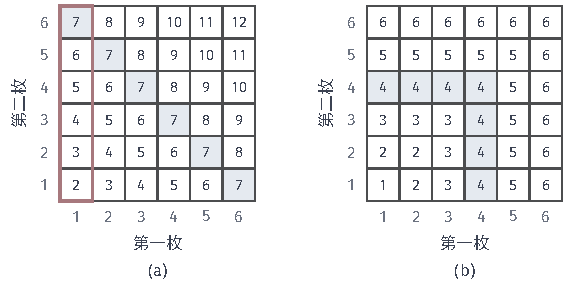
\includegraphics[width=96mm]{figures/07-probability/02-measure-theoretic-probability/tikz/pspace-dice-partitions/figure.pdf}
  \caption{同一个样本空间上的两种记录。每个格子是一个有序结果$(i,j)$。(a)格内是点数和$S$，浅蓝格子组成$\{S=7\}$；红框是事件“第一枚是$1$”，它把$S$取值相同的格子拆开了，只知道$S$无法判断它是否发生。(b)格内是较大点数$M$，浅蓝的L形区域是$\{M=4\}$。}
  \label{fig:pspace-dice-partitions}
\end{BookInlineFigure}

三种情形的共同点是：样本空间$\Omega$回答“可能出现哪些结果”，另需一个子集族回答“可以对哪些结果集合问概率”。前者是试验的描述，后者是我们愿意且能够提问的范围。

\paragraph{事件族应满足的运算}
什么样的子集族适合做事件族？从提问的角度看，至少有三条要求。整个$\Omega$应当是事件，“某个结果出现了”总能回答。若能判断$A$是否发生，也就能判断$A$不发生，所以事件族对补集封闭。若能逐一判断$A_1,A_2,\dots$是否发生，就应当能判断“其中至少一个发生”，所以事件族对可数并封闭。

为什么要求可数并而不只是有限并？第~\ref{chap:classical-probability}章抛硬币直到出现正面，事件“迟早出现正面”是“第$k$次首次出现正面”对$k=1,2,\dots$之并；有理数集是可数个单点之并。概率论中的极限陈述，例如“平均值收敛”，也都要用可数次并与交写出来。只要求有限并的事件族装不下这些事件。

这三条恰好是卷四$\sigma$代数的定义。设$\mathcal{F}$是$\Omega$的子集族，满足：
\begin{enumerate}
  \item $\Omega\in\mathcal{F}$；
  \item 若$A\in\mathcal{F}$，则$A^{\mathrm{c}}\in\mathcal{F}$；
  \item 若$A_1,A_2,\dots\in\mathcal{F}$，则$\bigcup_{k}A_k\in\mathcal{F}$。
\end{enumerate}
称$\mathcal{F}$为$\Omega$上的$\sigma$代数，$(\Omega,\mathcal{F})$为可测空间。由补集和可数并还能得到可数交：
\[
  \bigcap_{k}A_k=\Bigl(\bigcup_{k}A_k^{\mathrm{c}}\Bigr)^{\mathrm{c}}\in\mathcal{F},
\]
以及$\varnothing=\Omega^{\mathrm{c}}\in\mathcal{F}$、差集$A\setminus B=A\cap B^{\mathrm{c}}\in\mathcal{F}$。

\begin{definition}[事件]
\label{def:pspace-event}
设$(\Omega,\mathcal{F})$是可测空间。$\mathcal{F}$中的集合称为事件，$\mathcal{F}$称为\term{事件族}（family of events）。
\end{definition}

从此“事件”是一个相对于$\mathcal{F}$的概念。$\Omega$的子集未必是事件；同一个$\Omega$配上不同的$\mathcal{F}$，描述的是同一组结果上不同的提问范围。第一部分在有限或可数的$\Omega$上取全部子集，在实轴上只对区间及其有限并谈概率，都是这里的特例或其中的一部分。

\paragraph{有限样本空间上的事件族}
$\Omega$有限时，$\sigma$代数有一个具体的样子：它把$\Omega$分成若干块，事件恰好是若干块的并。块的构造是取包含某个点的所有事件之交。对$\omega\in\Omega$，令
\begin{equation}
  A(\omega)=\bigcap\{A\in\mathcal{F}:\omega\in A\},
  \label{eq:pspace-atom}
\end{equation}
称为$\omega$所在的\term{原子}（atom）。$\mathcal{F}$是有限族，所以这是有限交，$A(\omega)\in\mathcal{F}$。它是包含$\omega$的最小事件。

\begin{lemma}[有限样本空间上的$\sigma$代数]
\label{lem:pspace-finite-atoms}
设$\Omega$有限，$\mathcal{F}$是$\Omega$上的$\sigma$代数。则不同的原子两两不交，它们构成$\Omega$的一个划分；$\mathcal{F}$中每个事件都是若干个原子之并。若原子共有$k$个，则$\mathcal{F}$恰有$2^{k}$个事件。
\end{lemma}

\begin{proof}
先证两个原子要么相同、要么不交。设$A(\omega)\cap A(\omega')\neq\varnothing$。若$\omega\notin A(\omega')$，则$A(\omega)\setminus A(\omega')$是包含$\omega$的事件，且比$A(\omega)$小，与$A(\omega)$的最小性矛盾。所以$\omega\in A(\omega')$，于是$A(\omega)\subseteq A(\omega')$。对称地$A(\omega')\subseteq A(\omega)$，两者相同。

再证每个事件是原子之并。设$A\in\mathcal{F}$。对每个$\omega\in A$，$A$是包含$\omega$的事件，所以$A(\omega)\subseteq A$。于是
\[
  A=\bigcup_{\omega\in A}A(\omega),
\]
右边是若干个原子之并。反过来，原子都是事件，有限个事件之并仍是事件。所以$\mathcal{F}$恰由原子的各种并组成。$k$个两两不交的原子，每个选或不选，给出$2^{k}$个不同的并。
\end{proof}

在骰子的例子里，只知道$S$的观察者能判断的事件族，以$S$的$11$个取值对应的格子组为原子，即图~\ref{fig:pspace-dice-partitions}(a)中的各条反对角线。由引理~\ref{lem:pspace-finite-atoms}，这个事件族有$2^{11}=2048$个事件，而$36$个结果的全部子集有$2^{36}$个。“第一枚是$1$”不是原子之并，所以不在其中。只知道较大点数$M$的观察者，原子是图~\ref{fig:pspace-dice-partitions}(b)中的$6$个L形区域，事件族有$2^{6}=64$个事件。

\paragraph{生成的事件族}
实际建模时，我们通常只知道几个“想问的事件”，并不想逐一列出整个$\sigma$代数。卷四给出了办法：对$\Omega$的任意子集族$\mathcal{C}$，包含$\mathcal{C}$的所有$\sigma$代数之交仍是$\sigma$代数，它是包含$\mathcal{C}$的最小$\sigma$代数，记作$\sigma(\mathcal{C})$。它就是从$\mathcal{C}$出发、反复做补集与可数并所能得到的全部事件。

最简单的情形是一个事件$A$。包含$A$的$\sigma$代数必须含有$\Omega$、$A$和$A^{\mathrm{c}}$，因而含有$\varnothing$，而这四个集合已经对补集和并封闭，所以
\[
  \sigma(\{A\})=\{\varnothing,A,A^{\mathrm{c}},\Omega\}.
\]
两个相交的事件$A,B$把$\Omega$切成四块（图~\ref{fig:pspace-generated-events}）。四块都要在$\sigma(\{A,B\})$中，而它们的各种并已经构成$\sigma$代数，所以$\sigma(\{A,B\})$恰有$2^{4}=16$个事件。

\begin{BookInlineFigure}
  \centering
  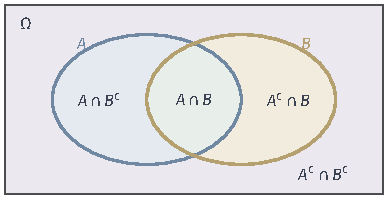
\includegraphics[width=66mm]{figures/07-probability/02-measure-theoretic-probability/tikz/pspace-generated-events/figure.pdf}
  \caption{两个事件$A$（蓝框）与$B$（黄框）把$\Omega$切成四个原子：$A\cap B^{\mathrm{c}}$（浅蓝）、$A\cap B$（浅绿）、$A^{\mathrm{c}}\cap B$（浅黄）和$A^{\mathrm{c}}\cap B^{\mathrm{c}}$（浅紫）。$\sigma(\{A,B\})$由这四块的全部$16$种并组成。}
  \label{fig:pspace-generated-events}
\end{BookInlineFigure}

对木棍上的随机点，想问的事件是区间。由区间生成的$\sigma$代数就是卷四的Borel $\sigma$代数，记作$\mathcal{B}([0,1))$。它不仅含有区间，还含有单点$\{x\}=\bigcap_n[x,x+1/n)$、有理数集、无理数集以及Cantor集等用可数次运算得到的集合。我们无法把它的成员一一列出，但对每个具体的集合，只要说出它怎样由区间经可数次运算得到，就知道它是事件。实轴上的$\mathcal{B}(\mathbb{R})$、$d$维空间上的$\mathcal{B}(\mathbb{R}^{d})$同理，它们也可以分别由半直线$(-\infty,x]$、左下象限$(-\infty,x_1]\times\cdots\times(-\infty,x_d]$生成。

表~\ref{tab:pspace-event-families}汇总了本章常用模型的样本空间与事件族。

\begin{BookInlineTable}
  \centering
  \caption{常用模型的样本空间与事件族}
  \label{tab:pspace-event-families}
  \begin{tabular}{lll}
    \toprule
    模型 & 样本空间$\Omega$ & 事件族$\mathcal{F}$ \\
    \midrule
    两枚骰子 & $36$个有序对 & 全部子集 \\
    只知道点数和 & $36$个有序对 & $\sigma(S)$，$2^{11}$个事件 \\
    木棍上的点 & $[0,1)$ & $\mathcal{B}([0,1))$ \\
    等待时间$W$ & $\mathbb{R}$ & $\mathcal{B}(\mathbb{R})$ \\
    \bottomrule
  \end{tabular}
\end{BookInlineTable}

表中的$\sigma(S)$是由点数和生成的事件族，第~\ref{sec:pspace-random-objects}节对一般的观测给出它的定义。

\section{概率测度}
\label{sec:pspace-measures}

事件族确定以后，要给每个事件指定一个概率。第~\ref{chap:classical-probability}章已经列出了三条要求：概率非负，必然事件的概率为$1$，互斥事件的概率相加。那一章的末尾还看到，抛硬币直到出现正面时，可加性必须对可数多个互斥事件成立，各次首次出现正面的概率$2^{-k}$加起来才等于$1$。把这些要求放在一起，概率就是卷四中总质量为一的测度。

\begin{definition}[概率测度与概率空间]
\label{def:pspace-probability-space}
设$(\Omega,\mathcal{F})$是可测空间。函数$\mathbb{P}:\mathcal{F}\to[0,1]$若满足$\mathbb{P}(\Omega)=1$，并且对任意两两不交的事件$A_1,A_2,\dots$有
\begin{equation}
  \mathbb{P}\Bigl(\bigcup_{k=1}^{\infty}A_k\Bigr)=\sum_{k=1}^{\infty}\mathbb{P}(A_k),
  \label{eq:pspace-countable-additivity}
\end{equation}
则称$\mathbb{P}$为\term{概率测度}（probability measure），称$(\Omega,\mathcal{F},\mathbb{P})$为\term{概率空间}（probability space）。
\end{definition}

式~\eqref{eq:pspace-countable-additivity}称为可数可加性。取$A_k=\varnothing$（$k>n$）就得到有限可加性，所以第一部分使用的规则都保留下来：补事件的概率$\mathbb{P}(A^{\mathrm{c}})=1-\mathbb{P}(A)$；单调性，即$A\subseteq B$时$\mathbb{P}(A)\leq\mathbb{P}(B)$；以及联合界
\[
  \mathbb{P}\Bigl(\bigcup_kA_k\Bigr)\leq\sum_k\mathbb{P}(A_k),
\]
它对可数个事件也成立。这些都是卷四测度基本性质的特例。

把概率看成单位质量的分配，可数可加性说的是：把一块区域切成可数多块，各块质量之和等于整块的质量。它不允许质量在“切成无穷多块”的过程中凭空出现或消失。下面先看这条要求带来的第一个后果。

\paragraph{概率的连续性}
事件常常由一列事件逼近：$\{W\leq1/n\}$随$n$增大而缩小，极限是$\{W\leq0\}$；“前$n$次中出现过正面”随$n$增大而扩大，极限是“迟早出现正面”。概率是否随事件一起取极限？

\begin{theorem}[概率的连续性]
\label{thm:pspace-continuity}
设$(\Omega,\mathcal{F},\mathbb{P})$是概率空间。
\begin{enumerate}
  \item 若$A_1\subseteq A_2\subseteq\cdots$，令$A=\bigcup_nA_n$，则
  \begin{equation}
    \mathbb{P}(A)=\lim_{n\to\infty}\mathbb{P}(A_n);
    \label{eq:pspace-continuity-up}
  \end{equation}
  \item 若$B_1\supseteq B_2\supseteq\cdots$，令$B=\bigcap_nB_n$，则
  \begin{equation}
    \mathbb{P}(B)=\lim_{n\to\infty}\mathbb{P}(B_n).
    \label{eq:pspace-continuity-down}
  \end{equation}
\end{enumerate}
\end{theorem}

\begin{proof}
先证递增的情形。把$A$切成互不相交的“新增部分”：令$C_1=A_1$，$C_k=A_k\setminus A_{k-1}$（$k\geq2$）。各$C_k$两两不交，且
\[
  A_n=\bigcup_{k=1}^{n}C_k,\qquad A=\bigcup_{k=1}^{\infty}C_k .
\]
由可数可加性与有限可加性，
\[
  \mathbb{P}(A)=\sum_{k=1}^{\infty}\mathbb{P}(C_k)=\lim_{n\to\infty}\sum_{k=1}^{n}\mathbb{P}(C_k)=\lim_{n\to\infty}\mathbb{P}(A_n).
\]

递减的情形取补集。$B_n^{\mathrm{c}}$递增，并集是$B^{\mathrm{c}}$，由第一部分，
\[
  1-\mathbb{P}(B)=\mathbb{P}(B^{\mathrm{c}})=\lim_{n\to\infty}\mathbb{P}(B_n^{\mathrm{c}})=1-\lim_{n\to\infty}\mathbb{P}(B_n).
\]
两边消去$1$即得式~\eqref{eq:pspace-continuity-down}。
\end{proof}

证明中递减情形用到了$\mathbb{P}(\Omega)=1$有限。对一般的测度，递减情形需要$B_1$的测度有限，例如实轴上的$[n,\infty)$递减到空集，长度却一直是无穷。概率测度总质量为一，这个条件自动满足。反过来，若一个集函数有限可加，又满足式~\eqref{eq:pspace-continuity-up}，取$A_n=C_1\cup\cdots\cup C_n$即可推出可数可加性。所以对有限可加的概率，“可数可加”与“沿递增序列连续”是同一个要求。

\paragraph{分布函数的性质}
连续性的第一个用途是补上第~\ref{chap:random-variables}章留下的证明：分布函数的基本性质对一般分布都成立。那里的分布是实轴上的概率，这里设$P$是$(\mathbb{R},\mathcal{B}(\mathbb{R}))$上的任一概率测度，令
\begin{equation}
  F(x)=P\bigl((-\infty,x]\bigr),\qquad x\in\mathbb{R}.
  \label{eq:pspace-cdf}
\end{equation}

$F$单调不减，因为$x<y$时$(-\infty,x]\subseteq(-\infty,y]$。对右连续性，取$x_n\downarrow x$，则$(-\infty,x_n]$递减，交集为$(-\infty,x]$，由式~\eqref{eq:pspace-continuity-down}得$F(x_n)\to F(x)$。同理，$(-\infty,-n]$递减到空集，$(-\infty,n]$递增到$\mathbb{R}$，所以
\[
  \lim_{x\to-\infty}F(x)=0,\qquad \lim_{x\to+\infty}F(x)=1 .
\]

左极限也有明确含义。取$x_n\uparrow x$且$x_n<x$，区间$(-\infty,x_n]$递增，并集是$(-\infty,x)$，于是
\[
  F(x^{-})=\lim_{n\to\infty}F(x_n)=P\bigl((-\infty,x)\bigr),
\]
跳跃高度$F(x)-F(x^{-})=P(\{x\})$正是单点的概率。这几步在第一部分只对概率表和密度验证过，现在对任何概率测度都成立，因为它们只用到可数可加性。

用等待时间$W$看一看这两个方向的极限。$W$的分布是
\begin{equation}
  P_W(A)=0.3\cdot\mathbf{1}_{A}(0)+0.7\int_{A\cap(0,\infty)}\mathrm{e}^{-t}\,\mathrm{d}t,\qquad A\in\mathcal{B}(\mathbb{R}),
  \label{eq:pspace-waiting-law}
\end{equation}
它的分布函数在$t\geq0$时为$F_W(t)=0.3+0.7(1-\mathrm{e}^{-t})$。从右侧逼近$0$，四个值是
\[
  F_W(1)\approx0.7425,\quad F_W(\tfrac12)\approx0.5754,\quad F_W(\tfrac14)\approx0.4548,\quad F_W(\tfrac18)\approx0.3823,
\]
它们递减到$F_W(0)=0.3$。从左侧逼近，$F_W(-1/n)=0$，极限是$P_W((-\infty,0))=0$。两侧极限之差$0.3$就是$P_W(\{0\})$，见图~\ref{fig:pspace-continuity}。

\begin{BookInlineFigure}
  \centering
  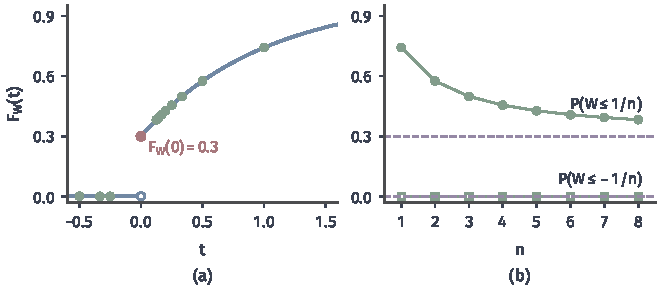
\includegraphics[width=112mm]{figures/07-probability/02-measure-theoretic-probability/matplotlib/pspace-continuity/figure.pdf}
  \caption{等待时间$W$的分布函数与概率的连续性。(a)蓝线是$F_W$，空心点是$0$处的左极限，红点是$F_W(0)=0.3$；右侧绿点是$t=1/n$处的值，左侧绿点是$t=-1/n$处的值。(b)绿色实心点是递减事件$\{W\leq1/n\}$的概率，趋于$0.3$；空心方块是递增事件$\{W\leq-1/n\}$的概率，恒为$0$。紫色虚线是两个极限。}
  \label{fig:pspace-continuity}
\end{BookInlineFigure}

\paragraph{已有模型怎样成为概率空间}
第一部分的每个模型都可以写成一个概率空间，只是事件族和概率的给法不同。

古典模型取$\Omega$有限，$\mathcal{F}$为全部子集，$\mathbb{P}(A)=\lvert A\rvert/\lvert\Omega\rvert$。有限个集合不可能有无穷多个两两不交的非空成员，可数可加性归结为有限可加性，也就是计数的加法。

概率表取$\Omega$可数，$\mathcal{F}$为全部子集，给每个$\omega$一个$p(\omega)\geq0$，且$\sum_{\omega}p(\omega)=1$，令$\mathbb{P}(A)=\sum_{\omega\in A}p(\omega)$。对两两不交的$A_1,A_2,\dots$，
\[
  \mathbb{P}\Bigl(\bigcup_{k}A_k\Bigr)=\sum_{k}\sum_{\omega\in A_k}p(\omega)=\sum_{k}\mathbb{P}(A_k),
\]
第一个等号把并集中的点按所属的$A_k$分组。非负项级数可以任意重排、分组而和不变，这就是可数可加性。

密度模型取$\Omega=\mathbb{R}$，$\mathcal{F}=\mathcal{B}(\mathbb{R})$。给定非负Borel函数$f$且$\int_{\mathbb{R}}f\,\mathrm{d}\lambda=1$，其中$\lambda$是Lebesgue测度，令
\begin{equation}
  \mathbb{P}(A)=\int_{A}f\,\mathrm{d}\lambda,\qquad A\in\mathcal{B}(\mathbb{R}).
  \label{eq:pspace-density-model}
\end{equation}
对两两不交的$A_k$，被积函数可以逐项拆开：
\[
  \mathbf{1}_{\bigcup_kA_k}f=\sum_k\mathbf{1}_{A_k}f,
\]
右边的部分和是递增的非负函数列。由单调收敛定理，积分与求和可以交换，于是式~\eqref{eq:pspace-density-model}可数可加。在区间上，这个积分与第一部分的黎曼积分（含反常积分）一致，可参考\BookChapterRef{chap:integration}{卷四第6章“积分”}。

混合模型把两者相加。式~\eqref{eq:pspace-waiting-law}中，$A\mapsto\mathbf{1}_{A}(0)$是$0$处的单点测度，第二项是密度为$\mathrm{e}^{-t}\mathbf{1}_{\{t>0\}}$的测度。非负系数的测度之和仍是测度，总质量$0.3+0.7=1$，所以$P_W$是概率测度。单点$\{0\}$和各种区间在同一个$\mathcal{B}(\mathbb{R})$中，可以一起运算。

\paragraph{由分布函数给出的模型}
Cantor分布既没有概率表也没有密度，它只有分布函数。第~\ref{chap:random-variables}章说过，满足三条性质的函数都可以用来规定模型；现在可以说清这句话的含义。

\begin{theorem}[分布函数确定实轴上的概率]
\label{thm:pspace-cdf-measure}
设$F:\mathbb{R}\to[0,1]$单调不减、右连续，且$\lim_{x\to-\infty}F(x)=0$，$\lim_{x\to+\infty}F(x)=1$。则$(\mathbb{R},\mathcal{B}(\mathbb{R}))$上存在唯一的概率测度$P$，使得
\begin{equation}
  P\bigl((-\infty,x]\bigr)=F(x),\qquad x\in\mathbb{R}.
  \label{eq:pspace-cdf-measure}
\end{equation}
\end{theorem}

\begin{proof}
存在性就是卷四的Stieltjes测度定理：对单调不减、右连续的$F$，存在$\mathcal{B}(\mathbb{R})$上的测度$P$，使$P((a,b])=F(b)-F(a)$对一切$a<b$成立。令$a\to-\infty$，由连续性得
\[
  P\bigl((-\infty,b]\bigr)=\lim_{a\to-\infty}\bigl(F(b)-F(a)\bigr)=F(b).
\]
再令$b\to+\infty$得$P(\mathbb{R})=1$。

唯一性用卷四的$\pi$--$\lambda$定理。半直线族$\{(-\infty,x]:x\in\mathbb{R}\}$对有限交封闭，因为$(-\infty,x]\cap(-\infty,y]=(-\infty,\min\{x,y\}]$，所以它是$\pi$系统，并且生成$\mathcal{B}(\mathbb{R})$。两个概率测度若在一个生成$\sigma$代数的$\pi$系统上一致，就在整个$\sigma$代数上一致。满足式~\eqref{eq:pspace-cdf-measure}的两个概率测度在半直线上一致，因此相同。
\end{proof}

这个定理有两层意思。唯一性说，分布函数记录了实轴上全部Borel集的概率，而不只是区间的概率；第一部分只能从$F$读出区间的概率，现在知道其余集合的概率也已被确定。存在性说，Cantor函数确实对应一个概率测度，第~\ref{chap:random-variables}章的Cantor分布不是一个只有分布函数的“形式对象”。

\paragraph{单点的概率与总概率}
木棍上的均匀随机点由$\Omega=[0,1)$、$\mathcal{F}=\mathcal{B}([0,1))$和长度测度$\lambda$给出。每个单点的概率为零：对任意$h>0$，$\{x\}\subseteq[x,x+h)$，所以$\lambda(\{x\})\leq h$，再令$h\to0$。由可数可加性，任何可数集的概率也为零，特别地
\[
  \mathbb{P}\bigl(\mathbb{Q}\cap[0,1)\bigr)=\sum_{q}\lambda(\{q\})=0 .
\]

不借助单点的结论，也可以直接看到有理数集“太稀”。把有理数排成一列$q_1,q_2,\dots$，用以$q_k$为中心、长$\varepsilon/2^{k}$的区间覆盖它，总长度不超过$\varepsilon$（图~\ref{fig:pspace-rational-cover}）。$\varepsilon$可以任意小，所以有理数集的概率为零，尽管有理数在$[0,1)$中处处稠密。

\begin{BookInlineFigure}
  \centering
  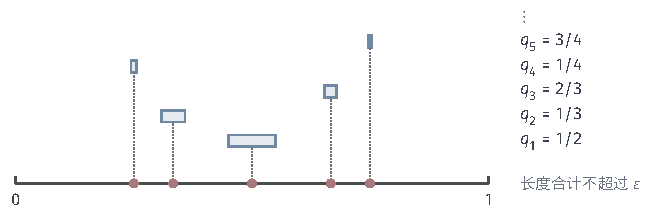
\includegraphics[width=104mm]{figures/07-probability/02-measure-theoretic-probability/tikz/pspace-rational-cover/figure.pdf}
  \caption{用总长度不超过$\varepsilon$的区间覆盖$[0,1)$中的有理数，这里$\varepsilon=0.2$。红点是按某种次序排列的前五个有理数$q_k$，浅蓝区间以$q_k$为中心，长$\varepsilon/2^{k}$，依次为$0.1,0.05,0.025,\dots$，越来越短。}
  \label{fig:pspace-rational-cover}
\end{BookInlineFigure}

另一方面，$[0,1)$是它的单点之并，每个单点的概率都是$0$，总概率却是$1$。这并不矛盾。可数可加性只对可数个事件成立，而$[0,1)$的点不可数。若硬要对不可数个零相加，把和定义为所有有限部分和的上确界，结果是$0$而不是$1$。所以“总概率等于各点概率之和”只在可数情形成立。

质量的比喻能帮助理解这一点。一根质量为$1$、均匀的细棒，任何一点处都没有质量，质量只存在于有长度的小段上；密度描述的是单位长度上的质量，而不是某个点的质量。概率表适合把质量集中在可数个点上的模型，长度测度与密度适合把质量连续铺开的模型，$W$的分布兼有两者。概率测度的语言不偏向任何一种：它只规定事件的概率，并要求对可数个不交事件可加。

\subsection{零概率与几乎必然}
\label{sec:pspace-null-events}

在古典模型中，若每个样本点的概率都为正，那么概率为零的事件只有空集。连续模型打破了这一点：$\{U=1/2\}$非空，$U$完全可能落在$1/2$，可它的概率是$0$。需要一套说法，既承认这些事件可能发生，又在计算中把它们略去。

\begin{definition}[零概率事件与几乎必然]
\label{def:pspace-almost-sure}
设$(\Omega,\mathcal{F},\mathbb{P})$是概率空间。满足$\mathbb{P}(N)=0$的事件$N$称为\term{零概率事件}（null event）。若一个关于样本点的陈述不成立的点全体包含于某个零概率事件，则称该陈述\term{几乎必然}（almost surely）成立，简记为a.s.。
\end{definition}

这就是卷四“几乎处处”在概率测度下的说法。定义只要求失败点集\emph{包含于}一个零概率事件，因为失败点集本身未必在$\mathcal{F}$中；下一小节的完备化讨论这种情形。等价地，若陈述成立的点集是事件，几乎必然成立就是它的概率等于$1$。

\paragraph{不可能与零概率}
空集是不可能事件，它在任何结果下都不发生。零概率事件可以发生，只是在概率的计算中不占质量。$U$是均匀随机点，$\{U=1/2\}$、$\{U\in\mathbb{Q}\}$都是非空的零概率事件，相应地，“$U\neq1/2$”“$U$是无理数”都几乎必然成立，但不是必然成立。等待时间的例子中，$\{W=1\}$概率为零，$\{W=0\}$的概率却是$0.3$；哪些单点是零概率事件，由概率测度决定，与样本点本身无关。

零概率事件还依赖于所用的概率。在$\Omega=\{0,1\}$上，若$\mathbb{P}(\{1\})=0$，“结果是$0$”几乎必然成立；换成$\mathbb{P}(\{1\})=1/2$，同一句话就不成立了。所以说“几乎必然”时，必须清楚是相对于哪个概率测度。

\paragraph{可数个几乎必然的陈述}
几乎必然的陈述可以放心地合并可数次，这是它最常用的性质。

\begin{lemma}[可数个零概率事件之并]
\label{lem:pspace-countable-null}
若$N_1,N_2,\dots$都是零概率事件，则$\bigcup_kN_k$也是零概率事件。因此，可数个各自几乎必然成立的陈述，同时几乎必然成立。
\end{lemma}

\begin{proof}
由联合界，
\[
  0\leq\mathbb{P}\Bigl(\bigcup_{k}N_k\Bigr)\leq\sum_{k}\mathbb{P}(N_k)=0 .
\]
设第$k$个陈述在零概率事件$N_k$之外成立，则所有陈述在$\bigcup_kN_k$之外同时成立，而这个并集概率为零。
\end{proof}

第一个例子补上第~\ref{chap:random-vectors}章留下的一步。设$Y$与$L$是同一样本空间上的两个函数，已知对每个$\varepsilon>0$都有$\mathbb{P}(\lvert Y-L\rvert>\varepsilon)=0$。$Y$与$L$不相等，当且仅当它们相差某个$1/n$以上，所以
\[
  \{Y\neq L\}=\bigcup_{n=1}^{\infty}\bigl\{\lvert Y-L\rvert>1/n\bigr\}.
\]
右边是可数个零概率事件之并，由引理~\ref{lem:pspace-countable-null}，$\mathbb{P}(Y\neq L)=0$，即$\mathbb{P}(Y=L)=1$。这里只取$\varepsilon=1/n$这可数个值就够了，不需要对每个正数$\varepsilon$分别处理。

\paragraph{不可数个例外}
可数性不能省略。设$U$是均匀随机点，对每个$t\in[0,1)$令
\[
  X_t(\omega)=\mathbf{1}_{\{U(\omega)=t\}},
\]
即$U$恰好等于$t$时取$1$，否则取$0$。对每个固定的$t$，$X_t\neq0$的事件是$\{U=t\}$，概率为零，所以$X_t=0$几乎必然成立。

可是对每个样本点$\omega$，取$t=U(\omega)$就有$X_t(\omega)=1$。于是
\[
  \bigl\{\omega:\ X_t(\omega)=0\text{ 对一切 }t\text{ 成立}\bigr\}=\varnothing .
\]
“对每个$t$，几乎必然$X_t=0$”成立，“几乎必然对一切$t$都有$X_t=0$”却完全不成立。原因是例外事件$\{U=t\}$随$t$变化，不可数个零概率事件之并是整个$\Omega$。图~\ref{fig:pspace-uncountable-spikes}画出了三个样本点对应的函数$t\mapsto X_t(\omega)$：每条都只在一个位置有尖峰，固定任何一个时刻$t_0$去看，几乎看不到尖峰；但每条曲线都有尖峰。

\begin{BookInlineFigure}
  \centering
  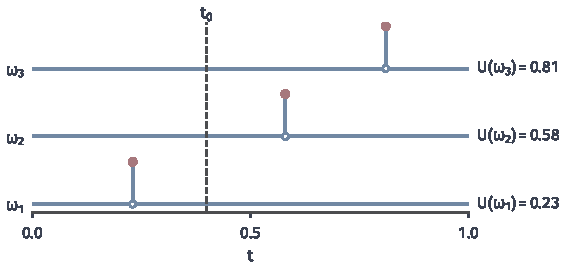
\includegraphics[width=96mm]{figures/07-probability/02-measure-theoretic-probability/matplotlib/pspace-uncountable-spikes/figure.pdf}
  \caption{$X_t=\mathbf{1}_{\{U=t\}}$在三个样本点上的取值，横轴是$t$。每条蓝线只在$t=U(\omega)$处跳到$1$（红点）。虚线是固定时刻$t_0$，它碰到尖峰的概率为零；然而每个样本点的曲线都有一个尖峰。}
  \label{fig:pspace-uncountable-spikes}
\end{BookInlineFigure}

要从“每个$t$几乎必然”推出“几乎必然对一切$t$”，需要额外的结构。例如，若已知每条曲线$t\mapsto X_t(\omega)$都连续，就只需检查可数个有理数时刻：它们在零概率事件之外同时为零，连续性再把结论推到所有$t$。上面的$X_t$不连续，这条路走不通。以连续时间为指标的随机对象经常遇到这个问题，本章只处理可数个陈述。

\subsection{完备化}
\label{sec:pspace-completion}

几乎必然的陈述允许在零概率事件上随意修改。修改以后的对象还在原来的事件族里吗？先看一个小例子。

\paragraph{修改可能破坏可测性}
取$\Omega=\{1,2,3\}$，事件族与概率为
\[
  \mathcal{F}=\bigl\{\varnothing,\{1\},\{2,3\},\Omega\bigr\},\qquad \mathbb{P}(\{1\})=1,\quad \mathbb{P}(\{2,3\})=0 .
\]这个事件族只能区分“结果是$1$”与“结果在$\{2,3\}$中”。按卷四的说法，函数$X:\Omega\to\mathbb{R}$\emph{可测}是指对每个Borel集$B$，$\{X\in B\}\in\mathcal{F}$；第~\ref{sec:pspace-random-objects}节将把这样的函数称为随机变量。

$X\equiv0$可测，因为它的每个原像都是$\varnothing$或$\Omega$。令$X'=\mathbf{1}_{\{2\}}$，它与$X$只在点$2$不同，而$\{2\}\subseteq\{2,3\}$包含于零概率事件，所以$X'=X$几乎必然成立。然而$\{X'=1\}=\{2\}\notin\mathcal{F}$，$X'$不可测。两个函数几乎必然相等，一个可测、一个不可测，问题出在$\mathcal{F}$不含零概率事件$\{2,3\}$的子集。

\paragraph{完备化的定义}
卷四的完备化正好补上这些集合。称概率空间$(\Omega,\mathcal{F},\mathbb{P})$\term{完备概率空间}（complete probability space），若每个零概率事件的每个子集都属于$\mathcal{F}$。对任意概率空间，令
\begin{equation}
  \overline{\mathcal{F}}=\{A\cup M:\ A\in\mathcal{F},\ M\subseteq N\text{ 对某个零概率事件 }N\},\qquad \overline{\mathbb{P}}(A\cup M)=\mathbb{P}(A).
  \label{eq:pspace-completion}
\end{equation}
卷四证明了：$\overline{\mathcal{F}}$是包含$\mathcal{F}$的$\sigma$代数，$\overline{\mathbb{P}}$与表示方式无关，是$\overline{\mathcal{F}}$上的概率测度，在$\mathcal{F}$上与$\mathbb{P}$一致，并且$(\Omega,\overline{\mathcal{F}},\overline{\mathbb{P}})$完备。

在上面的例子中，零概率事件只有$\varnothing$和$\{2,3\}$，它们的子集$\{2\}$、$\{3\}$被补入，再与$\{1\}$取并，得到全部$8$个子集（图~\ref{fig:pspace-completion}）。新补入的事件中，含点$1$的概率为$1$，不含点$1$的概率为$0$；原有$4$个事件的概率不变。

\begin{BookInlineFigure}
  \centering
  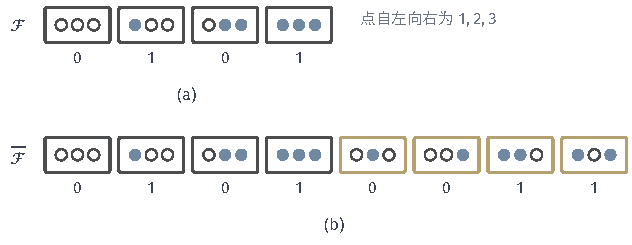
\includegraphics[width=107mm]{figures/07-probability/02-measure-theoretic-probability/tikz/pspace-completion/figure.pdf}
  \caption{三点样本空间的完备化。每个方框是一个事件，实心点表示该点属于事件，下方数字是概率。(a)原事件族$\mathcal{F}$只有$4$个事件；(b)完备化补入零概率事件$\{2,3\}$的子集及其与$\{1\}$的并（黄框），共$8$个事件，原有事件的概率不变。}
  \label{fig:pspace-completion}
\end{BookInlineFigure}

\paragraph{完备空间中的修改}
在完备的概率空间里，零概率事件上的修改不会破坏可测性。

\begin{theorem}[零概率修改保持可测性]
\label{thm:pspace-modification}
设$(\Omega,\mathcal{F},\mathbb{P})$完备，$X:\Omega\to\mathbb{R}$可测，$X':\Omega\to\mathbb{R}$满足：存在零概率事件$N$，使得在$N$之外$X'=X$。则$X'$可测，且对每个Borel集$B$，
\begin{equation}
  \mathbb{P}(X'\in B)=\mathbb{P}(X\in B).
  \label{eq:pspace-modification}
\end{equation}
\end{theorem}

\begin{proof}
把$\{X'\in B\}$按是否落在$N$中分成两块：
\[
  \{X'\in B\}=\bigl(\{X\in B\}\cap N^{\mathrm{c}}\bigr)\cup\bigl(\{X'\in B\}\cap N\bigr).
\]
在$N^{\mathrm{c}}$上$X'=X$，所以第一块等于$\{X\in B\}\cap N^{\mathrm{c}}$，它是两个事件之交，属于$\mathcal{F}$。第二块包含于零概率事件$N$，由完备性也属于$\mathcal{F}$，且概率为零。所以$\{X'\in B\}\in\mathcal{F}$，并且
\[
  \mathbb{P}(X'\in B)=\mathbb{P}\bigl(\{X\in B\}\cap N^{\mathrm{c}}\bigr)=\mathbb{P}(X\in B),
\]
最后一步是因为$\{X\in B\}$与$\{X\in B\}\cap N^{\mathrm{c}}$相差的部分包含于$N$。
\end{proof}

木棍上的随机点就有这样的例子。卷四指出，$\mathcal{B}([0,1))$关于长度的完备化是Lebesgue可测集族。Cantor集的长度为零，在完备化后它的每个子集都是事件，概率都是零，其中包括不是Borel集的子集。于是，把一个随机变量在Cantor集的任意子集上改掉，得到的函数在完备空间中仍然可测，所有概率都不变。

\paragraph{完备化不做的事}
完备化只是把“包含于零概率事件”的集合补进来并赋予概率零，它不改变原有事件的概率，也不会让任何零概率事件变成正概率事件。特别地，它不能帮助我们以零概率事件为条件。给定$U=1/2$时某事件的条件概率，按第~\ref{chap:classical-probability}章的定义是
\[
  \mathbb{P}(A\mid U=1/2)=\frac{\mathbb{P}(A\cap\{U=1/2\})}{\mathbb{P}(U=1/2)},
\]
分母为零，完备化前后都一样。给定连续观测值求条件规律，要用第~\ref{chap:conditional-expectation}章和第~\ref{chap:conditional-distributions}章的办法。

完备化也有代价。零概率事件依赖于概率测度，对一个测度完备的事件族，换一个测度就未必完备；同时讨论多个概率测度时，通常保留原来的事件族。对取值空间，惯例是使用Borel $\sigma$代数而不完备化：卷四说明过，Lebesgue可测函数与连续函数的复合未必Lebesgue可测，取值一侧若换成更大的事件族，复合运算就可能失去可测性。本章约定：样本空间一侧需要时可以完备化，取值空间一律使用Borel $\sigma$代数。

\section{随机对象}
\label{sec:pspace-random-objects}

第~\ref{chap:random-variables}章把随机变量定义为样本空间上的实值函数，并直接对$\{X\in B\}$谈概率。那时事件族是全部子集或者只涉及区间，$\{X\in B\}$是否为事件不成问题。现在事件族是指定的$\mathcal{F}$，一个函数的原像未必落在$\mathcal{F}$里；而我们还会观测向量、矩阵、图这样的对象。什么样的函数才配称为随机变量？

\paragraph{可测性：观测引出的问题都有概率}
回到只知道点数和的观察者，他的事件族是$\sigma(S)$。若他想研究第一枚骰子的点数$X_1$，就会遇到$\{X_1=1\}\notin\sigma(S)$：这个“随机变量”提出的问题，他的事件族无法回答。所以随机变量的定义必须保证，凡是由它引出的“取值落在某个集合中”的问题，答案都在事件族里。卷四的可测映射正是这个要求。

\begin{definition}[随机对象与随机变量]
\label{def:pspace-random-object}
设$(\Omega,\mathcal{F},\mathbb{P})$是概率空间，$(E,\mathcal{E})$是可测空间。映射$X:\Omega\to E$若满足
\begin{equation}
  X^{-1}(B)=\{\omega\in\Omega:X(\omega)\in B\}\in\mathcal{F},\qquad B\in\mathcal{E},
  \label{eq:pspace-measurable}
\end{equation}
则称$X$为取值于$E$的\term{随机对象}（random element）。取值于$(\mathbb{R},\mathcal{B}(\mathbb{R}))$的随机对象称为随机变量，取值于$(\mathbb{R}^{d},\mathcal{B}(\mathbb{R}^{d}))$的称为$d$维随机向量。
\end{definition}

图~\ref{fig:pspace-random-object-map}画出了这个定义。$X$把$\Omega$中的点送到$E$中；对$E$中的集合$B$，把所有被送进$B$的样本点收集起来，就是原像$X^{-1}(B)$。这个原像可以由几块分开的区域组成，可测性要求它是事件，从而有概率。

\begin{BookInlineFigure}
  \centering
  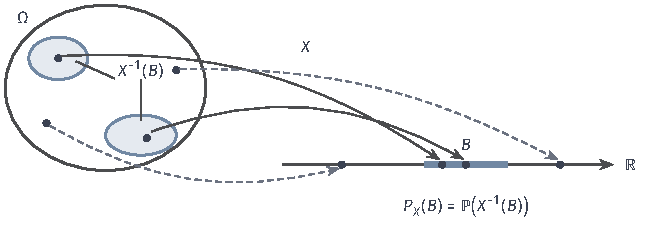
\includegraphics[width=110mm]{figures/07-probability/02-measure-theoretic-probability/tikz/pspace-random-object-map/figure.pdf}
  \caption{随机变量$X:\Omega\to\mathbb{R}$与原像。实线箭头把浅蓝的两块区域中的点送进集合$B$（粗蓝线段），虚线箭头把其他点送到$B$之外。$X^{-1}(B)$是两块区域之并，可测性要求它是事件，它的概率就是取值落在$B$中的概率。}
  \label{fig:pspace-random-object-map}
\end{BookInlineFigure}

定义要求对$\mathcal{E}$中\emph{每个}集合检查原像，实际操作时只需检查一个生成族。卷四的生成族判据说：若$\mathcal{E}=\sigma(\mathcal{C})$，则$X$可测当且仅当对每个$C\in\mathcal{C}$都有$X^{-1}(C)\in\mathcal{F}$。原因是原像运算与补集、可数并交换，使得原像为事件的集合$B$构成一个$\sigma$代数，它包含$\mathcal{C}$，也就包含$\sigma(\mathcal{C})$。对实值函数，取半直线为生成族，得到常用的判别：
\begin{equation}
  X\text{ 是随机变量}\iff\{X\leq x\}\in\mathcal{F}\quad\text{对一切 }x\in\mathbb{R}.
  \label{eq:pspace-rv-criterion}
\end{equation}

\paragraph{常见的取值空间}
映射$\bm{X}=(X_1,\dots,X_d):\Omega\to\mathbb{R}^{d}$是随机向量，当且仅当每个坐标$X_i$都是随机变量。一方面，坐标投影连续，因而Borel可测，可测映射的复合仍可测。另一方面，$\mathcal{B}(\mathbb{R}^{d})$由左下象限生成，而
\[
  \{\bm{X}\in(-\infty,x_1]\times\cdots\times(-\infty,x_d]\}=\bigcap_{i=1}^{d}\{X_i\leq x_i\}
\]
是$d$个事件之交。所以第~\ref{chap:random-vectors}章逐个坐标定义的随机向量，正好是这里的$\mathbb{R}^{d}$值随机对象。

随机矩阵可以看成拉直的向量。把$m\times n$实矩阵按元素排成$\mathbb{R}^{mn}$中的向量，$\mathbb{R}^{m\times n}$就带有Borel $\sigma$代数，随机矩阵$\bm{M}$可测当且仅当每个元素$M_{i,j}$都是随机变量。例如随机向量$\bm{X}$的外积$\bm{X}\bm{X}^{\top}$，其元素$X_iX_j$是随机变量的乘积，所以它是随机矩阵。

有限集合是另一类常见的取值空间，配上全部子集作为事件族。这时可测性只需检查单点：$X$可测当且仅当对每个可能的取值$g$，$\{X=g\}\in\mathcal{F}$，因为任何子集都是有限个单点之并。

\paragraph{有限随机图}
以$3$个带标号顶点上的随机图为例。$3$个顶点之间有$3$条可能的边，每条边出现与否用一个比特记录，样本空间是$\Omega=\{0,1\}^{3}$，取全部子集为事件族，并让$8$个结果等可能。映射$G$把结果$\omega=(e_{1,2},e_{1,3},e_{2,3})$送到边集为$\{\{i,j\}:e_{i,j}=1\}$的图。取值空间$E$是这$3$个顶点上全部$2^{3}=8$个图，同样取全部子集。

在这个模型里$\Omega$与$E$一一对应，可测性不成问题。值得注意的是由图算出的数值。边数$N=e_{1,2}+e_{1,3}+e_{2,3}$是$E$上函数与$G$的复合，它把$8$个图分成$4$组（图~\ref{fig:pspace-random-graph}），由此得到
\[
  \mathbb{P}(N=0)=\tfrac18,\quad \mathbb{P}(N=1)=\tfrac38,\quad \mathbb{P}(N=2)=\tfrac38,\quad \mathbb{P}(N=3)=\tfrac18 .
\]
“图是三角形”是事件$\{N=3\}$，“图连通”是$\{N\geq2\}$，因为$3$个顶点上的图连通当且仅当至少有$2$条边。

\begin{BookInlineFigure}
  \centering
  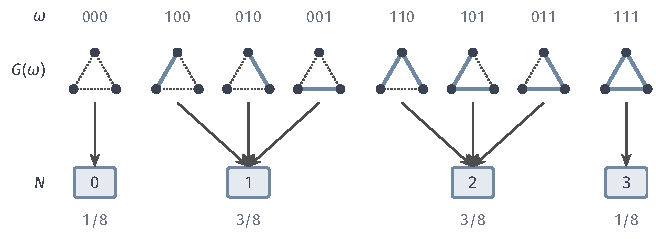
\includegraphics[width=111mm]{figures/07-probability/02-measure-theoretic-probability/tikz/pspace-random-graph/figure.pdf}
  \caption{$3$个顶点上的随机图。上行是结果$\omega=(e_{1,2},e_{1,3},e_{2,3})$，中间是对应的图$G(\omega)$，蓝色实线是出现的边，点线是未出现的边；顶点$1$在上，$2$在左下，$3$在右下。边数$N$把$8$个等可能的图分成$4$组，下方是各组的概率。}
  \label{fig:pspace-random-graph}
\end{BookInlineFigure}

更大的随机图也一样：$n$个顶点有$n(n-1)/2$条可能的边，取值空间有$2^{n(n-1)/2}$个图。边数、三角形个数、最大度数、是否连通，都是有限集合上的函数，与$G$复合后自动成为随机变量。一般地，若$X$是取值于$(E,\mathcal{E})$的随机对象，$g:E\to E'$是可测映射，则对$B\in\mathcal{E}'$，
\[
  (g\circ X)^{-1}(B)=X^{-1}\bigl(g^{-1}(B)\bigr)\in\mathcal{F},
\]
因为$g^{-1}(B)\in\mathcal{E}$。所以$g(X)$也是随机对象。连续函数关于Borel $\sigma$代数可测，于是随机向量的和、积、范数，随机对称矩阵的迹，都是随机变量。

\paragraph{观测生成的事件族}
可测性说明观测\emph{不超出}事件族的回答能力。反过来也可以问：一个观测本身能回答哪些问题？观测$X$之后，对每个$B\in\mathcal{E}$，我们都能判断$X\in B$是否成立，也就是判断事件$X^{-1}(B)$是否发生。这些事件收集起来，就是$X$提供的信息。

\begin{definition}[观测生成的$\sigma$代数]
\label{def:pspace-generated-sigma}
设$X:\Omega\to E$是取值于$(E,\mathcal{E})$的随机对象。称
\begin{equation}
  \sigma(X)=\bigl\{X^{-1}(B):\ B\in\mathcal{E}\bigr\}
  \label{eq:pspace-generated-sigma}
\end{equation}
为$X$\term{生成的$\sigma$代数}（$\sigma$-algebra generated by $X$）。对多个随机对象$X_1,\dots,X_n$，$\sigma(X_1,\dots,X_n)$指向量$(X_1,\dots,X_n)$生成的$\sigma$代数。
\end{definition}

$\sigma(X)$确实是$\sigma$代数：$X^{-1}(E)=\Omega$，并且原像与补集、可数并交换，
\[
  \bigl(X^{-1}(B)\bigr)^{\mathrm{c}}=X^{-1}(B^{\mathrm{c}}),\qquad \bigcup_{k}X^{-1}(B_k)=X^{-1}\Bigl(\bigcup_kB_k\Bigr).
\]
它包含于$\mathcal{F}$，这就是可测性。它也是使$X$可测的最小$\sigma$代数：任何使$X$可测的$\sigma$代数都必须含有全部原像$X^{-1}(B)$。

当$X$只取有限个值时，$\sigma(X)$的原子就是$X$的各个等值集$\{X=x\}$，事件是若干等值集之并。第~\ref{sec:pspace-events}节的“只知道点数和”就是$\sigma(S)$，它的原子是$11$条反对角线；“只知道较大点数”就是$\sigma(M)$，原子是$6$个L形区域。只知道“点数和是否为$7$”，对应的是指示变量$\mathbf{1}_{\{S=7\}}$，它生成的$\sigma$代数只有$4$个事件。

\paragraph{函数只会减少信息}
对观测结果再作变换，信息不会增加。设$g$可测，对$B\in\mathcal{E}'$，
\[
  \bigl(g(X)\bigr)^{-1}(B)=X^{-1}\bigl(g^{-1}(B)\bigr)\in\sigma(X),
\]
所以$\sigma(g(X))\subseteq\sigma(X)$。在骰子的例子里，$\mathbf{1}_{\{S=7\}}$是$S$的函数，$\sigma(\mathbf{1}_{\{S=7\}})\subseteq\sigma(S)$：知道点数和就知道它是否为$7$，反之不行。若$g$是双向可测的一一映射，两个方向都用上述包含关系，得到$\sigma(g(X))=\sigma(X)$：可逆的重新编码不改变信息。

木棍上的随机点给出一串逐渐精细的观测。设$\Omega=[0,1)$，$\omega$的二进制展开为$0.D_1D_2D_3\cdots$，取不以无穷个$1$结尾的那种展开，即
\[
  D_k(\omega)=\lfloor2^{k}\omega\rfloor-2\lfloor2^{k-1}\omega\rfloor\in\{0,1\}.
\]
记$K=\lfloor4\omega\rfloor$，它告诉我们$\omega$落在哪个四分之一区间。图~\ref{fig:pspace-nested-information}列出了几个观测的原子。$D_1=\lfloor K/2\rfloor$与$D_2=K-2D_1$都是$K$的函数，所以$\sigma(D_1)$和$\sigma(D_2)$都包含于$\sigma(K)$；$K$又是$\lfloor8\omega\rfloor$的函数。$\sigma(D_2)$的一个原子是$[1/4,1/2)\cup[3/4,1)$，由两段不相邻的区间组成，它说明粗信息未必是“把区间分得粗一点”。$\sigma(D_1)$与$\sigma(D_2)$互不包含，两者合起来恰好是$\sigma(K)$。

\begin{BookInlineFigure}
  \centering
  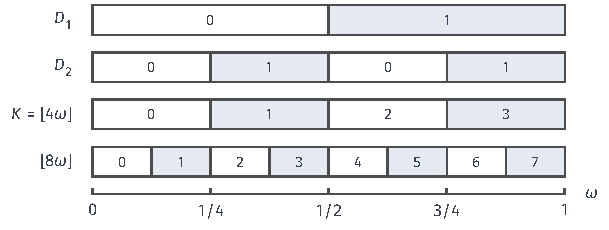
\includegraphics[width=103mm]{figures/07-probability/02-measure-theoretic-probability/tikz/pspace-nested-information/figure.pdf}
  \caption{$\Omega=[0,1)$上几个观测生成的原子。每一行把$[0,1)$分成若干格，格内数字是该观测的取值，浅蓝格子取奇数值。$D_1$、$D_2$是前两位二进制数字，$K=\lfloor4\omega\rfloor$。$\sigma(D_1)$与$\sigma(D_2)$都包含于$\sigma(K)$，$\sigma(K)$又包含于$\sigma(\lfloor8\omega\rfloor)$；$D_2$的原子各由两段不相邻的区间组成。}
  \label{fig:pspace-nested-information}
\end{BookInlineFigure}

观测$X(\omega)=\omega$本身生成全部Borel集，它提供完整的信息。这里讨论的都是一次观测，或同时取得的有限个观测。信息随时间逐步增加、后一时刻知道得比前一时刻多的情形，要用一列递增的$\sigma$代数描述，属于随机过程的内容。第~\ref{chap:conditional-expectation}章将以$\sigma(X)$为“已知信息”，研究给定信息后怎样求平均。

\section{分布与推前}
\label{sec:pspace-distributions}

随机变量是样本空间上的函数，可是多数问题只关心它的取值落在哪里、各处概率多大，并不关心是哪个样本点产生了这个取值。第~\ref{chap:random-variables}章把这种“取值的规律”称为分布，并只对区间及其有限并计算过它。现在把分布定义为取值空间上的一个完整的概率测度。

\paragraph{分布的定义}
随机对象$X$把每个样本点$\omega$送到$E$中的点$X(\omega)$。把$\omega$所带的概率质量随之搬过去，$E$中集合$B$所收到的质量，就是被送进$B$的那些样本点的质量之和，即$\mathbb{P}(X^{-1}(B))$。

\begin{definition}[分布]
\label{def:pspace-distribution}
设$X$是取值于$(E,\mathcal{E})$的随机对象。称
\begin{equation}
  P_X(B)=\mathbb{P}\bigl(X^{-1}(B)\bigr)=\mathbb{P}(X\in B),\qquad B\in\mathcal{E},
  \label{eq:pspace-distribution}
\end{equation}
为$X$的分布。$P_X$是$\mathbb{P}$在$X$下的推前测度，也记作$\mathbb{P}\circ X^{-1}$。
\end{definition}

$P_X$是$(E,\mathcal{E})$上的概率测度。总质量$P_X(E)=\mathbb{P}(\Omega)=1$；若$B_1,B_2,\dots$两两不交，它们的原像也两两不交，并且原像之并等于并集的原像，于是由$\mathbb{P}$的可数可加性，
\[
  P_X\Bigl(\bigcup_kB_k\Bigr)=\mathbb{P}\Bigl(\bigcup_kX^{-1}(B_k)\Bigr)=\sum_k\mathbb{P}\bigl(X^{-1}(B_k)\bigr)=\sum_kP_X(B_k).
\]
推前测度的一般理论，包括映射下的密度公式，可参考\BookChapterRef{chap:pushforward-measures}{卷四第9章“推前测度”}。

有了$P_X$，关于$X$取值的问题都可以在$(E,\mathcal{E},P_X)$上回答，不必再回到$\Omega$。第~\ref{chap:random-variables}章说“取值集合可以当作新的样本空间”，现在有了准确的含义：$(E,\mathcal{E},P_X)$本身就是一个概率空间。

\paragraph{用原像计算分布}
在木棍模型$\Omega=[0,1)$上定义$X(\omega)=-\ln(1-\omega)$。$X$连续且严格递增，从$0$增加到$+\infty$，因而是随机变量。对$x\geq0$，$X>x$等价于$\omega>1-\mathrm{e}^{-x}$，所以
\[
  \mathbb{P}(X>x)=\lambda\bigl((1-\mathrm{e}^{-x},1)\bigr)=\mathrm{e}^{-x}.
\]
这正是$\operatorname{Exp}(1)$的右尾概率：均匀的质量经过$X$的搬运，变成了指数分布。

用同一个原像规则可以算任何区间的概率。取$B=(1,2]$，它的原像是$\omega$轴上的区间$(1-\mathrm{e}^{-1},1-\mathrm{e}^{-2}]$，于是
\[
  P_X\bigl((1,2]\bigr)=(1-\mathrm{e}^{-2})-(1-\mathrm{e}^{-1})=\mathrm{e}^{-1}-\mathrm{e}^{-2}\approx0.2325 .
\]
图~\ref{fig:pspace-pushforward-exp}(a)把这个原像画了出来：纵轴上的$B$经曲线反射到横轴，得到长约$0.865-0.632$的区间。图~\ref{fig:pspace-pushforward-exp}(b)是同一概率在取值空间上的样子，即指数密度在$(1,2]$上的面积。

\begin{BookInlineFigure}
  \centering
  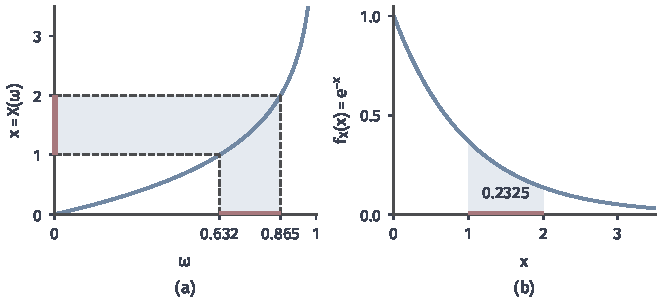
\includegraphics[width=112mm]{figures/07-probability/02-measure-theoretic-probability/matplotlib/pspace-pushforward-exp/figure.pdf}
  \caption{用原像计算推前分布。(a)蓝线是$x=X(\omega)=-\ln(1-\omega)$，纵轴上的红色线段是$B=(1,2]$，它的原像是横轴上的红色线段$(0.632,0.865]$，长度$\mathrm{e}^{-1}-\mathrm{e}^{-2}$；(b)取值空间上的分布，浅蓝面积是$P_X((1,2])\approx0.2325$。}
  \label{fig:pspace-pushforward-exp}
\end{BookInlineFigure}

对实值随机变量，分布函数$F_X(x)=P_X((-\infty,x])$就是式~\eqref{eq:pspace-cdf}对$P=P_X$的特例。由定理~\ref{thm:pspace-cdf-measure}，$F_X$确定了整个$P_X$：两个随机变量的分布函数相同，它们落在任何Borel集中的概率都相同。第~\ref{chap:random-variables}章只能从分布函数读出区间的概率，这一缺口现在补上了。

\paragraph{变换后的分布}
对随机对象再作可测变换$Y=g(X)$，$Y$的分布可以只用$X$的分布算出。对$B\in\mathcal{E}'$，$\{Y\in B\}=\{X\in g^{-1}(B)\}$，所以
\begin{equation}
  P_{g(X)}(B)=P_X\bigl(g^{-1}(B)\bigr).
  \label{eq:pspace-transform-law}
\end{equation}
质量先由$X$从$\Omega$搬到$E$，再由$g$从$E$搬到$E'$，两次搬运的结果与一次搬运$g\circ X$相同。

截断的等待时间是一个例子。对指数变量$X$取$Y=\min\{X,2\}$，即$g(x)=\min\{x,2\}$。单点$\{2\}$的原像是$[2,\infty)$，由式~\eqref{eq:pspace-transform-law}，
\[
  P_Y(\{2\})=P_X\bigl([2,\infty)\bigr)=\mathrm{e}^{-2}\approx0.1353,
\]
而$y<2$时$P_Y((-\infty,y])=P_X((-\infty,y])$。$X$在$[2,\infty)$上的质量全部被搬到点$2$上，所以$Y$的分布在$2$处有一个原子，这就是第~\ref{chap:random-variables}章在分布函数上看到的跳跃。第~\ref{chap:random-variable-transformations}章的各种换元公式，都是在具体的$g$下计算式~\eqref{eq:pspace-transform-law}；离散、连续和混合的情形使用的是同一条原像规则。

\paragraph{任何分布函数都可以实现}
定理~\ref{thm:pspace-cdf-measure}在实轴上造出了以$F$为分布函数的概率测度。能否在某个概率空间上造出一个随机变量，使它的分布函数恰好是$F$？最直接的办法是把$(\mathbb{R},\mathcal{B}(\mathbb{R}),P)$本身当作样本空间，令$X(x)=x$。下面给出另一种构造，它只用木棍上的一个均匀点，后面构造独立序列时会反复用到。

对满足定理~\ref{thm:pspace-cdf-measure}条件的$F$，定义
\begin{equation}
  Q(u)=\inf\{x\in\mathbb{R}:\ F(x)\geq u\},\qquad 0<u<1 .
  \label{eq:pspace-quantile}
\end{equation}
这就是第~\ref{chap:random-variables}章的分位数函数。$0<u<1$保证集合$\{x:F(x)\geq u\}$非空（因为$F\to1$）且有下界（因为$F\to0$），所以$Q(u)$是有限实数。

\begin{lemma}[分位数函数的基本关系]
\label{lem:pspace-quantile}
对$0<u<1$与$x\in\mathbb{R}$，
\begin{equation}
  Q(u)\leq x\iff u\leq F(x).
  \label{eq:pspace-quantile-galois}
\end{equation}
\end{lemma}

\begin{proof}
若$u\leq F(x)$，则$x$属于集合$\{y:F(y)\geq u\}$，下确界不超过它，即$Q(u)\leq x$。

反过来，先证下确界本身属于这个集合。取集合中的一列点$y_n\downarrow Q(u)$，每个都满足$F(y_n)\geq u$。由右连续性，
\[
  F\bigl(Q(u)\bigr)=\lim_{n\to\infty}F(y_n)\geq u .
\]
于是若$Q(u)\leq x$，由$F$单调不减得$F(x)\geq F(Q(u))\geq u$。
\end{proof}

\begin{theorem}[分位数变换]
\label{thm:pspace-quantile-transform}
设$F$满足定理~\ref{thm:pspace-cdf-measure}的条件，$Q$由式~\eqref{eq:pspace-quantile}定义。在$\Omega=[0,1)$、$\mathcal{F}=\mathcal{B}([0,1))$、$\mathbb{P}=\lambda$上，令$X(\omega)=Q(\omega)$（$\omega>0$），$X(0)=0$。则$X$是随机变量，且$F_X=F$。
\end{theorem}

\begin{proof}
对$x\in\mathbb{R}$，由式~\eqref{eq:pspace-quantile-galois}，
\[
  \{\omega\in(0,1):X(\omega)\leq x\}=\{\omega\in(0,1):\omega\leq F(x)\}=(0,F(x)]\cap(0,1).
\]
$\{X\leq x\}$是这个区间与可能的单点$\{0\}$之并，是Borel集，由判别~\eqref{eq:pspace-rv-criterion}，$X$是随机变量。单点概率为零，所以
\[
  \mathbb{P}(X\leq x)=\lambda\bigl((0,F(x)]\cap(0,1)\bigr)=F(x),
\]
最后一步在$F(x)=1$时也成立，因为$(0,1)$的长度是$1$。
\end{proof}

用等待时间$W$走一遍。分布函数在$t\geq0$时为$F_W(t)=0.3+0.7(1-\mathrm{e}^{-t})$，在$0$处从$0$跳到$0.3$。由式~\eqref{eq:pspace-quantile}，$u\leq0.3$时最小的满足$F_W(x)\geq u$的点是$0$；$u>0.3$时解方程$F_W(x)=u$。于是
\begin{equation}
  Q_W(u)=\begin{cases}0,&0<u\leq0.3,\\ \ln\dfrac{0.7}{1-u},&0.3<u<1.\end{cases}
  \label{eq:pspace-waiting-quantile}
\end{equation}
取两个均匀随机数$u=0.2$与$u=0.37$，得到
\[
  Q_W(0.2)=0,\qquad Q_W(0.37)=\ln\frac{0.7}{0.63}=\ln\frac{10}{9}\approx0.1054 .
\]
第一个落在跳跃的高度范围内，对应“不用等”；第二个对应等待约$0.105$个单位时间。图~\ref{fig:pspace-quantile-transform}显示，分布函数在$0$处的跳跃，变成了分位数函数在$(0,0.3]$上的平台：长度为$0.3$的一段均匀质量全部被送到点$0$。

\begin{BookInlineFigure}
  \centering
  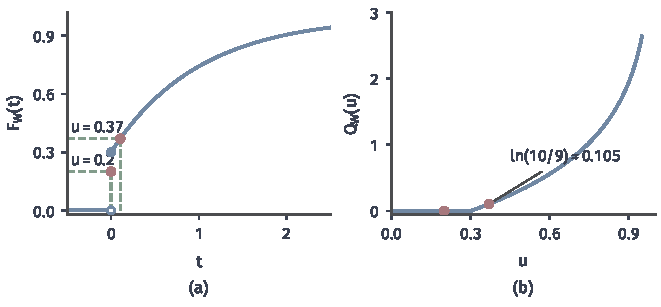
\includegraphics[width=112mm]{figures/07-probability/02-measure-theoretic-probability/matplotlib/pspace-quantile-transform/figure.pdf}
  \caption{用分位数变换从均匀随机数得到等待时间$W$。(a)蓝线是$F_W$；绿色虚线从高度$u$水平向右，碰到曲线（或跳跃的竖直段）后竖直向下，落点就是$Q_W(u)$；$u=0.2$落在跳跃内，得到$0$，$u=0.37$得到$\ln(10/9)$。(b)蓝线是$Q_W$，它在$(0,0.3]$上为$0$，红点是两个例子。}
  \label{fig:pspace-quantile-transform}
\end{BookInlineFigure}

定理~\ref{thm:pspace-quantile-transform}对Cantor分布同样适用，于是Cantor变量可以由一个均匀随机点得到。它也是从均匀随机数生成任意一维分布样本的基本方法，第~\ref{chap:sample-generation}章将讨论它的计算问题。

\paragraph{三种相等}
两个随机变量“相同”可以有三种不同强度的意思。设$X,Y$是同一概率空间上的随机变量。若对每个$\omega$都有$X(\omega)=Y(\omega)$，称它们处处相等；若$\mathbb{P}(X=Y)=1$，称它们几乎必然相等。第三种只比较分布，两个变量甚至可以定义在不同的概率空间上。

\begin{definition}[同分布]
\label{def:pspace-equal-in-law}
若随机对象$X$与$Y$取值于同一可测空间，且$P_X=P_Y$，则称$X$与$Y$同分布，记作
\begin{equation}
  X\overset{\mathrm{d}}{=}Y .
  \label{eq:pspace-equal-in-law}
\end{equation}
\end{definition}

三者依次减弱。处处相等时$\{X\neq Y\}=\varnothing$，所以处处相等蕴含几乎必然相等。若$X=Y$几乎必然成立，记$N=\{X\neq Y\}$，则对每个Borel集$B$，$\{X\in B\}$与$\{Y\in B\}$只在$N$中可能不同，它们的对称差包含于$N$，所以
\[
  \bigl\lvert P_X(B)-P_Y(B)\bigr\rvert\leq\mathbb{P}(N)=0,
\]
即$X\overset{\mathrm{d}}{=}Y$。

反方向都不成立。在木棍模型上取$U(\omega)=\omega$与$1-U$。对$u\in[0,1)$，
\[
  \mathbb{P}(1-U\leq u)=\mathbb{P}(U\geq1-u)=u,
\]
所以$1-U$也是均匀分布，$U\overset{\mathrm{d}}{=}1-U$。可是$U=1-U$只在$\omega=1/2$成立，$\mathbb{P}(U=1-U)=0$：两个同分布的变量几乎处处不相等，见图~\ref{fig:pspace-three-equalities}(a)。另一方面，把$U$在可数个点上改成$0$得到$U'$，例如在$\omega=k/8$（$k=1,\dots,7$）处，则$U'\neq U$只在一个零概率事件上发生，$U'=U$几乎必然成立，却不处处成立，见图~\ref{fig:pspace-three-equalities}(b)。

\begin{BookInlineFigure}
  \centering
  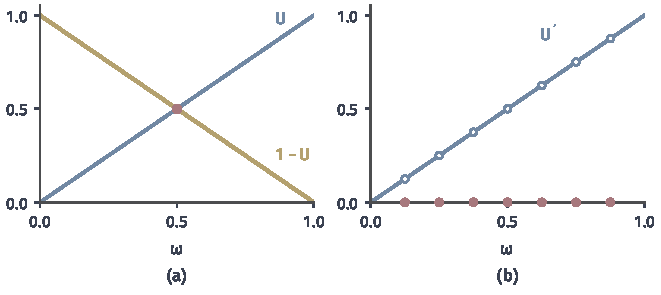
\includegraphics[width=112mm]{figures/07-probability/02-measure-theoretic-probability/matplotlib/pspace-three-equalities/figure.pdf}
  \caption{三种相等的区别，横轴是样本点$\omega\in[0,1)$。(a)蓝线$U(\omega)=\omega$与黄线$1-U$只在红点$\omega=1/2$处相等，二者却同为均匀分布；(b)$U'$在$\omega=k/8$处被改为$0$（红点），空心点是原来的值，其余位置与$U$相同，二者几乎必然相等。}
  \label{fig:pspace-three-equalities}
\end{BookInlineFigure}

这三种相等在实践中各有用处。一切只依赖分布的量，例如$\mathbb{P}(X>2)$、分位数以及第~\ref{sec:pspace-expectation}节将统一定义的期望，对同分布的变量都相同。几乎必然相等的变量还能在同一个样本点上互相替换，这在讨论多个变量的组合时是必需的。处处相等很少需要，因为零概率事件上的差别不影响任何概率。

\paragraph{边缘分布不能确定配对}
同分布的变量不能随意替换进组合中。仍取$X=U$与$X'=1-U$，二者同分布；再取$Y=U$，则
\[
  X+Y=2U,\qquad X'+Y=1 .
\]
前者均匀分布在$[0,2)$上，后者恒等于$1$。原因是$X+Y$的分布不只依赖$X$和$Y$各自的分布，还依赖它们在同一个样本点上怎样配对。

配对由联合分布描述。$(X,Y)$是取值于$\mathbb{R}^{2}$的随机向量，它的分布$P_{(X,Y)}$称为联合分布；$X$的分布是它在坐标投影$\pi_1(x,y)=x$下的推前，
\[
  P_X(B)=\mathbb{P}\bigl((X,Y)\in B\times\mathbb{R}\bigr)=P_{(X,Y)}\bigl(\pi_1^{-1}(B)\bigr).
\]
差$X-Y$是映射$(x,y)\mapsto x-y$下的推前，所以它的分布由联合分布确定，却不能由两个边缘分布确定。

下面三种配对的边缘都是$[0,1)$上的均匀分布：$(U,U)$、$(U,1-U)$，以及$(U,V)$，其中$V$是与$U$独立的另一个均匀变量（第~\ref{sec:pspace-independence}节在同一个概率空间上构造它）。记$D=X-Y$，三种配对下：
\begin{enumerate}
  \item $(U,U)$：$D\equiv0$，质量全部集中在原点；
  \item $(U,1-U)$：$D=2U-1$，均匀分布在$(-1,1)$上，密度为$1/2$；
  \item $(U,V)$：$D$的密度是$1-\lvert z\rvert$（$\lvert z\rvert<1$），即第~\ref{chap:random-variable-transformations}章算过的三角形密度。
\end{enumerate}
差的大小随配对变化很大。以$\mathbb{P}(\lvert D\rvert\leq0.1)$为例，三种配对依次是
\[
  1,\qquad \frac{0.2}{2}=0.1,\qquad 1-0.9^{2}=0.19 .
\]
第三个数是三角形密度在$[-0.1,0.1]$上的积分，等于$1$减去两侧两个直角三角形的面积$2\times\frac12\times0.9^{2}$。$D$的方差依次为$0$、$1/3$和$1/6$。

\begin{BookInlineFigure}
  \centering
  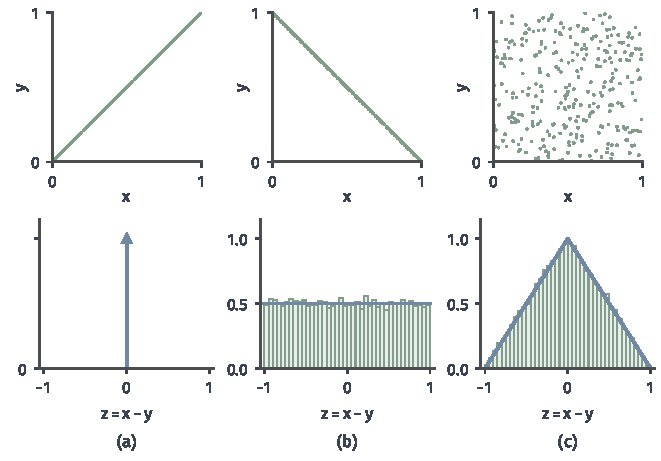
\includegraphics[width=112mm]{figures/07-probability/02-measure-theoretic-probability/matplotlib/pspace-couplings/figure.pdf}
  \caption{三种边缘相同的配对。上行是$300$对模拟样本（种子$9$）的散点：(a)$(U,U)$落在对角线上，(b)$(U,1-U)$落在反对角线上，(c)独立的$(U,V)$铺满正方形。下行是$D=X-Y$的分布：(a)全部质量在$0$（箭头表示单点质量$1$），(b)(c)中浅绿直方图来自$20000$对模拟样本，蓝线分别是均匀密度$1/2$与三角形密度$1-\lvert z\rvert$。}
  \label{fig:pspace-couplings}
\end{BookInlineFigure}

图~\ref{fig:pspace-couplings}的上行显示，三种配对的质量在平面上的位置完全不同，但向两条坐标轴的投影都是均匀分布。把同一组边缘分布配成联合分布的方式称为耦合，第~\ref{chap:optimal-transport}章研究怎样选择耦合使搬运代价最小。本章需要记住的是：随机变量本身、它的分布和多个变量的联合分布是三个不同层次的对象，从后者可以推出前者，反之不能。

\section{独立构造}
\label{sec:pspace-independence}

第~\ref{chap:random-vectors}章用乘法公式定义了随机变量的独立：对区间、概率表或密度，联合概率等于边缘概率之积。那里留下两个问题。其一，乘法公式只在区间或矩形上验证过，能否推出它对一切Borel集都成立？其二，第~\ref{chap:random-variables}章构造Cantor变量时，直接使用了“无穷多次独立抛硬币”，这样的模型是否存在？本节先回答第一个问题，然后用乘积测度和二进制数字回答第二个问题。

\paragraph{信息族的独立}
独立的直观含义是：知道一个对象的取值，不改变另一个对象落在各处的概率。用上一节的语言，一个随机对象提供的信息是它生成的$\sigma$代数，所以最自然的定义是在$\sigma$代数之间写乘法公式。

\begin{definition}[独立]
\label{def:pspace-independence}
设$\mathcal{G}_1,\dots,\mathcal{G}_n$是$\mathcal{F}$的子$\sigma$代数。若对任意$A_1\in\mathcal{G}_1,\dots,A_n\in\mathcal{G}_n$都有
\begin{equation}
  \mathbb{P}(A_1\cap\cdots\cap A_n)=\mathbb{P}(A_1)\cdots\mathbb{P}(A_n),
  \label{eq:pspace-independence}
\end{equation}
则称它们相互独立。任意一族子$\sigma$代数$\{\mathcal{G}_i\}_{i\in I}$称为相互独立，若其中每个有限子族都相互独立。随机对象$\{X_i\}_{i\in I}$相互独立，是指$\{\sigma(X_i)\}_{i\in I}$相互独立。
\end{definition}

对随机对象，式~\eqref{eq:pspace-independence}就是对一切可测集$B_i$，
\[
  \mathbb{P}(X_1\in B_1,\dots,X_n\in B_n)=\mathbb{P}(X_1\in B_1)\cdots\mathbb{P}(X_n\in B_n).
\]
对事件，$A_1,\dots,A_n$独立是指$\sigma(\{A_1\}),\dots,\sigma(\{A_n\})$独立。每个$\sigma(\{A_i\})$都含有$\Omega$，在式~\eqref{eq:pspace-independence}中把一部分$A_i$换成$\Omega$，就得到对子族的乘法公式；换成$A_i^{\mathrm{c}}$，就得到补事件的乘法公式。所以这与第~\ref{chap:classical-probability}章“每个子族都满足乘法公式”的定义一致。

\paragraph{只需在生成族上检验}
定义要求对$\sigma$代数中的\emph{所有}事件检验乘法公式，而$\mathcal{B}(\mathbb{R})$中的集合无法逐一列出。下面的引理说明，在一个对交封闭的生成族上检验就够了。

\begin{lemma}[独立性的$\pi$系统判据]
\label{lem:pspace-pi-independence}
设$\mathcal{C}_1,\dots,\mathcal{C}_n\subseteq\mathcal{F}$都是$\pi$系统，且$\Omega\in\mathcal{C}_i$。若对任意$C_1\in\mathcal{C}_1,\dots,C_n\in\mathcal{C}_n$都有
\begin{equation}
  \mathbb{P}(C_1\cap\cdots\cap C_n)=\mathbb{P}(C_1)\cdots\mathbb{P}(C_n),
  \label{eq:pspace-pi-independence}
\end{equation}
则$\sigma(\mathcal{C}_1),\dots,\sigma(\mathcal{C}_n)$相互独立。
\end{lemma}

\begin{proof}
固定$C_2\in\mathcal{C}_2,\dots,C_n\in\mathcal{C}_n$，记$R=C_2\cap\cdots\cap C_n$，$r=\mathbb{P}(C_2)\cdots\mathbb{P}(C_n)$。令
\[
  \mathcal{D}=\bigl\{A\in\mathcal{F}:\ \mathbb{P}(A\cap R)=\mathbb{P}(A)\,r\bigr\}.
\]
由假设$\mathcal{C}_1\subseteq\mathcal{D}$。下面验证$\mathcal{D}$是卷四意义下的$\lambda$系统。

第一，$\Omega\in\mathcal{C}_1\subseteq\mathcal{D}$，这一步说明了为什么要求$\Omega\in\mathcal{C}_i$：取$A=\Omega$得到$\mathbb{P}(R)=r$。第二，若$A\in\mathcal{D}$，则
\[
  \mathbb{P}(A^{\mathrm{c}}\cap R)=\mathbb{P}(R)-\mathbb{P}(A\cap R)=r-\mathbb{P}(A)\,r=\mathbb{P}(A^{\mathrm{c}})\,r,
\]
所以$A^{\mathrm{c}}\in\mathcal{D}$。第三，若$A_1,A_2,\dots\in\mathcal{D}$两两不交，由可数可加性，
\[
  \mathbb{P}\Bigl(\bigcup_kA_k\cap R\Bigr)=\sum_k\mathbb{P}(A_k\cap R)=\sum_k\mathbb{P}(A_k)\,r=\mathbb{P}\Bigl(\bigcup_kA_k\Bigr)r .
\]

由$\pi$--$\lambda$定理，$\sigma(\mathcal{C}_1)\subseteq\mathcal{D}$。这说明式~\eqref{eq:pspace-pi-independence}在把$\mathcal{C}_1$换成$\sigma(\mathcal{C}_1)$后仍然成立，而$\sigma(\mathcal{C}_1)$也是含$\Omega$的$\pi$系统。对第二个指标重复同样的论证，把$\mathcal{C}_2$换成$\sigma(\mathcal{C}_2)$；依次做$n$次，就得到$\sigma(\mathcal{C}_1),\dots,\sigma(\mathcal{C}_n)$满足式~\eqref{eq:pspace-independence}。
\end{proof}

最重要的应用是用分布函数判断独立，它补上第~\ref{chap:random-vectors}章留下的一步。

\begin{theorem}[独立的分布函数判据]
\label{thm:pspace-cdf-independence}
实值随机变量$X_1,\dots,X_n$相互独立，当且仅当对一切$x_1,\dots,x_n\in\mathbb{R}$，
\begin{equation}
  \mathbb{P}(X_1\leq x_1,\dots,X_n\leq x_n)=F_{X_1}(x_1)\cdots F_{X_n}(x_n).
  \label{eq:pspace-cdf-independence}
\end{equation}
\end{theorem}

\begin{proof}
必要性是定义取$B_i=(-\infty,x_i]$的特例。对充分性，令
\[
  \mathcal{C}_i=\bigl\{\{X_i\leq x\}:x\in\mathbb{R}\bigr\}\cup\{\Omega\}.
\]
它对交封闭，因为两个半直线事件之交仍是半直线事件，顶点取较小者（图~\ref{fig:pspace-pi-system}画出了二维的情形）。

式~\eqref{eq:pspace-pi-independence}在所有$C_i$都取半直线事件时就是式~\eqref{eq:pspace-cdf-independence}。若某些$C_i=\Omega$，对相应的$x_i\to+\infty$取极限：左边的事件递增到去掉这些坐标后的事件，由连续性，两边分别收敛到去掉这些因子后的形式，乘法公式仍成立。

最后，$\sigma(\mathcal{C}_i)=\sigma(X_i)$。一方面$\mathcal{C}_i\subseteq\sigma(X_i)$。另一方面，使$X_i^{-1}(B)\in\sigma(\mathcal{C}_i)$的Borel集$B$构成$\sigma$代数，它含有全部半直线，因而含有$\mathcal{B}(\mathbb{R})$。由引理~\ref{lem:pspace-pi-independence}，$\sigma(X_1),\dots,\sigma(X_n)$相互独立。
\end{proof}

\begin{BookInlineFigure}
  \centering
  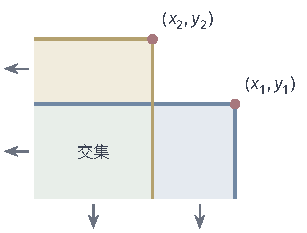
\includegraphics[width=52mm]{figures/07-probability/02-measure-theoretic-probability/tikz/pspace-pi-system/figure.pdf}
  \caption{左下象限构成$\pi$系统。以$(x_1,y_1)$为顶点的象限（浅蓝，蓝色边界）与以$(x_2,y_2)$为顶点的象限（浅黄，黄色边界）都向左、向下无限延伸，它们的交集（浅绿）仍是左下象限，顶点为$(\min\{x_1,x_2\},\min\{y_1,y_2\})$。}
  \label{fig:pspace-pi-system}
\end{BookInlineFigure}

\paragraph{分组保持独立}
第~\ref{chap:random-vectors}章还使用过一个事实：相互独立的变量分成互不相交的几组，各组的函数仍相互独立，例如$X_1+X_2$与$X_3^{2}$独立。现在可以对一般的可测函数证明它。

\begin{theorem}[分组定理]
\label{thm:pspace-grouping}
设$\{\mathcal{G}_i\}_{i\in I}$相互独立，$I_1,I_2,\dots$是$I$的两两不交的子集。令$\mathcal{H}_k$为由$\bigcup_{i\in I_k}\mathcal{G}_i$生成的$\sigma$代数。则$\mathcal{H}_1,\mathcal{H}_2,\dots$相互独立。
\end{theorem}

\begin{proof}
只需证明任意有限个$\mathcal{H}_1,\dots,\mathcal{H}_m$相互独立。令$\mathcal{C}_k$为形如$A_{i_1}\cap\cdots\cap A_{i_r}$的集合全体，其中$i_1,\dots,i_r$是$I_k$中有限个不同的指标，$A_{i_j}\in\mathcal{G}_{i_j}$。$\mathcal{C}_k$对交封闭，含有$\Omega$，且生成$\mathcal{H}_k$。

取$C_k\in\mathcal{C}_k$，$k=1,\dots,m$。不同组的指标互不相同，$C_1\cap\cdots\cap C_m$是来自有限个不同$\mathcal{G}_i$的事件之交。由$\{\mathcal{G}_i\}$的独立性，它的概率等于所有这些事件的概率之积；把乘积按组归并，又等于$\mathbb{P}(C_1)\cdots\mathbb{P}(C_m)$。由引理~\ref{lem:pspace-pi-independence}，$\mathcal{H}_1,\dots,\mathcal{H}_m$相互独立。
\end{proof}

若$X_1,X_2,X_3$相互独立，取$I_1=\{1,2\}$，$I_2=\{3\}$，则$\sigma(X_1,X_2)$与$\sigma(X_3)$独立。这里用到$\sigma(X_1,X_2)$就是由$\sigma(X_1)\cup\sigma(X_2)$生成的$\sigma$代数，因为$\mathcal{B}(\mathbb{R}^{2})$由矩形$B_1\times B_2$生成，而矩形的原像是
\[
  \{(X_1,X_2)\in B_1\times B_2\}=\{X_1\in B_1\}\cap\{X_2\in B_2\}.
\]
对任意Borel函数$g,h$，由上一节“函数只会减少信息”，$\sigma(g(X_1,X_2))\subseteq\sigma(X_1,X_2)$，$\sigma(h(X_3))\subseteq\sigma(X_3)$，所以$g(X_1,X_2)$与$h(X_3)$独立。$g$、$h$不必连续，也不必使原像是区间。

\paragraph{乘积测度给出独立对}
现在转向构造。给定两个概率空间$(E_1,\mathcal{E}_1,P_1)$与$(E_2,\mathcal{E}_2,P_2)$，要造一对独立的随机对象，分布分别是$P_1$和$P_2$。卷四的乘积测度正好做这件事：在$E_1\times E_2$上，乘积$\sigma$代数$\mathcal{E}_1\otimes\mathcal{E}_2$由可测矩形$A\times B$生成，其上存在唯一的概率测度$P_1\otimes P_2$，使
\begin{equation}
  (P_1\otimes P_2)(A\times B)=P_1(A)\,P_2(B),\qquad A\in\mathcal{E}_1,\ B\in\mathcal{E}_2 .
  \label{eq:pspace-product-measure}
\end{equation}
取$\Omega=E_1\times E_2$与$\mathbb{P}=P_1\otimes P_2$，令$X$、$Y$分别取$\omega=(\omega_1,\omega_2)$的第一、第二个坐标。这时
\[
  \{X\in A\}\cap\{Y\in B\}=A\times B,
\]
式~\eqref{eq:pspace-product-measure}说的正是$X$与$Y$独立，且$P_X=P_1$，$P_Y=P_2$。

反过来，独立性也可以完全用联合分布刻画。

\begin{theorem}[独立与乘积分布]
\label{thm:pspace-independence-product}
设$X,Y$分别取值于$(E_1,\mathcal{E}_1)$与$(E_2,\mathcal{E}_2)$。则$X$与$Y$独立，当且仅当
\begin{equation}
  P_{(X,Y)}=P_X\otimes P_Y .
  \label{eq:pspace-independence-product}
\end{equation}
\end{theorem}

\begin{proof}
若式~\eqref{eq:pspace-independence-product}成立，在矩形上取值就得到$\mathbb{P}(X\in A,Y\in B)=P_X(A)P_Y(B)$，即独立。反过来，若$X,Y$独立，则$P_{(X,Y)}$与$P_X\otimes P_Y$在全部可测矩形上取值相同。可测矩形对交封闭，因为
\[
  (A\times B)\cap(A'\times B')=(A\cap A')\times(B\cap B'),
\]
并且它们生成$\mathcal{E}_1\otimes\mathcal{E}_2$。两个概率测度在生成的$\pi$系统上一致，就处处一致。
\end{proof}

这个定理把“独立”从样本空间上的乘法公式，变成了取值空间上的一句话：联合分布是边缘分布的乘积。有密度时可以进一步写成密度的乘积。设$X,Y$分别有密度$f_X,f_Y$。由Tonelli定理，对矩形，
\[
  (P_X\otimes P_Y)(A\times B)=\int_Af_X\,\mathrm{d}x\int_Bf_Y\,\mathrm{d}y=\iint_{A\times B}f_X(x)f_Y(y)\,\mathrm{d}x\,\mathrm{d}y,
\]
再用$\pi$系统论证推广到一切Borel集，所以$f_X(x)f_Y(y)$是$P_X\otimes P_Y$的密度。于是：$X$与$Y$独立，当且仅当$f_X(x)f_Y(y)$是$(X,Y)$的一个联合密度。若$(X,Y)$另有联合密度$f$，同一个测度的两个密度只能在Lebesgue测度为零的集合上不同，可参考\BookChapterRef{chap:measure-densities}{卷四第8章“测度的密度”}；所以独立等价于$f=f_Xf_Y$几乎处处成立。这正是第~\ref{chap:random-vectors}章提到的情形：把联合密度在一条直线上改掉，它仍是联合密度，独立性不受影响。

\paragraph{一个独立对的计算}
设$X\sim\operatorname{Unif}(0,1)$，$Y\sim\operatorname{Exp}(1)$，二者独立，即$(X,Y)$的分布是$\operatorname{Unif}(0,1)\otimes\operatorname{Exp}(1)$。矩形事件直接相乘：
\[
  \mathbb{P}\bigl(X\leq\tfrac12,\ Y>1\bigr)=\tfrac12\cdot\mathrm{e}^{-1}\approx0.1839 .
\]
非矩形事件要对乘积测度积分。事件$\{Y>X\}$是正方形上方、对角线以上的区域。按$x$切片，每条竖直切片$\{y>x\}$在$Y$的分布下的质量是$\mathrm{e}^{-x}$，再对$x$在均匀分布下积分：
\[
  \mathbb{P}(Y>X)=\int_0^1\mathbb{P}(Y>x)\,\mathrm{d}x=\int_0^1\mathrm{e}^{-x}\,\mathrm{d}x=1-\mathrm{e}^{-1}\approx0.6321 .
\]
图~\ref{fig:pspace-product-measure}画出了这两个事件。第二步按切片积分的依据是Tonelli定理：被积函数是区域的示性函数，非负，可以先对$y$积分再对$x$积分。

\begin{BookInlineFigure}
  \centering
  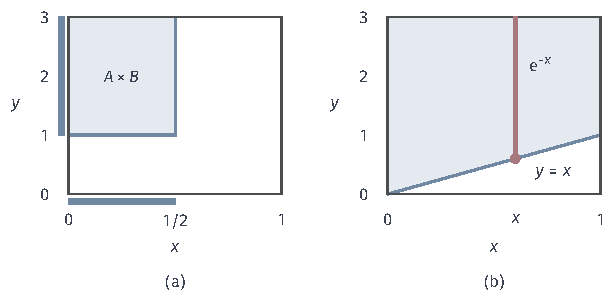
\includegraphics[width=104mm]{figures/07-probability/02-measure-theoretic-probability/tikz/pspace-product-measure/figure.pdf}
  \caption{$\operatorname{Unif}(0,1)\otimes\operatorname{Exp}(1)$上的两个事件，纵轴只画到$y=3$，区域向上延伸。(a)矩形$A\times B$，$A=[0,\tfrac12]$，$B=(1,\infty)$（坐标轴旁的粗线段），概率是两段边缘概率之积；(b)区域$\{y>x\}$，红色竖线是$x$处的切片，它在$Y$的分布下的质量是$\mathrm{e}^{-x}$。}
  \label{fig:pspace-product-measure}
\end{BookInlineFigure}

\paragraph{无穷多次抛硬币}
有限个独立对象由有限次乘积得到，可数个则需要无穷乘积。对实值的情形，木棍上的一个均匀点已经足够。仍取$\Omega=[0,1)$、长度测度，以及上一节的二进制数字$D_k(\omega)$。

\begin{theorem}[二进制数字独立]
\label{thm:pspace-binary-digits}
在$([0,1),\mathcal{B}([0,1)),\lambda)$上，$D_1,D_2,\dots$相互独立，且都服从$\operatorname{Bern}(1/2)$。
\end{theorem}

\begin{proof}
固定$n$与$d_1,\dots,d_n\in\{0,1\}$，令$a=\sum_{k=1}^{n}d_k2^{-k}$。按$D_k$的定义，$\omega$的前$n$位数字依次是$d_1,\dots,d_n$，当且仅当$\lfloor2^{n}\omega\rfloor=2^{n}a$，即
\[
  \{D_1=d_1,\dots,D_n=d_n\}=\bigl[a,\ a+2^{-n}\bigr).
\]
这个区间的长度是$2^{-n}$，所以
\[
  \mathbb{P}(D_1=d_1,\dots,D_n=d_n)=2^{-n}.
\]

对单个数字，把前$n$位中其余$n-1$位的所有取值加起来，得$\mathbb{P}(D_k=d)=2^{n-1}\cdot2^{-n}=1/2$。于是对前$n$个数字，联合概率等于各自概率之积。任意有限个数字都包含在某个前$n$个之中，对不出现的数字求和即可，所以任意有限子族满足乘法公式。数字只取两个值，$\sigma(D_k)$由$\{D_k=1\}$生成，乘法公式对$\sigma(D_k)$中的四个事件都成立。
\end{proof}

图~\ref{fig:pspace-binary-digits}画出了前三位数字。事件$\{D_1=1,D_3=0\}$由两段长$1/8$的区间组成，总长度$1/4=\frac12\cdot\frac12$，与乘法公式一致。

\begin{BookInlineFigure}
  \centering
  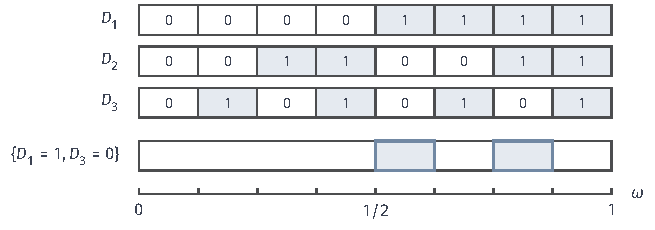
\includegraphics[width=111mm]{figures/07-probability/02-measure-theoretic-probability/tikz/pspace-binary-digits/figure.pdf}
  \caption{$[0,1)$上的二进制数字。前三行中，每个长$1/8$的格子里写着其中各点的第$k$位数字，浅蓝格子取值为$1$。最下一行是事件$\{D_1=1,D_3=0\}=[\tfrac12,\tfrac58)\cup[\tfrac34,\tfrac78)$，长度$\tfrac14$。}
  \label{fig:pspace-binary-digits}
\end{BookInlineFigure}

于是“无穷多次独立抛公平硬币”有了一个具体模型：样本点是木棍上的一个点，第$k$次的结果是它的第$k$位二进制数字。第~\ref{chap:random-variables}章的Cantor变量$\sum_k2D_k/3^{k}$就定义在这个空间上。“首次出现正面的次数”$T=\min\{k:D_k=1\}$也是如此，事件“永远不出现正面”是$\{T=\infty\}=\{0\}$：它非空，概率却为零，是第~\ref{sec:pspace-null-events}节所说的零概率而非不可能事件。

\paragraph{可数个独立的任意分布}
一个均匀点的数字可以拆成可数多组，每组再拼成一个均匀点。正整数$n$可以唯一地写成$n=2^{k-1}(2j-1)$，其中$k,j\geq1$：$k-1$是$n$中因子$2$的个数，$2j-1$是剩下的奇数部分。于是位置集合
\[
  I_k=\{2^{k-1}(2j-1):\ j=1,2,\dots\},\qquad k=1,2,\dots
\]
两两不交，并且覆盖全部正整数。令
\begin{equation}
  U_k=\sum_{j=1}^{\infty}D_{2^{k-1}(2j-1)}\,2^{-j},
  \label{eq:pspace-digit-split}
\end{equation}
即用第$k$组数字依次作为$U_k$的二进制数字（图~\ref{fig:pspace-digit-interleave}）。

\begin{BookInlineFigure}
  \centering
  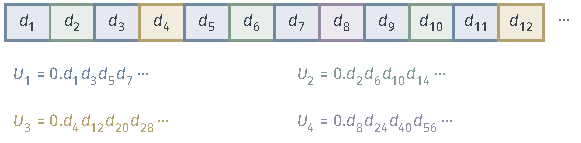
\includegraphics[width=98mm]{figures/07-probability/02-measure-theoretic-probability/tikz/pspace-digit-interleave/figure.pdf}
  \caption{把一个均匀点的二进制数字$d_1d_2d_3\cdots$分成互不相交的组。第$k$组由位置$2^{k-1}(2j-1)$组成，颜色相同的格子属于同一组：奇数位置给$U_1$（蓝），$2,6,10,\dots$给$U_2$（绿），$4,12,20,\dots$给$U_3$（黄），$8,24,\dots$给$U_4$（紫）。}
  \label{fig:pspace-digit-interleave}
\end{BookInlineFigure}

\begin{theorem}[独立序列的存在]
\label{thm:pspace-independent-sequence}
设$F_1,F_2,\dots$是一列满足定理~\ref{thm:pspace-cdf-measure}条件的函数。则在$([0,1),\mathcal{B}([0,1)),\lambda)$上存在相互独立的随机变量$X_1,X_2,\dots$，使$F_{X_k}=F_k$对每个$k$成立。
\end{theorem}

\begin{proof}
分三步。第一步说明$U_1,U_2,\dots$相互独立。$U_k$是第$k$组数字的部分和之极限，可测函数列的极限可测，所以$U_k$关于$\mathcal{H}_k=\sigma(D_n:n\in I_k)$可测，$\sigma(U_k)\subseteq\mathcal{H}_k$。各组位置互不相交，由定理~\ref{thm:pspace-binary-digits}与分组定理~\ref{thm:pspace-grouping}，$\mathcal{H}_1,\mathcal{H}_2,\dots$相互独立，于是$U_1,U_2,\dots$相互独立。

第二步说明每个$U_k$都是均匀分布。$U_k$的数字序列与$(D_1,D_2,\dots)$同样是独立的公平比特。对二进分点区间$J=[b2^{-m},(b+1)2^{-m})$，$U_k\in J$意味着$U_k$的前$m$位数字是$b$的二进制表示，除非$U_k$的数字从某一位起全为$1$。后一情形的概率为零：对固定的起始位置，“此后$r$位全为$1$”的概率是$2^{-r}$，令$r\to\infty$得零，再对可数个起始位置取并。于是
\[
  \mathbb{P}(U_k\in J)=2^{-m}=\lambda(J).
\]
二进分点区间与空集一起构成$\pi$系统，生成$\mathcal{B}([0,1))$，并且$\mathbb{P}(U_k\in[0,1))=1$，所以$U_k$的分布就是长度测度。

第三步作分位数变换。令$Q_k$为$F_k$的分位数函数，$U_k\in(0,1)$时令$X_k=Q_k(U_k)$，否则令$X_k=0$。$U_k$均匀分布，由定理~\ref{thm:pspace-quantile-transform}的证明，$F_{X_k}=F_k$。每个$X_k$是$U_k$的函数，由分组定理，$X_1,X_2,\dots$相互独立。
\end{proof}

第一部分及后续各章常说“取独立同分布的$X_1,X_2,\dots$”，这个定理保证了这样的序列确实存在，而且可以放在同一个概率空间上。取值于$\mathbb{R}^{d}$时，把每个$U_k$的数字再拆成$d$组，就得到$d$个独立坐标。对任意一列概率空间$(E_k,\mathcal{E}_k,P_k)$，可数乘积$\bigotimes_kP_k$在由“只限制有限个坐标”的柱集生成的$\sigma$代数上也存在且唯一，这一般性结论需要测度延拓的进一步论证，篇幅较长，读者可查阅~\scite{math-kallenberg2021probability}。本卷用到的独立序列都是实值或向量值的，上面的构造已经够用。

指标不可数时情况不同。连续时间的随机过程$\{X_t\}_{t\geq0}$也可以按有限个时刻的联合分布在乘积空间上构造，但“路径连续”这样的性质涉及不可数个时刻，不是由有限个坐标决定的事件，第~\ref{sec:pspace-null-events}节的尖峰例子已经显示了这类困难。处理它需要选择合适的版本并证明路径的正则性，可参考\BookChapterRef{chap:stochastic-processes-and-information}{卷九第2章“随机过程与随时间增长的信息”}。

\section{期望的积分表示}
\label{sec:pspace-expectation}

第~\ref{chap:random-variable-moments}章把期望定义为概率表上的加权和或密度的积分，等待时间$W$只能把两部分拆开计算，Cantor变量的期望则无从下手。另外几个结论也留了下来：两个任意随机变量之和的期望、求和与取极限的交换、用密度直接计算$\mathbb{E}[g(X)]$的公式。这些都归结为同一件事：期望是随机变量对概率测度的积分。

\paragraph{非负随机变量}
最简单的随机变量只取有限个值。设$A_1,\dots,A_m$是$\Omega$的一个划分，各块都是事件，$a_i\geq0$，
\[
  X=\sum_{i=1}^{m}a_i\mathbf{1}_{A_i}.
\]
这样的$X$称为简单随机变量，它在每一块上取常数值。它的期望只能是按块加权：
\[
  \mathbb{E}[X]=\sum_{i=1}^{m}a_i\,\mathbb{P}(A_i),
\]
这与第~\ref{chap:random-variable-moments}章对有限取值变量的定义一致。一般的非负随机变量用从下方逼近它的简单随机变量来定义，这就是卷四对非负可测函数的积分。

\begin{definition}[非负随机变量的期望]
\label{def:pspace-expectation-nonnegative}
设$X\geq0$是随机变量。称
\begin{equation}
  \mathbb{E}[X]=\int_{\Omega}X\,\mathrm{d}\mathbb{P}=\sup\bigl\{\mathbb{E}[\varphi]:\ \varphi\text{ 是简单随机变量},\ 0\leq\varphi\leq X\bigr\}
  \label{eq:pspace-expectation-nonnegative}
\end{equation}
为$X$的期望，它的值属于$[0,+\infty]$。
\end{definition}

上确界并不需要逐个比较。卷四给出了一列标准的逼近：
\begin{equation}
  \varphi_n=\min\Bigl\{n,\ \frac{\lfloor2^{n}X\rfloor}{2^{n}}\Bigr\},\qquad n=1,2,\dots .
  \label{eq:pspace-simple-approx}
\end{equation}
$\varphi_n$把$X$的取值向下取整到$2^{-n}$的整数倍，并在$n$处截断，它只取有限个值，且$\varphi_n\uparrow X$。由单调收敛定理，$\mathbb{E}[\varphi_n]\uparrow\mathbb{E}[X]$。

这个逼近与黎曼积分的思路不同。黎曼积分切分的是定义域，在$\Omega$上切小块；这里切分的是取值，把$X$的值分成宽$2^{-n}$的层，每层的值乘以落在这层的概率再相加。$\Omega$可以是任何集合，没有“小块”可言，按取值分层却总能进行，所需的只是每层$\{k2^{-n}\leq X<(k+1)2^{-n}\}$是事件，也就是$X$的可测性。

在木棍模型上看$X(\omega)=-\ln(1-\omega)$，它服从$\operatorname{Exp}(1)$。$n=1$时$\varphi_1$取三个值，
\[
  \varphi_1=\begin{cases}0,&X<\tfrac12,\\ \tfrac12,&\tfrac12\leq X<1,\\ 1,&X\geq1,\end{cases}
\]
各层的概率由指数分布的尾概率算出，于是
\[
  \mathbb{E}[\varphi_1]=\tfrac12\bigl(\mathrm{e}^{-1/2}-\mathrm{e}^{-1}\bigr)+1\cdot\mathrm{e}^{-1}\approx0.1193+0.3679=0.4872 .
\]
继续加细，前几项依次为
\[
  \mathbb{E}[\varphi_1]\approx0.4872,\quad \mathbb{E}[\varphi_2]\approx0.7611,\quad \mathbb{E}[\varphi_3]\approx0.8921,\quad \mathbb{E}[\varphi_4]\approx0.9513,
\]
它们递增地趋于$\mathbb{E}[X]=1$（图~\ref{fig:pspace-simple-approx}）。

\begin{BookInlineFigure}
  \centering
  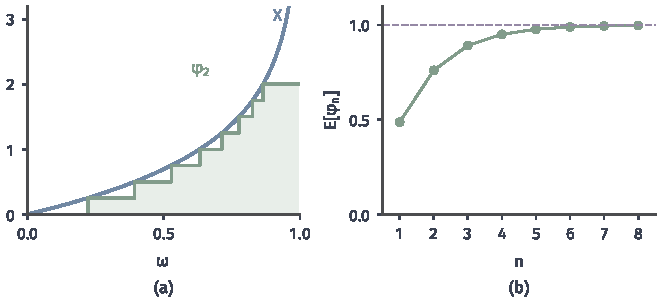
\includegraphics[width=112mm]{figures/07-probability/02-measure-theoretic-probability/matplotlib/pspace-simple-approx/figure.pdf}
  \caption{用简单随机变量逼近期望。(a)蓝线是$X(\omega)=-\ln(1-\omega)$，绿色阶梯是$\varphi_2$：取值向下取整到$1/4$的倍数并在$2$处截断，浅绿面积是$\mathbb{E}[\varphi_2]$；(b)绿点是$\mathbb{E}[\varphi_n]$，由式~\eqref{eq:pspace-simple-approx}按层精确算出，递增地趋于紫色虚线$\mathbb{E}[X]=1$。}
  \label{fig:pspace-simple-approx}
\end{BookInlineFigure}

\paragraph{有符号随机变量}
一般的随机变量拆成正部与负部，$X=X^{+}-X^{-}$，其中$X^{+}=\max\{X,0\}$，$X^{-}=\max\{-X,0\}$，两者都非负。

\begin{definition}[期望与可积]
\label{def:pspace-expectation}
设$X$是随机变量。若$\mathbb{E}[X^{+}]$与$\mathbb{E}[X^{-}]$至少有一个有限，定义
\begin{equation}
  \mathbb{E}[X]=\mathbb{E}[X^{+}]-\mathbb{E}[X^{-}].
  \label{eq:pspace-expectation}
\end{equation}
若$\mathbb{E}[X^{+}]$与$\mathbb{E}[X^{-}]$都有限，即$\mathbb{E}[\lvert X\rvert]<\infty$，称$X$可积。
\end{definition}

两部分都为无穷时期望没有定义，这正是第~\ref{chap:common-distributions}章对Cauchy分布的结论。可积的随机变量构成一个向量空间，期望是它上面的线性函数。

\begin{theorem}[期望的基本性质]
\label{thm:pspace-expectation-properties}
设$X,Y$是可积随机变量，$a,b\in\mathbb{R}$。
\begin{enumerate}
  \item 线性：$aX+bY$可积，且
  \begin{equation}
    \mathbb{E}[aX+bY]=a\,\mathbb{E}[X]+b\,\mathbb{E}[Y];
    \label{eq:pspace-linearity}
  \end{equation}
  \item 保序：若$X\leq Y$几乎必然成立，则$\mathbb{E}[X]\leq\mathbb{E}[Y]$；
  \item 绝对值估计：$\lvert\mathbb{E}[X]\rvert$不超过$\mathbb{E}[\lvert X\rvert]$；
  \item 若$X=Y$几乎必然成立，则$\mathbb{E}[X]=\mathbb{E}[Y]$；
  \item 若$X\geq0$且$\mathbb{E}[X]=0$，则$X=0$几乎必然成立。
\end{enumerate}
\end{theorem}

\begin{proof}
前四条是卷四积分的线性、单调性、绝对值估计以及“几乎处处相等的函数积分相同”，只是把测度取为$\mathbb{P}$。

第五条用一个分层估计。对正整数$n$，在$\{X>1/n\}$上$X>1/n$，在其余位置$X\geq0$，所以$\frac1n\mathbf{1}_{\{X>1/n\}}\leq X$。取期望，
\[
  \frac1n\,\mathbb{P}(X>1/n)\leq\mathbb{E}[X]=0 .
\]
于是每个$\{X>1/n\}$都是零概率事件。$\{X>0\}$是它们对$n$的并，由引理~\ref{lem:pspace-countable-null}，$\mathbb{P}(X>0)=0$。
\end{proof}

线性不要求知道$X$与$Y$的联合分布，也不要求它们独立：积分在每个样本点上逐点相加，$X(\omega)+Y(\omega)$在哪里取什么值，期望都按同一个$\mathbb{P}$加权。第~\ref{chap:random-variable-moments}章只对概率表证明了这一点，现在它对一切可积随机变量成立。

第五条补上第~\ref{chap:random-variable-moments}章关于方差的结论。设$X$平方可积且
\[
  \operatorname{Var}(X)=\mathbb{E}\bigl[(X-\mathbb{E}[X])^{2}\bigr]=0 .
\]
对非负变量$(X-\mathbb{E}[X])^{2}$用第五条，得$X=\mathbb{E}[X]$几乎必然成立。方差为零的随机变量几乎必然是常数，它在零概率事件上可以取别的值，但这不影响任何概率和期望。

\paragraph{期望与极限}
第~\ref{chap:random-variable-moments}章指出，对无穷多个随机变量之和逐项取期望，相当于交换求和与取极限的次序，需要额外的条件。卷四的两个收敛定理给出了这些条件，这里用概率的语言写出来。

\begin{theorem}[单调收敛与支配收敛]
\label{thm:pspace-convergence}
设$X_1,X_2,\dots$与$X$是随机变量，$X_n\to X$几乎必然成立。
\begin{enumerate}
  \item 若$0\leq X_1\leq X_2\leq\cdots$几乎必然成立，则
  \begin{equation}
    \lim_{n\to\infty}\mathbb{E}[X_n]=\mathbb{E}[X];
    \label{eq:pspace-monotone-convergence}
  \end{equation}
  \item 若存在可积的$Y$，使$\lvert X_n\rvert\leq Y$对每个$n$几乎必然成立，则$X$可积，且
  \begin{equation}
    \lim_{n\to\infty}\mathbb{E}[X_n]=\mathbb{E}[X].
    \label{eq:pspace-dominated-convergence}
  \end{equation}
\end{enumerate}
\end{theorem}

这是卷四单调收敛定理与支配收敛定理在概率测度下的特例。条件中的“几乎必然”无关紧要：由引理~\ref{lem:pspace-countable-null}，可数个几乎必然的条件同时在一个零概率事件之外成立，在那里把各变量改为$0$，期望都不变。

对非负随机变量列$Y_1,Y_2,\dots$，把单调收敛用于部分和$X_n=\sum_{k\leq n}Y_k$，得到
\begin{equation}
  \mathbb{E}\Bigl[\sum_{k=1}^{\infty}Y_k\Bigr]=\sum_{k=1}^{\infty}\mathbb{E}[Y_k],
  \label{eq:pspace-series-exchange}
\end{equation}
两边可以同为$+\infty$。若$Y_k$不一定非负，但$\sum_k\mathbb{E}[\lvert Y_k\rvert]<\infty$，则由式~\eqref{eq:pspace-series-exchange}，$Z=\sum_k\lvert Y_k\rvert$可积，它控制全部部分和，支配收敛给出同样的交换。一个常用的推论是：取值于$\{0,1,2,\dots\}$的随机变量$T$可以写成$T=\sum_{k\geq1}\mathbf{1}_{\{T\geq k\}}$，因为$T=m$时恰有$k=1,\dots,m$这$m$项为$1$。由式~\eqref{eq:pspace-series-exchange}，
\[
  \mathbb{E}[T]=\sum_{k=1}^{\infty}\mathbb{P}(T\geq k).
\]
对首次出现正面的次数$T$，$\mathbb{P}(T\geq k)$是前$k-1$次都是反面的概率$2^{-(k-1)}$，所以
\[
  \mathbb{E}[T]=\sum_{k=1}^{\infty}2^{-(k-1)}=2 .
\]

没有单调性或支配函数时，交换可能失败。在木棍模型上令$X_n=n\,\mathbf{1}_{(0,1/n)}$。对每个$\omega$，只要$n>1/\omega$就有$X_n(\omega)=0$，而$X_n(0)=0$，所以$X_n\to0$处处成立。可是
\[
  \mathbb{E}[X_n]=n\cdot\frac1n=1\quad\text{对每个}n,
\]
极限的期望是$0$，期望的极限是$1$。质量$1$被挤进越来越窄的区间，最后从每个固定位置“逃走”了；任何控制函数都要不小于$\sup_nX_n$，它在$(\frac1{k+1},\frac1k)$上至少为$k$，期望是发散的调和级数，不可积。

\paragraph{分布积分公式}
期望定义在$\Omega$上，计算却几乎总是在取值空间上进行。下面的公式说明这样做总是合法的，它是卷四推前积分恒等式在概率中的形式。

\begin{theorem}[分布积分公式]
\label{thm:pspace-law-integral}
设$X$是取值于$(E,\mathcal{E})$的随机对象，$g:E\to\mathbb{R}$可测。若$g\geq0$，或$g(X)$可积，则
\begin{equation}
  \mathbb{E}\bigl[g(X)\bigr]=\int_{E}g\,\mathrm{d}P_X .
  \label{eq:pspace-law-integral}
\end{equation}
\end{theorem}

\begin{proof}
沿着积分的定义逐步推广。若$g=\mathbf{1}_{B}$，$B\in\mathcal{E}$，则$g(X)=\mathbf{1}_{\{X\in B\}}$，两边都等于$\mathbb{P}(X\in B)=P_X(B)$。由线性，式~\eqref{eq:pspace-law-integral}对非负简单函数成立。

对非负可测的$g$，取非负简单函数$g_n\uparrow g$，则$g_n(X)$也是递增到$g(X)$的非负简单随机变量。两边分别用单调收敛定理，
\[
  \mathbb{E}\bigl[g(X)\bigr]=\lim_{n\to\infty}\mathbb{E}\bigl[g_n(X)\bigr]=\lim_{n\to\infty}\int_Eg_n\,\mathrm{d}P_X=\int_Eg\,\mathrm{d}P_X .
\]

对一般的$g$，把非负情形分别用于$g^{+}$和$g^{-}$。$g(X)$可积时两部分都有限，相减即得。
\end{proof}

公式的右边只含$P_X$，所以期望只依赖分布：同分布的随机变量期望相同，$X$定义在哪个概率空间上无关紧要。它还说明，计算$\mathbb{E}[g(X)]$不必先求$g(X)$的分布，直接在$X$的分布上积分$g$即可。第~\ref{chap:random-variable-moments}章的公式都是它的特例。

若$X$取可数个值，$P_X=\sum_xp_X(x)\delta_x$，其中$\delta_x$是$x$处的单点测度，对单点测度积分就是取值，于是
\[
  \mathbb{E}\bigl[g(X)\bigr]=\sum_xg(x)\,p_X(x).
\]
若$X$有密度$f_X$，$P_X$是以$f_X$为密度的加权测度，卷四测度的密度一章的加权积分规则给出
\[
  \mathbb{E}\bigl[g(X)\bigr]=\int_{\mathbb{R}}g(x)\,f_X(x)\,\mathrm{d}x .
\]
这对任何使右边有意义的Borel函数$g$都成立，包括示性函数和分段常数函数，不需要$g(X)$有密度。

等待时间的分布式~\eqref{eq:pspace-waiting-law}是单点测度与加权测度之和，积分也分成两项。取$g(x)=x$与$g(x)=x^{2}$，
\[
  \mathbb{E}[W]=0.3\cdot0+0.7\int_0^{\infty}t\,\mathrm{e}^{-t}\,\mathrm{d}t=0.7,\qquad \mathbb{E}[W^{2}]=0.7\int_0^{\infty}t^{2}\,\mathrm{e}^{-t}\,\mathrm{d}t=1.4 .
\]
于是
\[
  \operatorname{Var}(W)=1.4-0.7^{2}=0.91 .
\]
第~\ref{chap:random-variable-moments}章“跳跃部分求和、连续部分积分”的做法，现在是对两个测度之和积分的线性。

\paragraph{尾积分公式}
非负随机变量的期望还可以只用尾概率表示。第~\ref{chap:tail-probabilities}章在有密度时证明过这一点，那里交换积分次序的依据是Tonelli定理；现在对一般的非负随机变量写出完整的论证。

\begin{theorem}[尾积分公式]
\label{thm:pspace-tail-integral}
设$X\geq0$是随机变量，则
\begin{equation}
  \mathbb{E}[X]=\int_0^{\infty}\mathbb{P}(X>t)\,\mathrm{d}t,
  \label{eq:pspace-tail-integral}
\end{equation}
两边可以同为$+\infty$。
\end{theorem}

\begin{proof}
把每个样本点上的取值写成一段长度：
\[
  X(\omega)=\int_0^{\infty}\mathbf{1}_{\{t<X(\omega)\}}\,\mathrm{d}t .
\]
被积函数是集合$G=\{(\omega,t):0\leq t<X(\omega)\}$在$\Omega\times[0,\infty)$中的示性函数。$G$是乘积$\sigma$代数中的集合：若$t<X(\omega)$，可以取有理数$q$使$t<q<X(\omega)$，反之亦然，所以
\[
  G=\bigcup_{q\in\mathbb{Q},\,q>0}\bigl(\{X>q\}\times[0,q)\bigr),
\]
这是可数个可测矩形之并。

于是$\mathbf{1}_{G}$是$\mathbb{P}\otimes\lambda$下的非负可测函数，Tonelli定理允许交换积分次序：
\[
  \mathbb{E}[X]=\int_{\Omega}\int_0^{\infty}\mathbf{1}_{G}(\omega,t)\,\mathrm{d}t\,\mathbb{P}(\mathrm{d}\omega)=\int_0^{\infty}\int_{\Omega}\mathbf{1}_{G}(\omega,t)\,\mathbb{P}(\mathrm{d}\omega)\,\mathrm{d}t .
\]
内层积分是$\mathbb{P}(X>t)$，即得式~\eqref{eq:pspace-tail-integral}。
\end{proof}

这个证明是在计算同一块区域面积的两种切法。用分位数变换把$W$实现为$Q_W(U)$，区域$G$就是$Q_W$的图像下方（图~\ref{fig:pspace-tail-integral}(a)）。竖着切，每条竖线的长度是$Q_W(u)$，对$u$积分得$\mathbb{E}[W]$；横着切，高度$t$处的横线长度是$\mathbb{P}(W>t)$，对$t$积分得尾积分。对$W$，
\[
  \int_0^{\infty}\mathbb{P}(W>t)\,\mathrm{d}t=\int_0^{\infty}0.7\,\mathrm{e}^{-t}\,\mathrm{d}t=0.7,
\]
与分布积分公式的结果一致。在$t=0$处，$\mathbb{P}(W>0)=0.7$而不是$1$，因为$W=0$的那部分质量对任何$t\geq0$都不在$\{W>t\}$中，它对期望没有贡献。

\begin{BookInlineFigure}
  \centering
  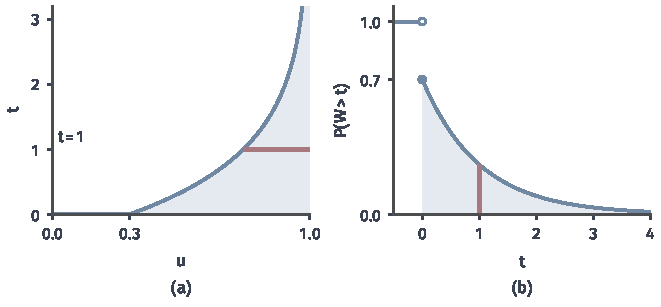
\includegraphics[width=112mm]{figures/07-probability/02-measure-theoretic-probability/matplotlib/pspace-tail-integral/figure.pdf}
  \caption{同一块面积的两种切法。(a)浅蓝区域在分位数函数$Q_W$的图像下方，红色横线是高度$t=1$处的切片，长度为$\mathbb{P}(W>1)=0.7\,\mathrm{e}^{-1}$；(b)蓝线是$\mathbb{P}(W>t)$，在$t=0$处从$1$降到$0.7$（实心点是函数值），红色竖线是同一个切片长度。两块浅蓝面积都等于$\mathbb{E}[W]=0.7$。}
  \label{fig:pspace-tail-integral}
\end{BookInlineFigure}

取值于非负整数时，$\mathbb{P}(T>t)$在每个区间$[k-1,k)$上等于$\mathbb{P}(T\geq k)$，式~\eqref{eq:pspace-tail-integral}就回到前面的级数公式$\mathbb{E}[T]=\sum_k\mathbb{P}(T\geq k)$。

\paragraph{独立对象的乘积期望}
第~\ref{chap:random-vectors}章对独立变量使用了$\mathbb{E}[XY]=\mathbb{E}[X]\,\mathbb{E}[Y]$，以及$\mathbb{E}[\phi(X,Y)]$的累次积分公式，在密度情形把它们当作计算规则。由乘积分布与分布积分公式，现在可以一般地证明。

\begin{theorem}[独立对象的期望]
\label{thm:pspace-independent-expectation}
设$X,Y$分别取值于$(E_1,\mathcal{E}_1)$与$(E_2,\mathcal{E}_2)$，相互独立，$\phi:E_1\times E_2\to\mathbb{R}$可测。若$\phi\geq0$，或$\phi(X,Y)$可积，则
\begin{equation}
  \mathbb{E}\bigl[\phi(X,Y)\bigr]=\int_{E_1}\Bigl(\int_{E_2}\phi(x,y)\,P_Y(\mathrm{d}y)\Bigr)P_X(\mathrm{d}x).
  \label{eq:pspace-independent-iterated}
\end{equation}
特别地，若实值随机变量$X,Y$独立且都可积，则$XY$可积，并且
\begin{equation}
  \mathbb{E}[XY]=\mathbb{E}[X]\,\mathbb{E}[Y].
  \label{eq:pspace-independent-product}
\end{equation}
\end{theorem}

\begin{proof}
由分布积分公式，$\mathbb{E}[\phi(X,Y)]$等于$\phi$对$P_{(X,Y)}$的积分。由定理~\ref{thm:pspace-independence-product}，$P_{(X,Y)}=P_X\otimes P_Y$。$\phi\geq0$时用Tonelli定理化为累次积分，即得式~\eqref{eq:pspace-independent-iterated}；$\phi(X,Y)$可积时用Fubini定理。

对乘积，先取$\phi(x,y)=\lvert x\rvert\lvert y\rvert\geq0$，内层积分是$\lvert x\rvert\,\mathbb{E}[\lvert Y\rvert]$，于是
\[
  \mathbb{E}\bigl[\lvert XY\rvert\bigr]=\mathbb{E}\bigl[\lvert X\rvert\bigr]\,\mathbb{E}\bigl[\lvert Y\rvert\bigr]<\infty,
\]
$XY$可积。再取$\phi(x,y)=xy$，用Fubini定理，内层积分是$x\,\mathbb{E}[Y]$，外层再积分得到式~\eqref{eq:pspace-independent-product}。
\end{proof}

用第~\ref{sec:pspace-independence}节的独立对$X\sim\operatorname{Unif}(0,1)$、$Y\sim\operatorname{Exp}(1)$算两个例子。由式~\eqref{eq:pspace-independent-product}，
\[
  \mathbb{E}[XY]=\tfrac12\cdot1=\tfrac12 .
\]
对$\phi(x,y)=\mathrm{e}^{-xy}$，它不是乘积形式，只能用累次积分。先对$y$积分，
\[
  \int_0^{\infty}\mathrm{e}^{-xy}\,\mathrm{e}^{-y}\,\mathrm{d}y=\frac{1}{1+x},
\]
再对$x$在$[0,1]$上积分，
\[
  \mathbb{E}\bigl[\mathrm{e}^{-XY}\bigr]=\int_0^1\frac{\mathrm{d}x}{1+x}=\ln2\approx0.6931 .
\]
式~\eqref{eq:pspace-independent-product}只是独立的一个推论，反过来不成立：第~\ref{chap:random-vectors}章已经看到，$\mathbb{E}[XY]=\mathbb{E}[X]\,\mathbb{E}[Y]$只说明不相关，不能推出独立。

\paragraph{Cantor变量的均值与方差}
最后回到章首的Cantor变量$X$，它等于$\sum_{k\geq1}2D_k/3^{k}$，其中$D_k$是第~\ref{sec:pspace-independence}节的独立公平比特。它既没有概率表也没有密度，可是$X$是非负随机变量，期望有定义。由式~\eqref{eq:pspace-series-exchange}，
\[
  \mathbb{E}[X]=\sum_{k=1}^{\infty}\frac{2\,\mathbb{E}[D_k]}{3^{k}}=\sum_{k=1}^{\infty}\frac{1}{3^{k}}=\frac12 .
\]
这与对称性一致：把每个$D_k$换成$1-D_k$，$X$变成$1-X$，而独立公平比特在这一替换下联合分布不变，所以$X\overset{\mathrm{d}}{=}1-X$。

方差要用支配收敛。令$\varepsilon_k=2D_k-1$，它等概率地取$\pm1$，各$\varepsilon_k$相互独立。记部分和
\[
  S_n=\sum_{k=1}^{n}\frac{\varepsilon_k}{3^{k}},\qquad \lvert S_n\rvert\leq\sum_{k=1}^{\infty}\frac{1}{3^{k}}=\frac12,
\]
它处处收敛到$X-\frac12$。展开平方，
\[
  \mathbb{E}[S_n^{2}]=\sum_{k=1}^{n}\frac{\mathbb{E}[\varepsilon_k^{2}]}{9^{k}}+\sum_{j\neq k}\frac{\mathbb{E}[\varepsilon_j\varepsilon_k]}{3^{j+k}}=\sum_{k=1}^{n}\frac{1}{9^{k}},
\]
其中$\varepsilon_k^{2}=1$，而$j\neq k$时$\varepsilon_j$与$\varepsilon_k$独立、均值为零，由式~\eqref{eq:pspace-independent-product}，交叉项的期望为零。

$S_n^{2}\to(X-\frac12)^{2}$处处成立，且$S_n^{2}\leq\frac14$，常数$\frac14$可积。由支配收敛定理，
\[
  \operatorname{Var}(X)=\lim_{n\to\infty}\mathbb{E}[S_n^{2}]=\sum_{k=1}^{\infty}\frac{1}{9^{k}}=\frac{1/9}{1-1/9}=\frac18 .
\]
标准差$\sqrt{1/8}\approx0.354$。图~\ref{fig:pspace-cantor-mean}是$20000$个模拟样本的直方图，样本均值约$0.498$，样本方差约$0.1250$。质量全部在Cantor集附近的若干小段上，均值$1/2$本身却落在中间被挖去的空隙里，没有任何样本能取到它；这再次说明期望是质量的重心，不必是可能的取值。

\begin{BookInlineFigure}
  \centering
  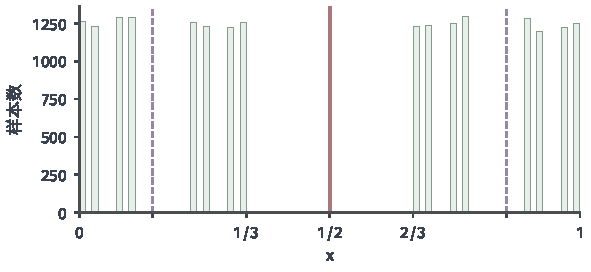
\includegraphics[width=100mm]{figures/07-probability/02-measure-theoretic-probability/matplotlib/pspace-cantor-mean/figure.pdf}
  \caption{Cantor变量的$20000$个模拟样本（每个样本保留$30$位三进制数字，种子$2026$），浅绿柱为$81$等分的直方图。红线是期望$1/2$，紫色虚线是$\frac12\pm\sqrt{1/8}$。样本都落在第二层保留的四段区间内，期望处于中间的空隙中。}
  \label{fig:pspace-cantor-mean}
\end{BookInlineFigure}

\paragraph{第一部分公式的来源}
表~\ref{tab:pspace-formula-sources}把第一部分的期望计算与它们在一般框架中的依据对应起来。每一行左边的公式，在第一部分只对概率表或密度验证过；右边的依据对任意分布都成立。

\begin{BookInlineTable}
  \centering
  \caption{第一部分的期望计算及其一般依据}
  \label{tab:pspace-formula-sources}
  \begin{tabular}{ll}
    \toprule
    第一部分的计算 & 一般框架中的依据 \\
    \midrule
    概率表求和$\sum_xg(x)p_X(x)$ & 分布积分公式，单点测度之和 \\
    密度积分$\int g(x)f_X(x)\,\mathrm{d}x$ & 分布积分公式，加权测度 \\
    混合分布分两部分计算 & 测度之和的积分 \\
    $\mathbb{E}[X+Y]=\mathbb{E}[X]+\mathbb{E}[Y]$ & 积分的线性 \\
    级数与期望交换 & 单调收敛、支配收敛 \\
    尾积分公式 & Tonelli定理 \\
    独立时$\mathbb{E}[XY]=\mathbb{E}[X]\,\mathbb{E}[Y]$ & 乘积分布与Fubini定理 \\
    \bottomrule
  \end{tabular}
\end{BookInlineTable}

\section{本章小结}
\label{sec:pspace-summary}

本章把第一部分分散的模型放进同一个框架。一个概率模型由三部分组成：样本空间$\Omega$列出可能的结果，事件族$\mathcal{F}$规定可以问概率的结果集合，概率测度$\mathbb{P}$给每个事件指定概率。事件族之所以要单独指定，是因为连续位置上无法给全部子集一致地赋予长度，也因为同一组结果在不同的观察者那里能回答的问题不同。它对补集和可数并封闭，因而是$\sigma$代数；在有限样本空间上，它就是一个划分及其各种并。

概率是总质量为一的测度。可数可加性推出概率沿单调事件列连续，由此得到分布函数的右连续性、两端极限和跳跃等于单点概率；分布函数又唯一确定实轴上的概率测度，任何满足三条性质的函数都对应一个分布，Cantor分布也在其中。单点概率为零与总概率为一并不矛盾，因为可加性只对可数个事件成立。零概率事件可以发生，几乎必然的陈述可以合并可数次，但不能合并不可数次；完备化把零概率事件的子集补为事件，使零概率修改不破坏可测性，却不改变任何原有概率，也不能使零概率条件变得可以相除。

随机对象是可测映射，可测性保证由观测引出的“取值落在某集合中”都是事件。实值、向量、矩阵和有限随机图都是它的特例，可测函数的复合仍是随机对象。观测生成的$\sigma$代数记录了它能区分的事件，对观测再作变换只会减少信息。随机对象的分布是概率在它下面的推前，变换后的分布由原像规则直接算出；分位数变换说明任何一维分布都可以由一个均匀随机点实现。处处相等、几乎必然相等与同分布依次减弱，边缘分布不能确定两个变量怎样配对，差与和的分布需要联合分布。

独立是信息族之间的乘法公式。它只需在对交封闭的生成族上检验，所以联合分布函数分解为乘积就足以推出独立；独立变量分组后的函数仍然独立。乘积测度造出了具有给定分布的独立对，独立等价于联合分布是边缘分布的乘积；木棍上一个均匀点的二进制数字是一列独立的公平比特，把这些数字拆组再作分位数变换，就得到具有任意分布的独立序列。

期望是随机变量对概率测度的积分：非负变量先用按取值分层的简单变量逼近，有符号变量再拆成正部与负部。线性、保序、单调收敛与支配收敛、分布积分公式、尾积分公式和独立乘积的期望，都是卷四积分理论的概率形式；第一部分的求和、密度积分和混合计算是它们的特例，等待时间的期望$0.7$与Cantor变量的方差$1/8$由此算出。

本章没有处理的是给定信息之后的平均。$\sigma(X)$描述了观测$X$提供的信息，下一章研究固定这部分信息、在每组已知结果内求平均得到的随机变量，即条件期望，并说明在观测值本身概率为零时怎样保留“组内平均”的含义。


\chapter{条件期望}
\label{chap:conditional-expectation}

第~\ref{chap:random-vectors}章已经会算给定一个读数后的平均。两台传感器的概率表中，第一台读$0$时，第二台的平均读数是第一行的加权平均$1/3$；三角形上的均匀分布中，给定$X=x$时$Y$的平均是$x/2$。前者把概率表的一行重新归一，后者把联合密度的一条切片除以它的总积分。

换一个问题，这两种办法都会失效。设$X$在$(-1,1)$上均匀分布，我们只知道它的绝对值$\lvert X\rvert$，想求$X$的正部$X^{+}=\max(X,0)$的平均。知道$\lvert X\rvert=0.6$，就知道$X$是$0.6$或$-0.6$，两者对称，$X^{+}$的平均应当是$0.3$。可是$\{\lvert X\rvert=0.6\}$的概率为零，不能拿它去除；$(X,\lvert X\rvert)$的全部质量落在平面上的两条线段上，也没有联合密度可以切片。直觉给出的答案很清楚，现有的公式却算不出来。

给定的信息也不一定来自某个数值读数。把$[0,1)$等分成四段，只告诉我们样本点落在哪一段，这同样是一份信息；再细分成八段，信息就更多。我们需要一种不依赖概率表或密度、对任意形式的已知信息都能用的条件平均。

本章的办法是不再去除单个条件的概率，而是要求条件平均在每个“已知能否判断其发生”的事件上，保留原变量的累计期望。

第一节从有限分组的组内平均出发，提炼出这一积分刻画，用Radon--Nikodym定理证明它总有解并且几乎必然唯一，再说明给定随机变量时它为何是该变量的函数。第二节在固定的信息下建立线性、保序与提取已知量等运算规则，并讨论独立的信息。第三节研究信息改变时条件平均怎样叠加，得到全期望公式和塔式法则。第四节用凸性比较“先平均再变换”与“先变换再平均”，第五节在平方可积的情形把条件期望解释为最佳预测与正交投影，并把总方差拆成组内与组间两部分。

全章沿用第~\ref{chap:random-vectors}章的两台传感器的概率表作为有限的贯穿例子，用$[0,1)$上$X(\omega)=\omega^{2}$的逐次等分作为连续样本空间上的例子，并用上面的“只知绝对值”作为分组概率为零的例子。比条件平均更完整的对象，即给定信息后的整个条件分布，在第~\ref{chap:conditional-distributions}章建立。

\section{条件期望的定义}
\label{sec:cexp-definition}

第~\ref{chap:random-vectors}章的条件均值都靠除法得到：组内的累计期望除以这一组的概率。只要组的概率为正，这个除法就有意义；一旦条件事件的概率为零，或者根本没有概率表和密度，它就失效。这一节先把有限分组的组内平均重新写成一个随机变量，找出它满足的两条性质；再把这两条性质当作定义，使它在分组概率为零时依然有意义；然后证明这样的随机变量存在而且几乎必然唯一；最后回到给定一个观测的情形，说明条件平均为什么是观测值的函数。

\subsection{有限分组中的条件平均}
\label{sec:cexp-finite-partition}

\paragraph{把组内平均写成随机变量}
回到两台传感器。第一台的档位为$X$，第二台为$Y$，联合概率表见图~\ref{fig:cexp-sensor-rows}(a)。把表中九个格子看作样本空间$\Omega$的九个样本点，每个格子的概率就是表中的数，其中$(0,2)$与$(2,0)$两格的概率为零。$X$与$Y$是这九个点上的函数：格子$(x,y)$上$X=x$，$Y=y$。

\begin{BookInlineFigure}
  \centering
  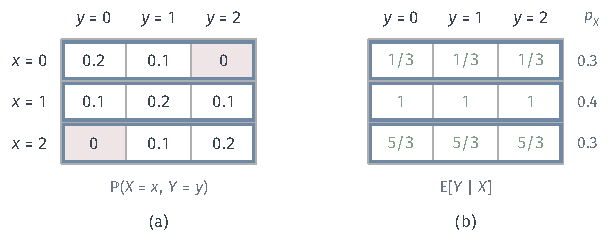
\includegraphics[width=104mm]{figures/07-probability/02-measure-theoretic-probability/tikz/cexp-sensor-rows/figure.pdf}
  \caption{传感器表上的组内平均。(a)九个格子组成样本空间，格中是概率，浅红格的概率为零；蓝框是按$X$的取值分成的三组。(b)随机变量$\mathbb{E}[Y\mid X]$：同一行的每个格子都取这一行$Y$的平均$1/3$、$1$、$5/3$，右侧是各行的概率$p_X$。}
  \label{fig:cexp-sensor-rows}
\end{BookInlineFigure}

知道$X$的值，相当于知道样本点落在哪一行。第~\ref{chap:random-vectors}章算出三行的条件均值$m(0)=1/3$、$m(1)=1$、$m(2)=5/3$。把这三个数填回格子，每一行的所有格子都填该行的均值，就得到图~\ref{fig:cexp-sensor-rows}(b)：一个定义在$\Omega$上的新函数，也就是随机变量$m(X)$。它在样本点$\omega$处的值，是“与$\omega$同组的所有样本点上$Y$的平均”。这个随机变量记作$\mathbb{E}[Y\mid X]$。

这样看，条件平均有两种身份。$m(x)$是一个数，回答“已知$X=x$时$Y$平均是多少”；$\mathbb{E}[Y\mid X]$是一个随机变量，回答“在还不知道结果时，按将来会得到的信息所作的平均是什么”。后者把三个问题的答案一次装进一个对象，本章研究的正是这个对象。

\paragraph{一般的有限分组}
分组不必按某个变量的取值进行。设事件$A_1,\dots,A_k$两两不交，并起来是$\Omega$，称为$\Omega$的一个有限划分。知道“样本点落在哪一组”，就能判断由若干组并成的任何事件是否发生；把这些并集合起来（包括空集），得到
\[
 \mathcal{G}=\Bigl\{\textstyle\bigcup_{i\in S}A_i:\ S\subseteq\{1,\dots,k\}\Bigr\},
\]
它恰好有$2^{k}$个事件。$\mathcal{G}$对补和并封闭，是一个$\sigma$代数，并且是包含$A_1,\dots,A_k$的最小$\sigma$代数。第~\ref{chap:probability-spaces}章用$\sigma$代数表示观测所能区分的信息，$\mathcal{G}$就是“知道所在组”这份信息。按$X$分行时，$\mathcal{G}=\sigma(X)$。

对可积的随机变量$X$，在每个概率为正的组内求平均，再把平均值赋给该组的所有样本点，就得到有限划分下的条件期望：
\begin{equation}
 \mathbb{E}[X\mid\mathcal{G}]=\sum_{i=1}^{k}c_i\mathbf{1}_{A_i},\qquad
 c_i=\frac{\mathbb{E}[X\mathbf{1}_{A_i}]}{\mathbb{P}(A_i)}\quad\text{当}\ \mathbb{P}(A_i)>0 .
 \label{eq:cexp-partition}
\end{equation}
$c_i$正是第~\ref{chap:classical-probability}章“缩小样本范围再重新归一”的平均：把$X$限制在$A_i$上求期望，再除以$A_i$的概率。$\mathbb{P}(A_i)=0$的组没有可以除的数，$c_i$任取一个常数。

\paragraph{概率为零的组}
按读数之差$D=X-Y$分组，就会遇到这种组。$D$取$-2,-1,0,1,2$五个值，对应传感器表的五条对角线，见图~\ref{fig:cexp-difference-groups}(a)。$D=2$与$D=-2$各只含一个概率为零的格子：两台读数从不相差两档。

\begin{BookInlineFigure}
  \centering
  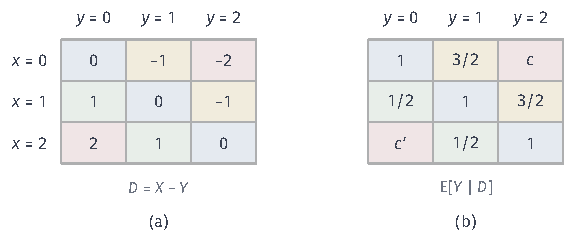
\includegraphics[width=96mm]{figures/07-probability/02-measure-theoretic-probability/tikz/cexp-difference-groups/figure.pdf}
  \caption{按读数之差$D=X-Y$分组。(a)每个格子所属的组，同色格子同组；浅红的两组$D=\pm2$概率为零。(b)$\mathbb{E}[Y\mid D]$在三组正概率组上分别取$1$、$1/2$、$3/2$，在两个零概率组上取任意常数$c$、$c'$。}
  \label{fig:cexp-difference-groups}
\end{BookInlineFigure}

由式~\eqref{eq:cexp-partition}逐组计算。$D=0$的三个格子概率都是$0.2$，$Y$分别取$0,1,2$；$D=1$的两个格子是$(1,0)$与$(2,1)$，概率都是$0.1$；$D=-1$的两个格子是$(0,1)$与$(1,2)$。于是
\[
 \begin{gathered}
 c_{D=0}=\frac{0.2\cdot(0+1+2)}{0.6}=1,\\
 c_{D=1}=\frac{0.1\cdot(0+1)}{0.2}=\frac12,\qquad
 c_{D=-1}=\frac{0.1\cdot(1+2)}{0.2}=\frac32 .
 \end{gathered}
\]
两台读数一致时，第二台的平均档位是$1$；第一台比第二台高一档时，第二台偏低，平均$1/2$；反过来平均$3/2$。$D=\pm2$两组上的值没有可算的依据，图~\ref{fig:cexp-difference-groups}(b)记作$c$与$c'$。

\paragraph{两条性质}
式~\eqref{eq:cexp-partition}得到的随机变量$Z=\mathbb{E}[X\mid\mathcal{G}]$有两条性质，它们后面会变成定义。

第一条，$Z$在每一组内取常数，所以只用到“所在组”这份信息。用$\sigma$代数的语言说：对任何实数集合$B$，$\{Z\in B\}$是若干整组的并，属于$\mathcal{G}$，即$Z$是$\mathcal{G}$可测的。反过来，一个$\mathcal{G}$可测的函数也必定在每组内取常数，因为单点集的原像$\{Z=z\}$只能是整组的并。

第二条，$Z$在每个已知事件上保留$X$的累计期望：
\[
 \mathbb{E}[Z\mathbf{1}_{A}]=\mathbb{E}[X\mathbf{1}_{A}],\qquad A\in\mathcal{G}.
\]
证明只需逐组核对。$A$是若干组$A_i$的并，两边都按组拆成和。对$\mathbb{P}(A_i)>0$的组，由$c_i$的定义，
\[
 \mathbb{E}[Z\mathbf{1}_{A_i}]=c_i\,\mathbb{P}(A_i)=\mathbb{E}[X\mathbf{1}_{A_i}] .
\]
对$\mathbb{P}(A_i)=0$的组，$\mathbf{1}_{A_i}$只在零概率集上非零，两边都是$0$，与$c_i$怎样选无关。把各组相加，就得到上式。

用$D$分组核对一次。取$A=\{D=0\}\cup\{D=1\}$。$Y$在这五个格子上的累计期望为
\[
 \mathbb{E}[Y\mathbf{1}_{A}]=0.2\cdot(0+1+2)+0.1\cdot(0+1)=0.7 ,
\]
而$Z=\mathbb{E}[Y\mid D]$在其中三格取$1$、两格取$1/2$，
\[
 \mathbb{E}[Z\mathbf{1}_{A}]=1\cdot0.6+\tfrac12\cdot0.2=0.7 .
\]
若把$A$换成含有零概率组的事件，例如再并上$\{D=2\}$，两边都不变，$c'$的取值不起作用。

\paragraph{连续样本空间上的有限分组}
样本空间本身不必有限。取$\Omega=[0,1)$，概率是区间长度，令$X(\omega)=\omega^{2}$。把$[0,1)$等分成$2^{n}$段，记这些区间生成的$\sigma$代数为$\mathcal{G}_n$，它表示“只知道$\omega$落在哪一段”。每段的概率为$2^{-n}>0$，式~\eqref{eq:cexp-partition}直接适用。区间$[a,b)$上的平均为
\[
 \frac{1}{b-a}\int_{a}^{b}\omega^{2}\,\mathrm{d}\omega=\frac{a^{2}+ab+b^{2}}{3}.
\]

取$n=2$，四段是$[0,\tfrac14)$、$[\tfrac14,\tfrac12)$、$[\tfrac12,\tfrac34)$、$[\tfrac34,1)$，代入上式，例如第二段为$(\tfrac1{16}+\tfrac18+\tfrac14)/3=\tfrac{7}{48}$，四段依次得到
\[
 \tfrac{1}{48},\qquad \tfrac{7}{48},\qquad \tfrac{19}{48},\qquad \tfrac{37}{48}.
\]
$\mathbb{E}[X\mid\mathcal{G}_2]$是取这四个值的阶梯函数，见图~\ref{fig:cexp-dyadic-average}(a)。在每一段内，阶梯下方的面积与抛物线下方的面积相等，浅蓝的两块“多出”与“缺少”的面积互相抵消，这正是第二条性质在单个组上的样子。分得越细，阶梯越贴近$X$，见图~\ref{fig:cexp-dyadic-average}(b)：信息越多，条件平均保留的$X$的细节越多。

\begin{BookInlineFigure}
  \centering
  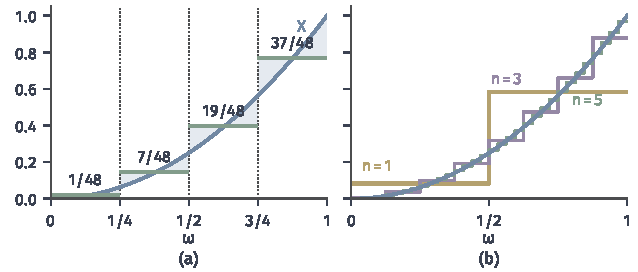
\includegraphics[width=108mm]{figures/07-probability/02-measure-theoretic-probability/matplotlib/cexp-dyadic-average/figure.pdf}
  \caption{$\Omega=[0,1)$上的均匀概率，$X(\omega)=\omega^{2}$（蓝）。(a)$\mathcal{G}_2$由四个等长区间生成，$\mathbb{E}[X\mid\mathcal{G}_2]$（绿）在各段取段内平均；每段内抛物线与阶梯之间的两块浅蓝面积相等。(b)$n=1$（黄）、$n=3$（紫）、$n=5$（绿）时的$\mathbb{E}[X\mid\mathcal{G}_n]$。}
  \label{fig:cexp-dyadic-average}
\end{BookInlineFigure}

\subsection{积分刻画}
\label{sec:cexp-integral}

\paragraph{分组的概率为零时}
回到章首的例子。取$\Omega=(-1,1)$，概率为长度的一半，令$X(\omega)=\omega$，于是$X\sim\operatorname{Unif}(-1,1)$；观测是$Y=\lvert X\rvert$。知道$Y$，就知道样本点在$\{\omega,-\omega\}$这一对之中，所以$\sigma(Y)$把$\Omega$分成不可数多个两点组，每组概率为零。式~\eqref{eq:cexp-partition}一个组也用不上。

直觉的答案是：同组两点概率对称，组内平均就是两点上函数值的算术平均。对正部$X^{+}$，在$\{\omega,-\omega\}$上的两个值是$\lvert\omega\rvert$与$0$，平均为$\lvert\omega\rvert/2$，所以候选答案是
\[
 Z=\frac{Y}{2}=\frac{\lvert X\rvert}{2}.
\]
图~\ref{fig:cexp-folding}(a)画出了它：红色虚线连接$\omega=\pm0.6$处的$X^{+}$，两端的平均$0.3$被赋给这两个点。

\begin{BookInlineFigure}
  \centering
  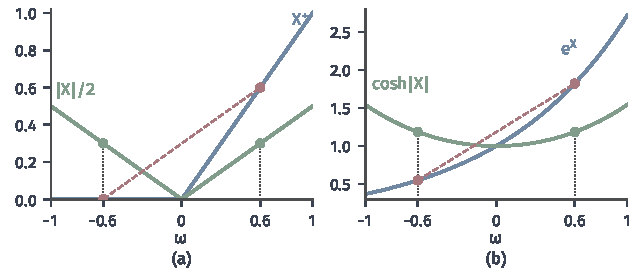
\includegraphics[width=108mm]{figures/07-probability/02-measure-theoretic-probability/matplotlib/cexp-folding/figure.pdf}
  \caption{只知道绝对值时的条件平均，$\Omega=(-1,1)$，$X(\omega)=\omega$均匀分布。(a)$X^{+}$（蓝）与候选的$\mathbb{E}[X^{+}\mid\lvert X\rvert]=\lvert X\rvert/2$（绿）；红点是同组的$\omega=\pm0.6$，两个函数值的平均$0.3$赋给这两点（绿点）。(b)同样地，$\mathrm{e}^{X}$（蓝）的组内平均是$\cosh\lvert X\rvert$（绿）。}
  \label{fig:cexp-folding}
\end{BookInlineFigure}

这个候选不能靠除法检验，但可以用上一小节的第二条性质检验。$\sigma(Y)$中的事件都形如$\{Y\in B\}$，$B\subseteq[0,1)$。$X$的密度在$(-1,1)$上是$\tfrac12$，于是
\[
 \mathbb{E}\bigl[X^{+}\mathbf{1}_{\{Y\in B\}}\bigr]
 =\int_{-1}^{1}\max(x,0)\,\mathbf{1}_{B}(\lvert x\rvert)\,\frac{\mathrm{d}x}{2}
 =\frac12\int_{0}^{1}x\,\mathbf{1}_{B}(x)\,\mathrm{d}x .
\]
另一边，$\lvert x\rvert/2$在$\pm x$处取同一个值，把$(-1,0)$与$(0,1)$两半合并，
\[
 \mathbb{E}\Bigl[\frac{Y}{2}\mathbf{1}_{\{Y\in B\}}\Bigr]
 =\int_{-1}^{1}\frac{\lvert x\rvert}{2}\,\mathbf{1}_{B}(\lvert x\rvert)\,\frac{\mathrm{d}x}{2}
 =\frac12\int_{0}^{1}x\,\mathbf{1}_{B}(x)\,\mathrm{d}x .
\]
两边对每个$B$都相等。候选答案在每个已知事件上保留了$X^{+}$的累计期望，尽管没有一个组可以单独拿来做除法。

\paragraph{定义}
这个例子说明，“在已知事件上保留累计期望”不需要除以组的概率，可以直接拿来作定义；再配上“只用已知信息”这一条，就把有限划分的情形推广到任意的信息。下面固定概率空间$(\Omega,\mathcal{F},\mathbb{P})$和一个$\sigma$代数$\mathcal{G}\subseteq\mathcal{F}$，$\mathcal{G}$表示已知的信息。

\begin{definition}[条件期望]
\label{def:cexp-conditional-expectation}
设$X$是可积的实随机变量，$\mathcal{G}\subseteq\mathcal{F}$是$\sigma$代数。若随机变量$Z$满足：
\begin{enumerate}
 \item $Z$是$\mathcal{G}$可测的；
 \item $Z$可积；
 \item 对每个$A\in\mathcal{G}$，
 \begin{equation}
  \mathbb{E}[Z\mathbf{1}_{A}]=\mathbb{E}[X\mathbf{1}_{A}],
  \label{eq:cexp-defining}
 \end{equation}
\end{enumerate}
则称$Z$为$X$给定$\mathcal{G}$的\term{条件期望}（conditional expectation），记作$\mathbb{E}[X\mid\mathcal{G}]$。满足要求的$Z$可能不止一个，其中每一个都称为\term{条件期望的版本}（version of a conditional expectation）。
\end{definition}

三条要求各有分工。$\mathcal{G}$可测限制了$Z$能用的信息：对每个Borel集$B$，“$Z\in B$是否发生”都必须能由已知事件判断，有限划分时这就是“组内取常数”。可积保证式~\eqref{eq:cexp-defining}左边有意义。式~\eqref{eq:cexp-defining}本身保证每个已知群体的平均不变：当$\mathbb{P}(A)>0$时两边同除以$\mathbb{P}(A)$，它说$Z$与$X$在$A$上的平均相同。

两种极端情形有助于看清定义。若$\mathcal{G}=\{\emptyset,\Omega\}$，什么也不知道，$\mathcal{G}$可测的随机变量只有常数，式~\eqref{eq:cexp-defining}对$A=\Omega$给出常数等于$\mathbb{E}[X]$，所以$\mathbb{E}[X\mid\mathcal{G}]=\mathbb{E}[X]$。若$X$本身是$\mathcal{G}$可测的，什么都已知道，$Z=X$满足全部三条，$\mathbb{E}[X\mid\mathcal{G}]=X$。一般情形介于两者之间：$Z=X$保留了所有累计期望，但通常用了未知的信息；常数$\mathbb{E}[X]$只用已知信息，但只在$A=\Omega$上保留累计期望。条件期望是满足这两方面要求的随机变量。

\paragraph{用定义检验候选}
定义并不给出计算公式，它的作用是检验：先由结构猜出候选，再验证三条要求。用第~\ref{chap:random-vectors}章的三角形模型演示：$(X,Y)$在$\{0\leq y\leq x\leq1\}$上均匀分布，联合密度为$2$。那里算得的条件均值是$m(x)=x/2$，候选为$Z=X/2$。它是$X$的连续函数，所以$\sigma(X)$可测且有界。$\sigma(X)$中的事件形如$\{X\in B\}$，先算$Y$在其上的累计期望，先对$y$积分：
\[
 \mathbb{E}\bigl[Y\mathbf{1}_{\{X\in B\}}\bigr]
 =\int_{B\cap[0,1]}\int_{0}^{x}2y\,\mathrm{d}y\,\mathrm{d}x
 =\int_{B\cap[0,1]}x^{2}\,\mathrm{d}x .
\]
再算候选的累计期望。$X$的边缘密度是$2x$，于是
\[
 \mathbb{E}\Bigl[\frac{X}{2}\mathbf{1}_{\{X\in B\}}\Bigr]
 =\int_{B\cap[0,1]}\frac{x}{2}\cdot2x\,\mathrm{d}x
 =\int_{B\cap[0,1]}x^{2}\,\mathrm{d}x .
\]
两者对每个$B$相等，$X/2$是$\mathbb{E}[Y\mid X]$的一个版本。

错误的候选在定义下会被识别出来。取$B=(-\infty,a]$，$0\leq a\leq1$，正确的累计期望是$a^{3}/3$。若取常数$1/3=\mathbb{E}[Y]$，累计期望变为$\int_0^a\tfrac13\cdot2x\,\mathrm{d}x=a^{2}/3$；若取$X/3$，变为$2a^{3}/9$。前者只在$a=0,1$处与$a^{3}/3$相等，后者在$a=1$处已经不等，见图~\ref{fig:cexp-cumulative-check}。

\begin{BookInlineFigure}
  \centering
  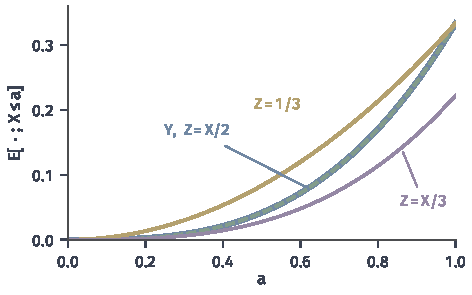
\includegraphics[width=80mm]{figures/07-probability/02-measure-theoretic-probability/matplotlib/cexp-cumulative-check/figure.pdf}
  \caption{用积分刻画检验候选，三角形模型。横轴为$a$，纵轴为事件$\{X\leq a\}$上的累计期望。蓝线是$Y$的$a^{3}/3$，绿色虚线是候选$Z=X/2$，两者重合；黄线是常数候选$1/3$，紫线是候选$X/3$，都与蓝线分离。}
  \label{fig:cexp-cumulative-check}
\end{BookInlineFigure}

\subsection{存在性与唯一性}
\label{sec:cexp-existence}

定义只列出要求，还没有说明满足要求的随机变量是否存在、有几个。有限划分时，式~\eqref{eq:cexp-partition}给出了一个解，零概率组上的任意取值又说明解可能不止一个。一般的$\mathcal{G}$没有组可以逐个处理，需要另找办法。

\paragraph{累计期望是一个测度}
关键是换一个角度看式~\eqref{eq:cexp-defining}的右边。先设$X\geq0$且可积，对$A\in\mathcal{G}$令
\[
 \nu(A)=\mathbb{E}[X\mathbf{1}_{A}] .
\]
$\nu$把每个已知事件对应到$X$在其上的累计期望，可以想成把“$X$的质量”分配到已知事件上。式~\eqref{eq:cexp-defining}要求找一个$\mathcal{G}$可测的$Z$，使$\nu(A)=\mathbb{E}[Z\mathbf{1}_A]$：$Z$是$\nu$相对于$\mathbb{P}$的密度，而且这个密度只能用$\mathcal{G}$中的信息。卷四的Radon--Nikodym定理回答的正是这样的问题：$\sigma$有限测度$\nu$关于$\mu$绝对连续时，存在非负可测函数$h$，使$\nu(A)=\int_A h\,\mathrm{d}\mu$对一切可测集成立，并且$h$在$\mu$几乎处处的意义下唯一，可参考\BookChapterRef{chap:measure-densities}{卷四第8章“测度的密度”}。

图~\ref{fig:cexp-rn-cumulative}用逐次等分的例子展示这个视角。在整个$\mathcal{F}$上，
\[
 \nu([0,t))=\int_0^t\omega^{2}\,\mathrm{d}\omega=\frac{t^{3}}{3},
\]
这条蓝色曲线的斜率就是$X$本身：在$\mathcal{F}$上，$\nu$的密度是$X$。若只允许使用$\mathcal{G}_2$中的事件，$\nu$只在四段及其并上有定义，四段上的质量是
\[
 \begin{gathered}
 \nu(A_1)=\tfrac{1}{192},\qquad \nu(A_2)=\tfrac{7}{192},\\ \nu(A_3)=\tfrac{19}{192},\qquad \nu(A_4)=\tfrac{37}{192},
 \end{gathered}
\]
其中$A_1,\dots,A_4$依次是四个区间。$\mathcal{G}_2$可测的密度在每段上只能取常数，它在$A_i$上必须等于比值$\nu(A_i)/\mathbb{P}(A_i)$，也就是折线在各段的斜率$1/48$、$7/48$、$19/48$、$37/48$，正是第~\ref{sec:cexp-finite-partition}节算出的条件平均。

\begin{BookInlineFigure}
  \centering
  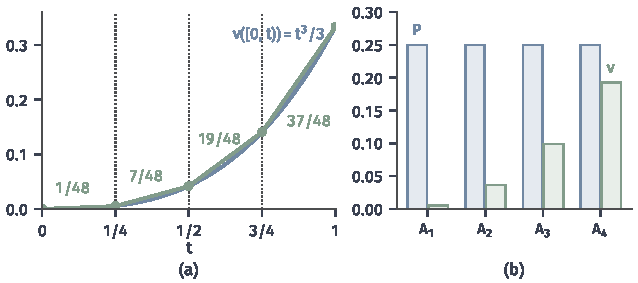
\includegraphics[width=108mm]{figures/07-probability/02-measure-theoretic-probability/matplotlib/cexp-rn-cumulative/figure.pdf}
  \caption{条件期望是限制在$\mathcal{G}$上的密度，$\Omega=[0,1)$，$X(\omega)=\omega^{2}$，$\mathcal{G}=\mathcal{G}_2$。(a)蓝线是$\nu([0,t))=t^{3}/3$，斜率为$X$；绿色折线只经过四个分点，各段斜率是$\mathbb{E}[X\mid\mathcal{G}_2]$的取值。(b)四个区间上$\mathbb{P}(A_i)=1/4$（蓝）与$\nu(A_i)$（绿）的比较，两者之比就是各段斜率。}
  \label{fig:cexp-rn-cumulative}
\end{BookInlineFigure}

\paragraph{存在与唯一}
有了这个视角，存在性归结为在可测空间$(\Omega,\mathcal{G})$上使用Radon--Nikodym定理。唯一性则只用到式~\eqref{eq:cexp-defining}对足够多的事件成立。

\begin{theorem}[条件期望的存在与唯一]
\label{thm:cexp-existence}
设$X$可积，$\mathcal{G}\subseteq\mathcal{F}$是$\sigma$代数。则$X$给定$\mathcal{G}$的条件期望存在。若$Z$与$Z'$都是它的版本，则$Z=Z'$几乎必然成立；反过来，若$Z$是一个版本，$Z'$是$\mathcal{G}$可测的随机变量且$Z'=Z$几乎必然成立，则$Z'$也是一个版本。
\end{theorem}

\begin{proof}
\emph{第一步，非负的$X$。}设$X\geq0$且可积，对$A\in\mathcal{G}$令$\nu(A)=\mathbb{E}[X\mathbf{1}_{A}]$。$\nu(\emptyset)=0$；若$A_1,A_2,\dots\in\mathcal{G}$两两不交，则
\[
 X\mathbf{1}_{\bigcup_nA_n}=\sum_nX\mathbf{1}_{A_n},
\]
右边各项非负，由单调收敛定理，
\[
 \nu\Bigl(\bigcup_nA_n\Bigr)=\sum_n\nu(A_n).
\]
所以$\nu$是$(\Omega,\mathcal{G})$上的测度，总质量$\nu(\Omega)=\mathbb{E}[X]<\infty$。

记$\mathbb{P}_{\mathcal{G}}$为$\mathbb{P}$限制在$\mathcal{G}$上得到的概率测度。若$A\in\mathcal{G}$且$\mathbb{P}(A)=0$，则$X\mathbf{1}_{A}$只在零概率集上非零，$\nu(A)=0$，即$\nu\ll\mathbb{P}_{\mathcal{G}}$。两个测度都有限，由Radon--Nikodym定理，存在$\mathcal{G}$可测的$Z:\Omega\to[0,\infty)$，使
\[
 \nu(A)=\int_{A}Z\,\mathrm{d}\mathbb{P}_{\mathcal{G}},\qquad A\in\mathcal{G}.
\]

右边是对$\mathbb{P}_{\mathcal{G}}$的积分，需要把它换成对$\mathbb{P}$的积分。对$\mathcal{G}$中事件的示性函数，两者都是$\mathbb{P}(A)$；由线性，对$\mathcal{G}$可测的非负简单函数两者相等；非负$\mathcal{G}$可测函数可以由这样的简单函数单调逼近，由单调收敛定理两者仍相等。于是
\[
 \mathbb{E}[Z\mathbf{1}_{A}]=\nu(A)=\mathbb{E}[X\mathbf{1}_{A}],\qquad A\in\mathcal{G}.
\]
取$A=\Omega$得$\mathbb{E}[Z]=\mathbb{E}[X]<\infty$，$Z$可积。$Z$满足定义的三条要求。

\emph{第二步，一般的$X$。}把$X$拆成$X=X^{+}-X^{-}$，两部分非负且可积。由第一步取版本$Z_{+}$与$Z_{-}$，令$Z=Z_{+}-Z_{-}$。它是$\mathcal{G}$可测且可积的，对$A\in\mathcal{G}$，由期望的线性，
\[
 \mathbb{E}[Z\mathbf{1}_{A}]=\mathbb{E}[X^{+}\mathbf{1}_{A}]-\mathbb{E}[X^{-}\mathbf{1}_{A}]=\mathbb{E}[X\mathbf{1}_{A}] .
\]

\emph{第三步，唯一性。}设$Z,Z'$都是版本。两者都$\mathcal{G}$可测，所以$A=\{Z>Z'\}\in\mathcal{G}$。由式~\eqref{eq:cexp-defining}，
\[
 \mathbb{E}\bigl[(Z-Z')\mathbf{1}_{A}\bigr]=\mathbb{E}[X\mathbf{1}_{A}]-\mathbb{E}[X\mathbf{1}_{A}]=0 .
\]
被积函数$(Z-Z')\mathbf{1}_{A}$非负而期望为零，所以它几乎必然为零；它在$A$上严格为正，于是$\mathbb{P}(A)=0$。交换$Z$与$Z'$得$\mathbb{P}(Z'>Z)=0$，所以$Z=Z'$几乎必然成立。

最后，若$Z'$是$\mathcal{G}$可测的且$Z'=Z$几乎必然成立，则$Z'$可积，并且对每个$A$，$Z'\mathbf{1}_{A}$与$Z\mathbf{1}_{A}$几乎必然相等，期望相同，所以$Z'$也满足式~\eqref{eq:cexp-defining}。
\end{proof}

\paragraph{版本与几乎必然}
定理说明，条件期望是一个只确定到零概率集的对象：不同版本可以在一个零概率集上取不同的值，除此之外完全一样。这与有限划分中零概率组上的任意常数是同一回事。所以，凡是关于$\mathbb{E}[X\mid\mathcal{G}]$的等式和不等式，都按几乎必然的意义理解，并且对它的任何一个版本都成立；后文不再逐次声明。

修改一个版本时要注意可测性。改动后的随机变量必须仍是$\mathcal{G}$可测的；若$\mathcal{G}$不含某个零概率集的全部子集，在其上随意改值可能破坏这一点，这时定理的最后一句不能使用。第~\ref{chap:probability-spaces}章的完备化可以消除这类麻烦，但条件期望的定义并不依赖它。

第~\ref{sec:cexp-prediction}节还会给出另一条构造路线：当$X$平方可积时，条件期望是一个正交投影。那条路线只适用于平方可积的变量，一般的可积变量仍由上面的定理保证。

\subsection{给定随机变量的条件期望}
\label{sec:cexp-given-variable}

\paragraph{给定观测的条件期望}
最常见的信息来自一个观测。设$Y$是取值于$\mathbb{R}^{k}$的随机向量，或者更一般地，取值于某个可测空间$(E,\mathcal{E})$的随机对象。第~\ref{chap:probability-spaces}章定义了它生成的$\sigma$代数
\[
 \sigma(Y)=\bigl\{\{Y\in B\}:\ B\in\mathcal{E}\bigr\},
\]
它由所有“能凭$Y$的值判断是否发生”的事件组成。对可积的$X$，定义
\begin{equation}
 \mathbb{E}[X\mid Y]=\mathbb{E}\bigl[X\mid\sigma(Y)\bigr].
 \label{eq:cexp-given-variable}
\end{equation}
给定几个观测$Y_1,\dots,Y_k$时，把它们合成一个随机向量$(Y_1,\dots,Y_k)$。

在传感器表中，$\mathbb{E}[Y\mid X]=m(X)$是$X$的函数。一般情形下，$\sigma(Y)$可测的随机变量是否也都能写成$Y$的函数？直观上应当如此：$\sigma(Y)$可测意味着样本点只要$Y$值相同，取值就相同，见图~\ref{fig:cexp-factorization}。下面的\term{因子分解引理}（factorization lemma）把这一点写准。

\begin{BookInlineFigure}
  \centering
  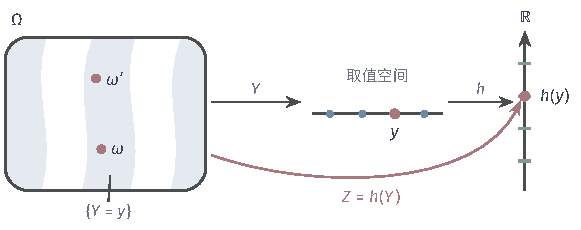
\includegraphics[width=98mm]{figures/07-probability/02-measure-theoretic-probability/tikz/cexp-factorization/figure.pdf}
  \caption{经由观测的因子分解。左边$\Omega$被分成水平集$\{Y=y\}$（浅蓝与白色条带）；同一条带内的$\omega$与$\omega'$有相同的$Y$值，因而$\sigma(Y)$可测的$Z$在两点取值相同。于是$Z$可以先经$Y$映到取值空间，再经可测函数$h$映到$\mathbb{R}$，即$Z=h(Y)$。}
  \label{fig:cexp-factorization}
\end{BookInlineFigure}

\begin{lemma}[因子分解引理]
\label{lem:cexp-factorization}
设$Y:\Omega\to E$关于$\mathcal{E}$可测，$Z:\Omega\to\mathbb{R}$关于$\sigma(Y)$可测。则存在可测函数$h:E\to\mathbb{R}$，使$Z=h(Y)$在$\Omega$上处处成立。
\end{lemma}

\begin{proof}
先设$Z$是示性函数$\mathbf{1}_{A}$，$A\in\sigma(Y)$。由$\sigma(Y)$的定义，有$B\in\mathcal{E}$使$A=\{Y\in B\}$，于是
\[
 Z=\mathbf{1}_{B}(Y),
\]
取$h=\mathbf{1}_{B}$即可。若$Z$是有限个这样的示性函数的线性组合$\sum_{i}a_i\mathbf{1}_{A_i}$，对每个$A_i$取对应的$B_i$，令$h=\sum_ia_i\mathbf{1}_{B_i}$。

一般情形，取$\sigma(Y)$可测的简单函数$Z_n$，使$Z_n(\omega)\to Z(\omega)$对每个$\omega$成立；例如把$\max(-n,\min(Z,n))$向零截断到$2^{-n}$的整数倍。由上一段，$Z_n=h_n(Y)$，$h_n$可测。令
\[
 L=\bigl\{e\in E:\ \lim_{n\to\infty}h_n(e)\ \text{存在且有限}\bigr\},
\]
它是$\limsup_nh_n$与$\liminf_nh_n$相等且有限的点集，因而可测；在$L$上令$h=\lim_nh_n$，在$L$外令$h=0$，$h$可测。对每个$\omega$，数列$h_n(Y(\omega))=Z_n(\omega)$收敛到$Z(\omega)$，所以$Y(\omega)\in L$，并且$h(Y(\omega))=Z(\omega)$。
\end{proof}

把引理用于$\mathbb{E}[X\mid Y]$的任一版本，得到可测函数$m:E\to\mathbb{R}$，使
\begin{equation}
 \mathbb{E}[X\mid Y]=m(Y).
 \label{eq:cexp-regression-function}
\end{equation}
按惯例记$\mathbb{E}[X\mid Y=y]=m(y)$。由于$\sigma(Y)$中的事件都是$\{Y\in B\}$，并且$\mathbb{E}[m(Y)\mathbf{1}_B(Y)]$可以用推前分布写成对$P_Y$的积分，一个可测函数$m$满足要求，当且仅当$m(Y)$可积，并且对每个$B\in\mathcal{E}$，
\begin{equation}
 \mathbb{E}\bigl[X\mathbf{1}_{\{Y\in B\}}\bigr]=\int_{B}m(y)\,P_Y(\mathrm{d}y).
 \label{eq:cexp-given-variable-check}
\end{equation}

\paragraph{函数只在分布下几乎处处确定}
$m(Y)$与$m(y)$要分清。前者是$\Omega$上的随机变量，作为条件期望的版本，几乎必然唯一；后者是取值空间上的普通函数。两个函数$m,\tilde m$都满足要求，当且仅当$m(Y)=\tilde m(Y)$几乎必然成立，也就是
\[
 P_Y\bigl(\{y:\ m(y)\neq\tilde m(y)\}\bigr)=\mathbb{P}\bigl(m(Y)\neq\tilde m(Y)\bigr)=0 .
\]
所以$m$只在$P_Y$几乎处处的意义下确定：在$Y$取不到的地方，$m$可以任意取值；在$Y$以零概率取到的单个点上，$m$的值也没有意义。

“只知绝对值”的例子把这一点画得很清楚。$Y=\lvert X\rvert\sim\operatorname{Unif}(0,1)$，$m(y)=y/2$是$\mathbb{E}[X^{+}\mid Y=y]$的一个版本。把$m$在$y=1/2$处改成$0.9$，并在$[0,1]$之外任意改动，得到的$\tilde m$仍是一个版本，见图~\ref{fig:cexp-versions}(a)。在$\Omega$上看，$\tilde m(Y)$与$m(Y)$只在$\omega=\pm1/2$两点不同，见图~\ref{fig:cexp-versions}(b)。问“已知$\lvert X\rvert=1/2$时$X^{+}$的平均是多少”，单凭条件期望的定义无法回答；要给单个观测值指定确定的条件平均，需要额外的要求，例如$m$的连续性，这在第~\ref{chap:conditional-distributions}章讨论。

\begin{BookInlineFigure}
  \centering
  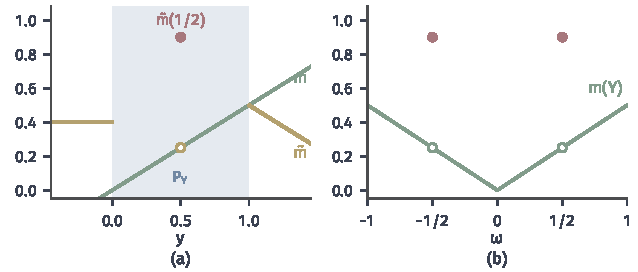
\includegraphics[width=108mm]{figures/07-probability/02-measure-theoretic-probability/matplotlib/cexp-versions/figure.pdf}
  \caption{$\mathbb{E}[X^{+}\mid Y]$的两个版本，$Y=\lvert X\rvert$，$X\sim\operatorname{Unif}(-1,1)$。(a)绿线$m(y)=y/2$；黄线与红点组成的$\tilde m$在$[0,1]$上只在$y=1/2$处不同，在浅蓝区间$[0,1]$（$P_Y$所在之处）以外任意取值。(b)复合到$\Omega$上，$\tilde m(Y)$与$m(Y)$只在$\omega=\pm1/2$两点（红点）不同。}
  \label{fig:cexp-versions}
\end{BookInlineFigure}

\paragraph{回到条件均值的公式}
式~\eqref{eq:cexp-given-variable-check}说明，第~\ref{chap:random-vectors}章的两个公式都给出了版本。若$Y$只取可数多个值，对$\mathbb{P}(Y=y)>0$的$y$令
\[
 m(y)=\frac{\mathbb{E}\bigl[X\mathbf{1}_{\{Y=y\}}\bigr]}{\mathbb{P}(Y=y)},
\]
其余$y$上任意取值。两边对$B$中的$y$求和，式~\eqref{eq:cexp-given-variable-check}成立，交换求和与期望由$\mathbb{E}\lvert X\rvert<\infty$保证。

若$(X,Y)$有联合密度$f_{X,Y}$，$Y$为实值，在$f_Y(y)>0$处令
\[
 m(y)=\frac{1}{f_Y(y)}\int x\,f_{X,Y}(x,y)\,\mathrm{d}x ,
\]
其余$y$上令$m(y)=0$。由$\mathbb{E}\lvert X\rvert<\infty$与Fubini定理，
\[
 \mathbb{E}\bigl[X\mathbf{1}_{\{Y\in B\}}\bigr]=\int_{B}\int x\,f_{X,Y}(x,y)\,\mathrm{d}x\,\mathrm{d}y=\int_{B}m(y)f_Y(y)\,\mathrm{d}y ,
\]
这正是式~\eqref{eq:cexp-given-variable-check}。$f_Y(y)=0$的那些$y$对右边没有贡献，$m$在那里怎样取都可以。

没有密度时，可以像前面那样直接验证候选。在“只知绝对值”的例子中，对满足$\mathbb{E}\lvert g(X)\rvert<\infty$的可测函数$g$，把积分按$\pm x$配对，
\[
 \mathbb{E}\bigl[g(X)\mathbf{1}_{\{Y\in B\}}\bigr]
 =\int_{0}^{1}\frac{g(y)+g(-y)}{2}\,\mathbf{1}_{B}(y)\,\mathrm{d}y .
\]
右边正是式~\eqref{eq:cexp-given-variable-check}，其中$P_Y$是$[0,1]$上的均匀分布，所以
\begin{equation}
 \mathbb{E}\bigl[g(X)\bigm|\lvert X\rvert\bigr]=\frac{g(\lvert X\rvert)+g(-\lvert X\rvert)}{2}.
 \label{eq:cexp-folding}
\end{equation}
取$g(x)=x^{+}$得到$\lvert X\rvert/2$；取$g(x)=x$得到$0$；取$g(x)=\mathrm{e}^{x}$得到$\cosh\lvert X\rvert$，见图~\ref{fig:cexp-folding}(b)。


\section{基本性质}
\label{sec:cexp-properties}

有了定义，下一步是学会运算。在有限分组中，组内平均对随机变量是线性的、保序的，已经知道的量在组内是常数，可以提到平均号外面。这些性质在一般的$\mathcal{G}$下是否仍然成立？本节固定信息$\mathcal{G}$，逐条从积分定义核验它们，并用传感器表检验计算含义。核验的办法都相同：写出候选，检查它$\mathcal{G}$可测、可积，并在每个$A\in\mathcal{G}$上满足式~\eqref{eq:cexp-defining}，再由定理~\ref{thm:cexp-existence}的唯一性得出几乎必然相等。最后讨论另一种极端：当信息与变量独立时，条件平均就是普通的平均。

\subsection{线性与保序}
\label{sec:cexp-linearity}

先看两条最基本的规则。在每一组内求平均，和的平均是平均的和，较大变量的平均不小于较小变量的平均。下面的定理说明它们对一般信息仍然成立，只是相等与不等都按几乎必然理解。

\begin{theorem}[线性与保序]
\label{thm:cexp-linearity}
设$X_1,X_2$可积，$a,b$是实数。则
\begin{equation}
 \mathbb{E}[aX_1+bX_2\mid\mathcal{G}]=a\,\mathbb{E}[X_1\mid\mathcal{G}]+b\,\mathbb{E}[X_2\mid\mathcal{G}].
 \label{eq:cexp-linearity}
\end{equation}
若$X_1\leq X_2$几乎必然成立，则
\begin{equation}
 \mathbb{E}[X_1\mid\mathcal{G}]\leq\mathbb{E}[X_2\mid\mathcal{G}].
 \label{eq:cexp-monotone}
\end{equation}
特别地，常数$c$满足$\mathbb{E}[c\mid\mathcal{G}]=c$，并且
\begin{equation}
 \bigl\lvert\mathbb{E}[X_1\mid\mathcal{G}]\bigr\rvert\leq\mathbb{E}\bigl[\lvert X_1\rvert\bigm|\mathcal{G}\bigr].
 \label{eq:cexp-abs}
\end{equation}
\end{theorem}

\begin{proof}
记$Z_1,Z_2$为$X_1,X_2$的条件期望的版本。

\emph{线性。}$aZ_1+bZ_2$是$\mathcal{G}$可测的可积函数。对$A\in\mathcal{G}$，由期望的线性和式~\eqref{eq:cexp-defining}，
\[
 \mathbb{E}\bigl[(aZ_1+bZ_2)\mathbf{1}_{A}\bigr]
 =a\,\mathbb{E}[X_1\mathbf{1}_{A}]+b\,\mathbb{E}[X_2\mathbf{1}_{A}]
 =\mathbb{E}\bigl[(aX_1+bX_2)\mathbf{1}_{A}\bigr].
\]
所以$aZ_1+bZ_2$是$aX_1+bX_2$的条件期望的一个版本，由唯一性得式~\eqref{eq:cexp-linearity}。

\emph{非负性。}先设$X\geq0$几乎必然成立，$Z$是$\mathbb{E}[X\mid\mathcal{G}]$的版本。事件$A=\{Z<0\}$属于$\mathcal{G}$，于是
\[
 \mathbb{E}[Z\mathbf{1}_{A}]=\mathbb{E}[X\mathbf{1}_{A}]\geq0 .
\]
另一方面$Z\mathbf{1}_{A}\leq0$，期望不大于零。两者合起来，$Z\mathbf{1}_{A}$是期望为零的非正函数，几乎必然为零；它在$A$上严格为负，所以$\mathbb{P}(A)=0$，即$Z\geq0$几乎必然成立。

\emph{保序。}对$X_2-X_1\geq0$用非负性，再用线性，得式~\eqref{eq:cexp-monotone}。由$-\lvert X_1\rvert\leq X_1\leq\lvert X_1\rvert$与保序，得到绝对值的不等式。常数$c$本身是$\mathcal{G}$可测的，满足定义的三条要求。
\end{proof}

线性对应于“组内平均可以逐项计算”，保序对应于“逐点更大的量，组内平均也更大”。在传感器表上，$\mathbb{E}[2Y-1\mid X]=2\,\mathbb{E}[Y\mid X]-1$，三行依次是
\[
 2\cdot\tfrac13-1=-\tfrac13,\qquad 2\cdot1-1=1,\qquad 2\cdot\tfrac53-1=\tfrac73 ,
\]
与直接按行求$2Y-1$的平均相同。又因为$0\leq Y\leq2$，保序给出$0\leq\mathbb{E}[Y\mid X]\leq2$，三个行均值确实落在这个范围。

“几乎必然”在这里有一个实际后果。式~\eqref{eq:cexp-linearity}对每一对$(X_1,X_2)$和每一对系数，都在一个可能依赖于它们的零概率集之外成立。对可数多个这样的等式，把例外集并起来仍是零概率集，可以同时使用；对不可数多个，例如对所有实数$a$同时成立，就不能直接合并例外集。逐事件的条件概率要拼成一个完整的分布，正卡在这一点上，第~\ref{chap:conditional-distributions}章会处理它。

\subsection{提取已知量}
\label{sec:cexp-known}

\paragraph{已知的乘子可以提出}
在一组之内，$\mathcal{G}$可测的量是常数，常数可以从平均里提出来。传感器表中，给定$X$时$X$已知，所以应当有$\mathbb{E}[XY\mid X]=X\,\mathbb{E}[Y\mid X]$。这条规则称为\term{提取已知量}（taking out what is known）。下面的定理说明它对一般信息成立，并说明乘子需要满足什么条件。

\begin{theorem}[提取已知量]
\label{thm:cexp-known}
设$H$是$\mathcal{G}$可测的随机变量，$X$与$HX$都可积。则$H\,\mathbb{E}[X\mid\mathcal{G}]$可积，并且
\begin{equation}
 \mathbb{E}[HX\mid\mathcal{G}]=H\,\mathbb{E}[X\mid\mathcal{G}].
 \label{eq:cexp-known}
\end{equation}
特别地，若$H$是$\mathcal{G}$可测且可积的，则$\mathbb{E}[H\mid\mathcal{G}]=H$。
\end{theorem}

证明分三步扩大乘子的范围：先是示性函数，再是有界函数，最后是一般函数。前两步是定义的直接推论；最后一步的难点在于，事先并不知道$HZ$可积，不能直接用控制收敛定理，需要先对非负的情形用单调收敛定理得到可积性。

\begin{proof}
记$Z=\mathbb{E}[X\mid\mathcal{G}]$。$HZ$是两个$\mathcal{G}$可测函数之积，本身$\mathcal{G}$可测。由唯一性，只需证明$HZ$可积，并且对每个$A\in\mathcal{G}$，
\[
 \mathbb{E}[HX\mathbf{1}_{A}]=\mathbb{E}[HZ\mathbf{1}_{A}] .
\]

\emph{第一步，示性函数与简单函数。}设$H=\mathbf{1}_{B}$，$B\in\mathcal{G}$。$A\cap B\in\mathcal{G}$，由式~\eqref{eq:cexp-defining}，
\[
 \mathbb{E}[\mathbf{1}_{B}X\mathbf{1}_{A}]=\mathbb{E}[X\mathbf{1}_{A\cap B}]=\mathbb{E}[Z\mathbf{1}_{A\cap B}]=\mathbb{E}[\mathbf{1}_{B}Z\mathbf{1}_{A}] .
\]
由线性，结论对$\mathcal{G}$可测的简单函数$H$成立。

\emph{第二步，有界的$H$。}设$\lvert H\rvert\leq c$。取$\mathcal{G}$可测的简单函数$H_n$，使$\lvert H_n\rvert\leq c$且$H_n\to H$逐点成立。由第一步，
\[
 \mathbb{E}[H_nX\mathbf{1}_{A}]=\mathbb{E}[H_nZ\mathbf{1}_{A}] .
\]
左边被积函数被$c\lvert X\rvert$控制，右边被$c\lvert Z\rvert$控制，两者都可积。由控制收敛定理令$n\to\infty$，两边分别趋于$\mathbb{E}[HX\mathbf{1}_{A}]$与$\mathbb{E}[HZ\mathbf{1}_{A}]$。

\emph{第三步，非负的$H$与$X$。}设$H\geq0$，$X\geq0$，于是$Z\geq0$。令$H_n=\min(H,n)$，由第二步，
\[
 \mathbb{E}[H_nX\mathbf{1}_{A}]=\mathbb{E}[H_nZ\mathbf{1}_{A}] .
\]
两边的被积函数都非负并且随$n$单调增加，由单调收敛定理令$n\to\infty$，得到
\[
 \mathbb{E}[HX\mathbf{1}_{A}]=\mathbb{E}[HZ\mathbf{1}_{A}] .
\]
取$A=\Omega$，左边是有限的$\mathbb{E}[HX]$，所以$HZ$可积。

\emph{第四步，一般情形。}写$H=H^{+}-H^{-}$，$X=X^{+}-X^{-}$，并记$Z_{\pm}=\mathbb{E}[X^{\pm}\mid\mathcal{G}]$，于是$Z=Z_{+}-Z_{-}$。四个乘积$H^{\pm}X^{\pm}$都被$\lvert HX\rvert$控制，因而可积。对每一对符号用第三步，得到$H^{\pm}Z_{\pm}$可积，且
\[
 \mathbb{E}[H^{\pm}X^{\pm}\mathbf{1}_{A}]=\mathbb{E}[H^{\pm}Z_{\pm}\mathbf{1}_{A}] .
\]
把四个等式按$HX=(H^{+}-H^{-})(X^{+}-X^{-})$的符号相加，右边合成$\mathbb{E}[HZ\mathbf{1}_{A}]$，左边合成$\mathbb{E}[HX\mathbf{1}_{A}]$；而$\lvert HZ\rvert$不超过四个可积函数$H^{\pm}Z_{\pm}$之和，所以$HZ$可积。

最后一句取$X=1$：$\mathbb{E}[1\mid\mathcal{G}]=1$，$H\cdot1$可积，于是$\mathbb{E}[H\mid\mathcal{G}]=H$。
\end{proof}

定理要求$HX$可积，否则左边的条件期望在本章的意义下没有定义。乘子本身不必有界：$X$与$HX$可积就够了，结论里$H\,\mathbb{E}[X\mid\mathcal{G}]$的可积性是证明出来的，不是假设的。

\paragraph{传感器表上的计算}
在传感器表中取$H=X$，它是$\sigma(X)$可测的。由式~\eqref{eq:cexp-known}与三行的条件均值，
\[
 \mathbb{E}[XY\mid X]=X\,\mathbb{E}[Y\mid X]:\qquad 0\cdot\tfrac13=0,\qquad 1\cdot1=1,\qquad 2\cdot\tfrac53=\tfrac{10}{3},
\]
见图~\ref{fig:cexp-known-factor}(a)。直接计算第三行核对：第三行中$Y$以条件概率$\tfrac13,\tfrac23$取$1,2$，$XY$取$2,4$，平均为$\tfrac23+\tfrac83=\tfrac{10}{3}$。

\begin{BookInlineFigure}
  \centering
  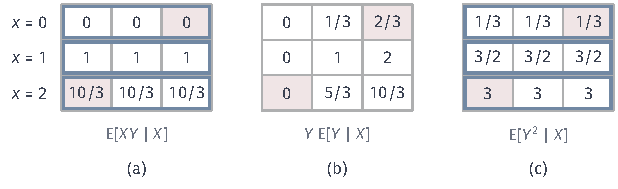
\includegraphics[width=104mm]{figures/07-probability/02-measure-theoretic-probability/tikz/cexp-known-factor/figure.pdf}
  \caption{提取已知量，传感器表，浅红格的概率为零。(a)$\mathbb{E}[XY\mid X]=X\,\mathbb{E}[Y\mid X]$，每行取常数$0$、$1$、$10/3$（蓝框表示行内为常数）。(b)$Y\,\mathbb{E}[Y\mid X]$在同一行内变化，不是$X$的函数。(c)$\mathbb{E}[Y^{2}\mid X]$，每行取$1/3$、$3/2$、$3$。}
  \label{fig:cexp-known-factor}
\end{BookInlineFigure}

\paragraph{未知的乘子不能提出}
乘子必须是已知的。若把$Y$当作乘子，“$\mathbb{E}[Y\cdot Y\mid X]=Y\,\mathbb{E}[Y\mid X]$”就是错的。右边在同一行内随$Y$变化，见图~\ref{fig:cexp-known-factor}(b)，它不是$\sigma(X)$可测的，根本不可能是给定$X$的条件期望。正确的值由行内平均给出：
\[
 \mathbb{E}[Y^{2}\mid X=0]=\tfrac13,\qquad \mathbb{E}[Y^{2}\mid X=1]=\tfrac32,\qquad \mathbb{E}[Y^{2}\mid X=2]=3 ,
\]
见图~\ref{fig:cexp-known-factor}(c)。例如第二行中$Y^{2}$以$\tfrac14,\tfrac12,\tfrac14$取$0,1,4$，平均为$\tfrac12+1=\tfrac32$。在组内，已知量是常数，未知量仍在变化；只有前者能提到平均号外面。

\subsection{独立情形}
\label{sec:cexp-independence}

\paragraph{与信息独立的变量}
如果已知的信息与$X$毫无关联，给定这份信息的平均就不应改变。称$X$与$\mathcal{G}$独立，是指对每个Borel集$B$与每个$A\in\mathcal{G}$，事件$\{X\in B\}$与$A$独立，也就是$\sigma(X)$与$\mathcal{G}$独立。这时$X$与每个$\mathbf{1}_{A}$是独立的随机变量，由第~\ref{chap:probability-spaces}章的积分表示，两个独立可积变量乘积的期望等于期望的乘积。

\begin{theorem}[独立的信息]
\label{thm:cexp-independent}
设$X$可积并且与$\mathcal{G}$独立。则
\begin{equation}
 \mathbb{E}[X\mid\mathcal{G}]=\mathbb{E}[X].
 \label{eq:cexp-independent}
\end{equation}
\end{theorem}

\begin{proof}
常数$\mathbb{E}[X]$是$\mathcal{G}$可测且可积的。对$A\in\mathcal{G}$，$X$与$\mathbf{1}_{A}$独立且都可积，乘积的期望等于期望的乘积，
\[
 \mathbb{E}[X\mathbf{1}_{A}]=\mathbb{E}[X]\,\mathbb{P}(A)=\mathbb{E}\bigl[\mathbb{E}[X]\,\mathbf{1}_{A}\bigr].
\]
所以常数$\mathbb{E}[X]$满足式~\eqref{eq:cexp-defining}。
\end{proof}

“只知绝对值”的例子提供了一个独立的情形。记$S=\operatorname{sgn}X$，它以各$\tfrac12$的概率取$\pm1$。对$0\leq t\leq1$，
\[
 \mathbb{P}\bigl(S=1,\ \lvert X\rvert\leq t\bigr)=\mathbb{P}(0<X\leq t)=\frac t2=\mathbb{P}(S=1)\,\mathbb{P}\bigl(\lvert X\rvert\leq t\bigr),
\]
所以符号与绝对值独立。由定理~\ref{thm:cexp-independent}，$\mathbb{E}[S\mid\lvert X\rvert]=\mathbb{E}[S]=0$：知道离原点多远，对“在哪一侧”毫无帮助。再由$X=S\lvert X\rvert$与提取已知量，
\[
 \mathbb{E}\bigl[X\bigm|\lvert X\rvert\bigr]=\lvert X\rvert\,\mathbb{E}\bigl[S\bigm|\lvert X\rvert\bigr]=0 ,
\]
与式~\eqref{eq:cexp-folding}取$g(x)=x$的结果一致。

\paragraph{条件平均为常数不能推出独立}
定理~\ref{thm:cexp-independent}的逆命题不成立。上面刚得到$\mathbb{E}[X\mid\lvert X\rvert]=0=\mathbb{E}[X]$，可是$X$与$\lvert X\rvert$不独立，取一对事件就能看出：
\[
 \mathbb{P}\bigl(\lvert X\rvert\leq\tfrac12,\ X>\tfrac12\bigr)=0,\qquad
 \mathbb{P}\bigl(\lvert X\rvert\leq\tfrac12\bigr)\,\mathbb{P}\bigl(X>\tfrac12\bigr)=\tfrac12\cdot\tfrac14=\tfrac18 .
\]
图~\ref{fig:cexp-independence}比较了两种情形。左边给定$\lvert X\rvert=y$后，$X$只能是$\pm y$，条件规律随$y$剧烈变化，只是两点的平均恰好总为$0$；右边$Z$与$X$独立，给定$Z$后$X$的整个分布都不变。两者的条件平均都是常数$0$，图中的红线完全相同。

\begin{BookInlineFigure}
  \centering
  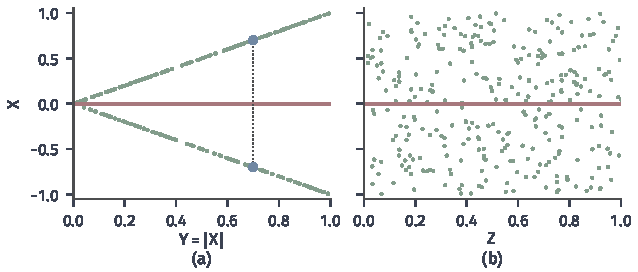
\includegraphics[width=108mm]{figures/07-probability/02-measure-theoretic-probability/matplotlib/cexp-independence/figure.pdf}
  \caption{条件平均为常数不等于独立。随机数种子$7$，各$300$个模拟点（绿）。(a)$X\sim\operatorname{Unif}(-1,1)$与$Y=\lvert X\rvert$，点落在两条线段$x=\pm y$上；给定$Y=0.7$时$X$只取蓝点$\pm0.7$，条件平均为$0$（红线）。(b)$X\sim\operatorname{Unif}(-1,1)$与独立的$Z\sim\operatorname{Unif}(0,1)$，点铺满矩形，条件平均同样为$0$。}
  \label{fig:cexp-independence}
\end{BookInlineFigure}

条件平均为常数只约束一个数：每组的平均都等于总平均。独立则要求给定信息后$X$落在任何集合中的条件概率都不变，即对一切Borel集$B$，
\[
 \mathbb{E}\bigl[\mathbf{1}_{\{X\in B\}}\bigm|\mathcal{G}\bigr]=\mathbb{P}(X\in B).
\]
前者只要求$X$本身的条件平均不变，后者要求每个示性函数$\mathbf{1}_{\{X\in B\}}$的条件平均都不变，由后者可以推出前者。给定信息后完整的条件规律在第~\ref{chap:conditional-distributions}章研究，那里的条件独立也要求整个条件分布满足乘积关系，而不只是条件均值。


\section{迭代条件期望}
\label{sec:cexp-iterated}

条件期望$\mathbb{E}[X\mid\mathcal{G}]$本身是一个可积的随机变量，可以再对它求期望，或者再给定另一份信息求条件期望。这样平均两次，结果是什么？分两种情况：一种是第二次什么也不给定，条件被完全取消；另一种是第二次保留另一层信息。后一种情况能否化简，取决于两份信息之间有没有包含关系。

\subsection{全期望公式}
\label{sec:cexp-total-expectation}

\paragraph{先分组平均，再按组加权}
取消条件的情形最简单：在式~\eqref{eq:cexp-defining}中取$A=\Omega$。$\Omega$总在$\mathcal{G}$中，于是得到下面的定理。

\begin{theorem}[全期望公式]
\label{thm:cexp-total-expectation}
设$X$可积，$\mathcal{G}\subseteq\mathcal{F}$是$\sigma$代数。则
\begin{equation}
 \mathbb{E}\bigl[\mathbb{E}[X\mid\mathcal{G}]\bigr]=\mathbb{E}[X].
 \label{eq:cexp-total-expectation}
\end{equation}
\end{theorem}

\begin{proof}
在式~\eqref{eq:cexp-defining}中取$A=\Omega$，$\mathbf{1}_{\Omega}=1$。
\end{proof}

证明只有一行，含义却很具体。在有限划分中，$\mathbb{E}[X\mid\mathcal{G}]$在第$i$组取$c_i$，所以它的期望是$\sum_ic_i\mathbb{P}(A_i)$：先在每一组内求平均，再以各组的概率为权重把组平均加起来，就恢复了总平均。把概率看成质量，这就是“整体的重心等于各部分重心按质量加权的重心”。

传感器表上的计算见图~\ref{fig:cexp-total-expectation}。三行的质量依次是$0.3,0.4,0.3$，行内重心是$1/3,1,5/3$；把每行的质量集中到它的重心，再求这三个点的重心，
\[
 0.3\cdot\tfrac13+0.4\cdot1+0.3\cdot\tfrac53=0.1+0.4+0.5=1=\mathbb{E}[Y].
\]

\begin{BookInlineFigure}
  \centering
  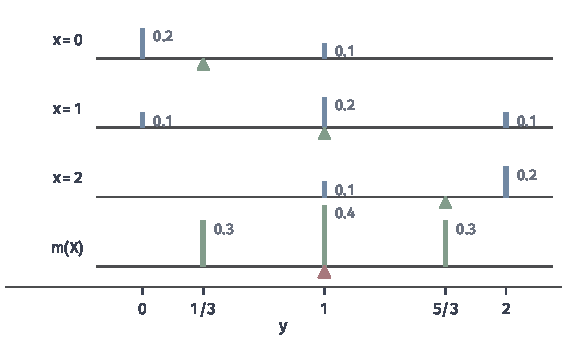
\includegraphics[width=96mm]{figures/07-probability/02-measure-theoretic-probability/matplotlib/cexp-total-expectation/figure.pdf}
  \caption{全期望公式是重心的合成，传感器表。上面三层是三行中的联合质量（蓝色竖线，高度与质量成正比），绿色三角是各行的重心$1/3$、$1$、$5/3$。最下一层把各行的质量$0.3$、$0.4$、$0.3$移到行重心（绿色竖线），它们的重心是$\mathbb{E}[Y]=1$（红色三角）。}
  \label{fig:cexp-total-expectation}
\end{BookInlineFigure}

逐次等分的例子同样可以核对。$\mathcal{G}_2$的四段各占$1/4$，段内平均是$\tfrac{1}{48},\tfrac{7}{48},\tfrac{19}{48},\tfrac{37}{48}$，于是
\[
 \mathbb{E}\bigl[\mathbb{E}[X\mid\mathcal{G}_2]\bigr]=\frac14\cdot\frac{1+7+19+37}{48}=\frac{64}{192}=\frac13=\int_0^1\omega^{2}\,\mathrm{d}\omega .
\]

\paragraph{统一求和与积分}
第~\ref{chap:random-vectors}章分别对概率表和联合密度证明了全期望公式，现在两者都是式~\eqref{eq:cexp-total-expectation}的特例。给定观测$Y$时，$\mathbb{E}[X\mid Y]=m(Y)$，由推前分布的积分公式，
\[
 \mathbb{E}[X]=\mathbb{E}\bigl[m(Y)\bigr]=\int m(y)\,P_Y(\mathrm{d}y).
\]
$Y$只取可数多个值时，右边是$\sum_ym(y)\,p_Y(y)$；$Y$有密度时，右边是$\int m(y)f_Y(y)\,\mathrm{d}y$。两种计算方式只是对$P_Y$积分的两种具体写法。

全期望公式在没有密度时同样好用。“只知绝对值”的例子中，由式~\eqref{eq:cexp-folding}，$\mathrm{e}^{X}$给定$\lvert X\rvert$的条件期望是$\cosh\lvert X\rvert$，而$\lvert X\rvert\sim\operatorname{Unif}(0,1)$，于是
\[
 \mathbb{E}[\mathrm{e}^{X}]=\mathbb{E}\bigl[\cosh\lvert X\rvert\bigr]=\int_0^1\cosh y\,\mathrm{d}y=\sinh 1 .
\]
直接计算得到同样的结果：
\[
 \mathbb{E}[\mathrm{e}^{X}]=\frac12\int_{-1}^{1}\mathrm{e}^{x}\,\mathrm{d}x=\frac{\mathrm{e}-\mathrm{e}^{-1}}{2}=\sinh1 .
\]
先把对称的两点合并，被积函数变成偶函数$\cosh$，积分区间减半；这正是先分组平均、再对组求平均的计算方式。

\subsection{塔式法则}
\label{sec:cexp-tower}

\paragraph{嵌套的信息}
现在第二次平均也保留一些信息。设$\mathcal{H}\subseteq\mathcal{G}$：$\mathcal{H}$中的事件都能由$\mathcal{G}$判断，$\mathcal{H}$是较少的信息。有限划分时，这表示$\mathcal{H}$的每一组都是$\mathcal{G}$的若干组之并，即$\mathcal{G}$是$\mathcal{H}$的细分。

传感器表中取$\mathcal{G}=\sigma(X)$，再取$\mathcal{H}=\sigma(\mathbf{1}_{\{X=2\}})$，后者只知道第一台“是否读偏高”，把前两行并成一组$\{X\leq1\}$，第三行单独一组。先按行平均，再在$\mathcal{H}$的组内平均：$\{X\leq1\}$的概率是$0.7$，其中前两行的质量分别是$0.3$与$0.4$，于是
\[
 \mathbb{E}\bigl[\mathbb{E}[Y\mid X]\bigm|\mathcal{H}\bigr]=\frac{0.3\cdot\frac13+0.4\cdot1}{0.7}=\frac{0.5}{0.7}=\frac57\quad\text{在}\ \{X\leq1\}\ \text{上}.
\]
另一方面，直接在$\{X\leq1\}$上求$Y$的平均，五个正概率格子上的累计期望是$0.1+0.4=0.5$，同样得$5/7$。第三行在两种算法下都是$5/3$。图~\ref{fig:cexp-tower-nested}画出了这两条路径。

\begin{BookInlineFigure}
  \centering
  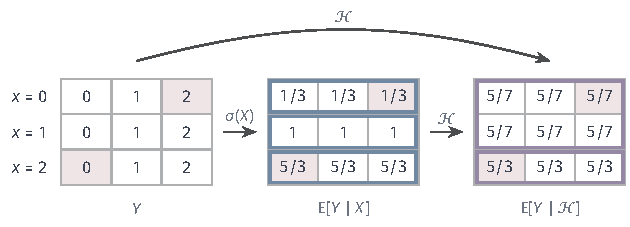
\includegraphics[width=106mm]{figures/07-probability/02-measure-theoretic-probability/tikz/cexp-tower-nested/figure.pdf}
  \caption{嵌套信息下的塔式法则，传感器表，浅红格概率为零。左：$Y$在九个格子上的值。中：$\mathbb{E}[Y\mid X]$，在每行（蓝框）取常数。右：$\mathbb{E}[Y\mid\mathcal{H}]$，$\mathcal{H}=\sigma(\mathbf{1}_{\{X=2\}})$的两组（紫框）上分别取$5/7$与$5/3$。下方两步与上方一步得到相同的结果。}
  \label{fig:cexp-tower-nested}
\end{BookInlineFigure}

\paragraph{先细后粗与先粗后细}
两种顺序都得到较粗信息上的条件期望。

\begin{theorem}[塔式法则]
\label{thm:cexp-tower}
设$X$可积，$\mathcal{H}\subseteq\mathcal{G}\subseteq\mathcal{F}$都是$\sigma$代数。则
\begin{equation}
 \mathbb{E}\bigl[\mathbb{E}[X\mid\mathcal{G}]\bigm|\mathcal{H}\bigr]=\mathbb{E}[X\mid\mathcal{H}]
 =\mathbb{E}\bigl[\mathbb{E}[X\mid\mathcal{H}]\bigm|\mathcal{G}\bigr].
 \label{eq:cexp-tower}
\end{equation}
\end{theorem}

\begin{proof}
\emph{先细后粗。}记$Z=\mathbb{E}[X\mid\mathcal{G}]$，它可积。要证$\mathbb{E}[X\mid\mathcal{H}]$是$\mathbb{E}[Z\mid\mathcal{H}]$的一个版本。它是$\mathcal{H}$可测且可积的；对$A\in\mathcal{H}$，因为$\mathcal{H}\subseteq\mathcal{G}$，$A$也在$\mathcal{G}$中，两次使用式~\eqref{eq:cexp-defining}，
\[
 \mathbb{E}[Z\mathbf{1}_{A}]=\mathbb{E}[X\mathbf{1}_{A}]=\mathbb{E}\bigl[\mathbb{E}[X\mid\mathcal{H}]\,\mathbf{1}_{A}\bigr].
\]
第一个等号用了$A\in\mathcal{G}$，第二个等号用了$A\in\mathcal{H}$。

\emph{先粗后细。}$\mathbb{E}[X\mid\mathcal{H}]$是$\mathcal{H}$可测的，因而也是$\mathcal{G}$可测的，并且可积。由定理~\ref{thm:cexp-known}的最后一句，给定$\mathcal{G}$对它求条件期望，结果是它自身。
\end{proof}

式~\eqref{eq:cexp-tower}称为\term{塔式法则}（tower property）。两个等号的来源不同。先细后粗用的是积分定义：较粗信息下的已知事件，在较细信息下也是已知的，累计期望在两层平均中都被保留。先粗后细用的是“已知量不变”：粗信息下的平均在细信息下已经是已知量，再平均也不改变。两者合起来，迭代的结果总是较粗的那一层，较少的信息胜出。全期望公式是$\mathcal{H}=\{\emptyset,\Omega\}$的特例。

\paragraph{没有包含关系时}
塔式法则依赖$\mathcal{H}\subseteq\mathcal{G}$。两份信息互不包含时，迭代的顺序会影响结果，也不能换成在两者共有的信息上求平均。仍用传感器表，取$\sigma(X)$（按行分组）与$\sigma(D)$（按对角线分组，$D=X-Y$）。

先按行平均，再按对角线平均。$\mathbb{E}[Y\mid X]$在$D=1$的两格$(1,0)$与$(2,1)$上分别取$1$与$5/3$，两格概率相等，于是在$\{D=1\}$上
\[
 \mathbb{E}\bigl[\mathbb{E}[Y\mid X]\bigm|D\bigr]=\frac12\Bigl(1+\frac53\Bigr)=\frac43 .
\]
同样算得$\{D=0\}$上为$1$，$\{D=-1\}$上为$2/3$，见图~\ref{fig:cexp-tower-non-nested}(a)。

反过来，先按对角线平均，再按行平均。$\mathbb{E}[Y\mid D]$在第一行的两个正概率格子$(0,0)$与$(0,1)$上分别取$1$与$3/2$，两格概率为$0.2$与$0.1$，于是在$\{X=0\}$上
\[
 \mathbb{E}\bigl[\mathbb{E}[Y\mid D]\bigm|X\bigr]=\frac{0.2\cdot1+0.1\cdot\frac32}{0.3}=\frac76 .
\]
另外两行分别得到$1$与$5/6$，见图~\ref{fig:cexp-tower-non-nested}(b)。

\begin{BookInlineFigure}
  \centering
  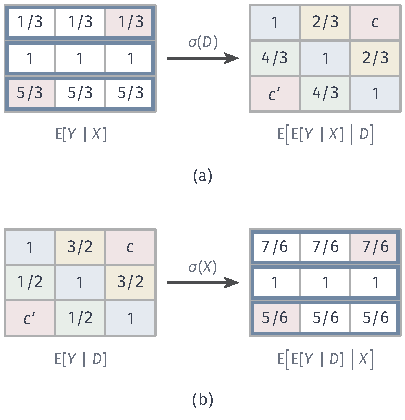
\includegraphics[width=68mm]{figures/07-probability/02-measure-theoretic-probability/tikz/cexp-tower-non-nested/figure.pdf}
  \caption{互不包含的两份信息，传感器表。蓝框表示按行（$\sigma(X)$）取常数，同色格子表示按对角线（$\sigma(D)$，$D=X-Y$）取常数，$c$、$c'$是零概率组上的任意常数。(a)先给定$X$再给定$D$。(b)先给定$D$再给定$X$。两个结果不同，也都不是常数$\mathbb{E}[Y]=1$。}
  \label{fig:cexp-tower-non-nested}
\end{BookInlineFigure}

两种顺序的结果一个是$D$的函数，一个是$X$的函数，彼此不同。它们也都不等于在共同信息$\sigma(X)\cap\sigma(D)$上的平均：一个事件若同时是若干整行之并和若干整条对角线之并，只要含有某一行，就含有这一行经过的对角线，进而含有那些对角线经过的其他行，最后只能是$\Omega$；所以共同信息只有$\{\emptyset,\Omega\}$，相应的平均是常数$1$。两份信息各自有用，交起来却什么也不剩，先后两次平均在两种顺序下也都没有抵达这个常数。


\section{条件期望的不等式}
\label{sec:cexp-inequalities}

条件期望对线性运算可以逐项进行，对非线性运算却不行：$\mathbb{E}[Y^{2}\mid X]$与$(\mathbb{E}[Y\mid X])^{2}$一般不相等。传感器表的第二行中，前者是$3/2$，后者是$1$。“先在组内平均再平方”与“先平方再在组内平均”之间的差别有确定的方向吗？第~\ref{chap:random-variable-moments}章用凸函数回答了不带条件的情形，这一节把它推广到给定信息的情形，再把绝对值的幂作为特例，得到条件期望对$L^{p}$大小的控制。

\subsection{条件Jensen不等式}
\label{sec:cexp-jensen}

\paragraph{可数条支撑线}
第~\ref{chap:random-variable-moments}章的Jensen不等式在$\mathbb{E}[X]$这一点放一条支撑线，再对两边取期望。给定信息时，条件平均$\mathbb{E}[X\mid\mathcal{G}]$随样本点变化，支撑点也随之变化，需要同时用到许多条支撑线。每条支撑线给出的不等式都只在一个零概率集之外成立，为了能把例外集并起来，支撑线只能取可数多条。下面的引理说明可数条已经足够。

\begin{lemma}[凸函数是可数条直线的上包络]
\label{lem:cexp-countable-lines}
设$\varphi:\mathbb{R}\to\mathbb{R}$是凸函数。对每个有理数$q$，取$\varphi$在$q$处的一条支撑线的斜率$s_q$，即$\varphi(x)\geq\varphi(q)+s_q(x-q)$对一切$x$成立。则对每个实数$x$，
\begin{equation}
 \varphi(x)=\sup_{q\in\mathbb{Q}}\bigl(\varphi(q)+s_q(x-q)\bigr).
 \label{eq:cexp-countable-lines}
\end{equation}
\end{lemma}

\begin{proof}
支撑线的存在见第~\ref{chap:random-variable-moments}章。由支撑线的定义，右边不超过$\varphi(x)$，只需说明右边能任意接近$\varphi(x)$。

先说明靠近$x$的支撑点上，斜率有统一的界。凸函数在$\mathbb{R}$上连续，设$\lvert\varphi\rvert$在$[x-2,x+2]$上不超过$M$。对$q\in[x-1,x+1]$，把支撑线不等式用在$x+2$处，移项得
\[
 s_q\leq\frac{\varphi(x+2)-\varphi(q)}{x+2-q}\leq\frac{2M}{1}=2M ,
\]
这里用了$x+2-q\geq1$。同样把它用在$x-2$处，得$s_q\geq-2M$。所以$\lvert s_q\rvert\leq2M$。

于是对$q\in[x-1,x+1]\cap\mathbb{Q}$，
\[
 \varphi(q)+s_q(x-q)\geq\varphi(q)-2M\lvert x-q\rvert .
\]
令有理数$q\to x$，由$\varphi$的连续性，右边趋于$\varphi(x)$。
\end{proof}

\paragraph{不等式与证明}
有了可数条支撑线，对每一条用一次条件期望的线性与保序，再取上确界。

\begin{theorem}[条件Jensen不等式]
\label{thm:cexp-jensen}
设$\varphi:\mathbb{R}\to\mathbb{R}$是凸函数，$X$与$\varphi(X)$都可积。则
\begin{equation}
 \varphi\bigl(\mathbb{E}[X\mid\mathcal{G}]\bigr)\leq\mathbb{E}\bigl[\varphi(X)\bigm|\mathcal{G}\bigr].
 \label{eq:cexp-jensen}
\end{equation}
\end{theorem}

\begin{proof}
记$Z=\mathbb{E}[X\mid\mathcal{G}]$。对每个有理数$q$，由支撑线不等式，
\[
 \varphi(X)\geq\varphi(q)+s_q(X-q)
\]
处处成立。两边都可积，由定理~\ref{thm:cexp-linearity}的保序与线性，存在零概率事件$N_q$，在$N_q$之外
\[
 \mathbb{E}\bigl[\varphi(X)\bigm|\mathcal{G}\bigr]\geq\varphi(q)+s_q(Z-q).
\]
令$N=\bigcup_{q\in\mathbb{Q}}N_q$，它是可数个零概率事件之并，概率仍为零。在$N$之外，上式对所有有理数$q$同时成立，对$q$取上确界，由式~\eqref{eq:cexp-countable-lines}，右边成为$\varphi(Z)$。
\end{proof}

式~\eqref{eq:cexp-jensen}称为\term{条件Jensen不等式}（conditional Jensen inequality）。定理的条件各有作用。凸性决定方向：组内平均把点拉向组内的重心，凸函数在重心处的值不超过函数值的平均。$X$与$\varphi(X)$可积，保证两边的条件期望都有定义。可数性藏在证明里：如果直接对每个实数$q$使用支撑线，会得到不可数多个例外集，它们的并可能不是零概率集。

\paragraph{用平方函数检验方向}
取$\varphi(y)=y^{2}$。设$X$平方可积，式~\eqref{eq:cexp-jensen}给出
\[
 \bigl(\mathbb{E}[X\mid\mathcal{G}]\bigr)^{2}\leq\mathbb{E}[X^{2}\mid\mathcal{G}] .
\]
传感器表三行的两边依次是
\[
 \tfrac19\leq\tfrac13,\qquad 1\leq\tfrac32,\qquad \tfrac{25}{9}\leq3 ,
\]
差值$2/9$、$1/2$、$2/9$正是第~\ref{chap:random-vectors}章算出的三行条件方差，第~\ref{sec:cexp-conditional-variance}节会在一般情形下定义它。图~\ref{fig:cexp-jensen}(a)画出第二行的几何：三个点$(y,y^{2})$按条件概率$\tfrac14,\tfrac12,\tfrac14$加权，重心的高度是$3/2$，高于抛物线在重心横坐标$1$处的高度$1$；紫色虚线是$y=1$处的支撑线。

\begin{BookInlineFigure}
  \centering
  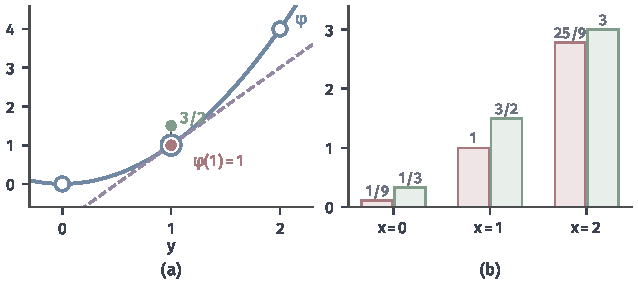
\includegraphics[width=108mm]{figures/07-probability/02-measure-theoretic-probability/matplotlib/cexp-jensen/figure.pdf}
  \caption{条件Jensen不等式，$\varphi(y)=y^{2}$，传感器表。(a)第二行$X=1$：空心圆是$(y,y^{2})$，大小与条件概率$\tfrac14,\tfrac12,\tfrac14$成正比；红点是$\varphi(\mathbb{E}[Y\mid X=1])=1$，绿点是$\mathbb{E}[Y^{2}\mid X=1]=3/2$，紫色虚线是$y=1$处的支撑线。(b)三行的$(\mathbb{E}[Y\mid X=x])^{2}$（红）与$\mathbb{E}[Y^{2}\mid X=x]$（绿）。}
  \label{fig:cexp-jensen}
\end{BookInlineFigure}

若$\varphi$是凹函数，对$-\varphi$用定理，不等号反向。例如对凹函数$-y^{2}$，得到的不等式两边乘以$-1$后就是上面的平方不等式。既不凸也不凹的函数没有确定的方向。取$\varphi(y)=y^{3}$，它在$[0,\infty)$上凸，在$(-\infty,0]$上凹。传感器表第一行中$Y$以$\tfrac23,\tfrac13$取$0,1$，两个值落在凸段上，
\[
 \bigl(\mathbb{E}[Y\mid X=0]\bigr)^{3}=\tfrac{1}{27}<\tfrac13=\mathbb{E}[Y^{3}\mid X=0].
\]
把变量平移成$Y-2$，第一行的两个值$-2,-1$落在凹段上，方向随之反转：
\[
 \bigl(\mathbb{E}[Y-2\mid X=0]\bigr)^{3}=-\tfrac{125}{27}\approx-4.63>-\tfrac{17}{3}\approx-5.67=\mathbb{E}\bigl[(Y-2)^{3}\bigm|X=0\bigr].
\]
同一个函数，作用在落于不同区段的取值上，可以给出相反的方向；只有在整个$\mathbb{R}$上凸，才能对一切变量和一切信息保证式~\eqref{eq:cexp-jensen}。

\subsection{\texorpdfstring{$L^p$}{Lp}收缩}
\label{sec:cexp-lp}

\paragraph{条件平均不放大\texorpdfstring{$L^{p}$}{Lp}范数}
对$1\leq p<\infty$，记
\[
 \lVert X\rVert_p=\bigl(\mathbb{E}\lvert X\rvert^{p}\bigr)^{1/p},
\]
$L^{p}$是满足$\lVert X\rVert_p<\infty$的随机变量组成的空间，两个几乎必然相等的随机变量视为同一个元素，见\BookChapterRef{chap:function-normed-spaces}{卷四第11章“赋范空间”}。在概率空间上，$L^{p}\subseteq L^{1}$：由逐点的不等式$\lvert x\rvert\leq1+\lvert x\rvert^{p}$取期望，得到$X$可积。再对凸函数$y\mapsto\lvert y\rvert^{p}$和可积的$\lvert X\rvert$用第~\ref{chap:random-variable-moments}章的Jensen不等式，
\[
 \bigl(\mathbb{E}\lvert X\rvert\bigr)^{p}\leq\mathbb{E}\lvert X\rvert^{p},
\]
即$\lVert X\rVert_1\leq\lVert X\rVert_p$。所以$L^{p}$中的随机变量都有条件期望。把条件Jensen不等式用于$\varphi(y)=\lvert y\rvert^{p}$，就得到条件期望对$L^{p}$范数的控制。

\begin{theorem}[\texorpdfstring{$L^{p}$}{Lp}收缩]
\label{thm:cexp-lp}
设$1\leq p<\infty$，$X\in L^{p}$。则$\mathbb{E}[X\mid\mathcal{G}]\in L^{p}$，并且
\begin{equation}
 \bigl\lVert\mathbb{E}[X\mid\mathcal{G}]\bigr\rVert_p\leq\lVert X\rVert_p .
 \label{eq:cexp-lp}
\end{equation}
\end{theorem}

\begin{proof}
$\varphi(y)=\lvert y\rvert^{p}$是$\mathbb{R}$上的凸函数，$X$与$\lvert X\rvert^{p}$都可积。由条件Jensen不等式，
\[
 \bigl\lvert\mathbb{E}[X\mid\mathcal{G}]\bigr\rvert^{p}\leq\mathbb{E}\bigl[\lvert X\rvert^{p}\bigm|\mathcal{G}\bigr].
\]
两边非负，取期望，右边由全期望公式等于$\mathbb{E}\lvert X\rvert^{p}$，于是
\[
 \mathbb{E}\bigl\lvert\mathbb{E}[X\mid\mathcal{G}]\bigr\rvert^{p}\leq\mathbb{E}\lvert X\rvert^{p}<\infty .
\]
两边开$p$次方即得。
\end{proof}

$p=\infty$的情形更直接：若$\lvert X\rvert\leq c$几乎必然成立，由保序，$\lvert\mathbb{E}[X\mid\mathcal{G}]\rvert\leq c$几乎必然成立。

\paragraph{对扰动的稳定性}
把定理用于两个输入之差。设$X_1,X_2\in L^{p}$，由线性，
\begin{equation}
 \bigl\lVert\mathbb{E}[X_1\mid\mathcal{G}]-\mathbb{E}[X_2\mid\mathcal{G}]\bigr\rVert_p\leq\lVert X_1-X_2\rVert_p .
 \label{eq:cexp-lp-stability}
\end{equation}
条件期望是$L^{p}$上的线性映射，范数不超过$1$：输入有一点扰动，输出的扰动不会更大。由此，若$X_n\to X$在$L^{p}$中成立，则$X_n$的条件期望也在$L^{p}$中收敛到$\mathbb{E}[X\mid\mathcal{G}]$，条件期望与$L^{p}$极限可以交换次序。

\paragraph{逐次等分的数值}
用逐次等分的例子观察这个不等式，把$X$中心化，取$X(\omega)=\omega^{2}-\tfrac13$。$n=1$时，两段上的平均是$\tfrac1{12}-\tfrac13$与$\tfrac{7}{12}-\tfrac13$，即
\[
 \mathbb{E}[X\mid\mathcal{G}_1]=-\tfrac14\ \text{在}\ [0,\tfrac12)\ \text{上},\qquad
 \mathbb{E}[X\mid\mathcal{G}_1]=\tfrac14\ \text{在}\ [\tfrac12,1)\ \text{上}.
\]
$\lvert\mathbb{E}[X\mid\mathcal{G}_1]\rvert$恒为$1/4$，所以它的各阶范数都是$1/4$。另一方面，$X$在$\omega_0=1/\sqrt3$处变号，分两段积分，
\[
 \lVert X\rVert_1=\int_0^{\omega_0}\Bigl(\frac13-\omega^{2}\Bigr)\mathrm{d}\omega+\int_{\omega_0}^{1}\Bigl(\omega^{2}-\frac13\Bigr)\mathrm{d}\omega=\frac{4}{9\sqrt3}\approx0.2566 .
\]
$\lVert X\rVert_2^{2}$是$\omega^{2}$的方差$\tfrac15-\tfrac19=\tfrac4{45}$，所以$\lVert X\rVert_2\approx0.2981$。两者都大于$1/4$，与式~\eqref{eq:cexp-lp}一致。

图~\ref{fig:cexp-lp-contraction}(a)画出$n=0,1,\dots,7$时$\lVert\mathbb{E}[X\mid\mathcal{G}_n]\rVert_p$，三条绿色折线分别对应$p=1,2,4$，都停在紫色虚线$\lVert X\rVert_p$之下。折线随$n$不减，这可以由塔式法则解释：$\mathcal{G}_n\subseteq\mathcal{G}_{n+1}$，由式~\eqref{eq:cexp-tower}，
\[
 \mathbb{E}[X\mid\mathcal{G}_n]=\mathbb{E}\bigl[\mathbb{E}[X\mid\mathcal{G}_{n+1}]\bigm|\mathcal{G}_n\bigr],
\]
把$\mathbb{E}[X\mid\mathcal{G}_{n+1}]$当作输入，对右边用式~\eqref{eq:cexp-lp}，得到
\[
 \bigl\lVert\mathbb{E}[X\mid\mathcal{G}_n]\bigr\rVert_p\leq\bigl\lVert\mathbb{E}[X\mid\mathcal{G}_{n+1}]\bigr\rVert_p .
\]
图中各折线还逐渐贴近上界。信息逐步增加时条件期望的收敛属于鞅的理论，可参考\BookChapterRef{chap:discrete-time-stochastic-processes}{卷九第3章“离散时间随机过程”}；这里只把它作为数值观察。

\begin{BookInlineFigure}
  \centering
  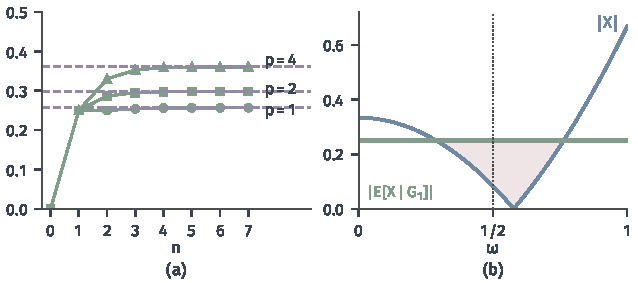
\includegraphics[width=108mm]{figures/07-probability/02-measure-theoretic-probability/matplotlib/cexp-lp-contraction/figure.pdf}
  \caption{$L^{p}$收缩，$\Omega=[0,1)$，$X(\omega)=\omega^{2}-\tfrac13$，$\mathcal{G}_n$由$2^{n}$个等长区间生成，范数用$2^{16}$个小区间上的中点公式计算。(a)$\lVert\mathbb{E}[X\mid\mathcal{G}_n]\rVert_p$（绿；圆、方、三角分别对应$p=1,2,4$）与$\lVert X\rVert_p$（紫色虚线）。(b)$n=1$时的$\lvert X\rvert$（蓝）与$\lvert\mathbb{E}[X\mid\mathcal{G}_1]\rvert$（绿），浅红区域上后者更大。}
  \label{fig:cexp-lp-contraction}
\end{BookInlineFigure}

\paragraph{控制的是总体大小}
式~\eqref{eq:cexp-lp}控制的是范数，即对整个$\Omega$平均后的大小，不是逐点的大小。图~\ref{fig:cexp-lp-contraction}(b)中，$\omega$在$\omega_0\approx0.577$附近时$\lvert X\rvert$接近$0$，而$\lvert\mathbb{E}[X\mid\mathcal{G}_1]\rvert=1/4$，浅红区域上条件平均的绝对值比原变量大。组内平均把组内的值拉向同一个数，原来接近零的样本点被拉离零，原来远离零的被拉近；拉近的部分在范数中占上风。传感器表中同样如此：格子$(0,0)$上$Y=0$，$\mathbb{E}[Y\mid X]=1/3$。


\section{最小均方预测}
\label{sec:cexp-prediction}

到目前为止，条件期望只被描述为“保留累计期望的组内平均”。它还有一个优化的含义：如果只能根据已知信息去猜$X$，并以平方误差的平均衡量猜得好坏，最好的猜法就是条件期望。第~\ref{chap:random-vectors}章在形如$a+bx$的直线中找过最好的预测，这里不限定形式，允许使用已知信息的任意函数，只要求预测量平方可积。

设$X$平方可积。一个只用$\mathcal{G}$中信息的预测量是一个$\mathcal{G}$可测的随机变量$W$，要求$\mathbb{E}[W^{2}]<\infty$；它的\term{均方误差}（mean squared error）是$\mathbb{E}[(X-W)^{2}]$。问题是：在所有这样的$W$中，哪一个使均方误差最小？卷四的Hilbert空间投影给出了现成的框架。

\subsection{正交投影}
\label{sec:cexp-projection}

\paragraph{预测量组成的子空间}
平方可积随机变量组成$L^{2}=L^{2}(\Omega,\mathcal{F},\mathbb{P})$，内积为$\langle U,V\rangle=\mathbb{E}[UV]$，范数为$\lVert U\rVert_2=(\mathbb{E}[U^{2}])^{1/2}$。卷四证明了$L^{2}$是Hilbert空间，并且对Hilbert空间的闭线性子空间$M$与任一元素$f$，$M$中离$f$最近的元素存在且唯一，它由“$f$减去它与$M$正交”刻画，可参考\BookChapterRef{chap:function-inner-product-spaces}{卷四第12章“内积空间”}。

记
\[
 L^{2}(\mathcal{G})=\bigl\{W\in L^{2}:\ W\ \text{几乎必然等于某个}\ \mathcal{G}\ \text{可测的随机变量}\bigr\}.
\]
它是全体候选预测量。均方误差$\mathbb{E}[(X-W)^{2}]$就是$\lVert X-W\rVert_2^{2}$，所以最小均方预测是在$L^{2}(\mathcal{G})$中找离$X$最近的点。要用投影定理，先确认这个集合是闭线性子空间。

\begin{lemma}[已知信息上的平方可积变量]
\label{lem:cexp-closed-subspace}
$L^{2}(\mathcal{G})$是$L^{2}$的闭线性子空间。
\end{lemma}

\begin{proof}
$\mathcal{G}$可测的函数的线性组合仍$\mathcal{G}$可测，所以$L^{2}(\mathcal{G})$是线性子空间。

闭性借助完备性。$L^{2}(\mathcal{G})$中的元素与概率空间$(\Omega,\mathcal{G},\mathbb{P}_{\mathcal{G}})$上的平方可积函数一一对应，并且对$\mathcal{G}$可测的函数，对$\mathbb{P}_{\mathcal{G}}$与对$\mathbb{P}$的积分相同（见定理~\ref{thm:cexp-existence}的证明），所以这一对应保持范数。$L^{2}(\Omega,\mathcal{G},\mathbb{P}_{\mathcal{G}})$本身是Hilbert空间，因而完备。设$W_n\in L^{2}(\mathcal{G})$在$L^{2}$中收敛到$W$，则$(W_n)$是Cauchy列，在$L^{2}(\Omega,\mathcal{G},\mathbb{P}_{\mathcal{G}})$中收敛到某个$\mathcal{G}$可测的$W'$，也就在$L^{2}$中收敛到$W'$。极限唯一，$W=W'$几乎必然成立，所以$W\in L^{2}(\mathcal{G})$。
\end{proof}

这里不能简单地说“$\mathcal{G}$可测函数的极限仍$\mathcal{G}$可测”：$L^{2}$收敛只给出一个子列几乎必然收敛，而例外的零概率集未必属于$\mathcal{G}$。借助完备性绕开了这个问题。

\paragraph{残差与已知信息正交}
现在说明条件期望正是投影。思路是：把式~\eqref{eq:cexp-defining}中的示性函数$\mathbf{1}_{A}$换成一般的$W\in L^{2}(\mathcal{G})$。

\begin{theorem}[条件期望是正交投影]
\label{thm:cexp-projection}
设$X\in L^{2}$。则$\mathbb{E}[X\mid\mathcal{G}]\in L^{2}(\mathcal{G})$，并且对每个$W\in L^{2}(\mathcal{G})$，
\begin{equation}
 \mathbb{E}\bigl[(X-\mathbb{E}[X\mid\mathcal{G}])\,W\bigr]=0 .
 \label{eq:cexp-orthogonality}
\end{equation}
因此$\mathbb{E}[X\mid\mathcal{G}]$是$X$在$L^{2}(\mathcal{G})$上的正交投影。
\end{theorem}

\begin{proof}
记$Z=\mathbb{E}[X\mid\mathcal{G}]$。由定理~\ref{thm:cexp-lp}取$p=2$，$Z\in L^{2}$，它又是$\mathcal{G}$可测的，所以$Z\in L^{2}(\mathcal{G})$。

取$W\in L^{2}(\mathcal{G})$，不妨设$W$本身$\mathcal{G}$可测。由Cauchy--Schwarz不等式，
\[
 \mathbb{E}\lvert WX\rvert\leq\lVert W\rVert_2\lVert X\rVert_2<\infty ,
\]
所以$WX$可积。由提取已知量，$\mathbb{E}[WX\mid\mathcal{G}]=WZ$；两边取期望，由全期望公式，
\[
 \mathbb{E}[WX]=\mathbb{E}\bigl[\mathbb{E}[WX\mid\mathcal{G}]\bigr]=\mathbb{E}[WZ] .
\]
移项即得式~\eqref{eq:cexp-orthogonality}。$X-Z$与闭子空间$L^{2}(\mathcal{G})$正交，而$Z$在这个子空间中，由卷四的正交刻画，$Z$是$X$在其上的正交投影。
\end{proof}

正交条件~\eqref{eq:cexp-orthogonality}是积分刻画的推广。取$W=\mathbf{1}_{A}$，$A\in\mathcal{G}$，它就是式~\eqref{eq:cexp-defining}：残差$X-Z$在每个已知事件上的累计为零。反过来，若某个$Z\in L^{2}(\mathcal{G})$满足正交条件，取$W=\mathbf{1}_{A}$就知道它满足条件期望的定义。所以对平方可积的$X$，投影定理本身就给出了条件期望的存在性，不必经过Radon--Nikodym定理。这条路线只覆盖平方可积的情形；对只可积的$X$，存在性仍由定理~\ref{thm:cexp-existence}保证。

\paragraph{传感器表中的投影}
传感器表把这幅几何图景变成了有限维的计算。七个正概率格子上的函数组成一个七维空间，内积是按格子概率加权的乘积和。$\sigma(X)$可测的函数是在每行取常数的函数，组成一个三维子空间。$Y$在它上面的投影就是按行平均，残差$Y-\mathbb{E}[Y\mid X]$在每行内的加权和为零，因而与每一个行常数函数正交。

勾股定理给出平方长度的拆分。记$m(X)=\mathbb{E}[Y\mid X]$，第~\ref{chap:random-vectors}章已算得$\operatorname{Var}(Y)=0.6$、$\operatorname{Var}(m(X))=4/15$、平均条件方差为$1/3$，于是
\[
 \mathbb{E}[Y^{2}]=1.6,\qquad \mathbb{E}\bigl[m(X)^{2}\bigr]=\tfrac{4}{15}+1=\tfrac{19}{15},\qquad \mathbb{E}\bigl[(Y-m(X))^{2}\bigr]=\tfrac13 ,
\]
并且$\tfrac{19}{15}+\tfrac{5}{15}=\tfrac{24}{15}=1.6$。图~\ref{fig:cexp-projection}是这一关系的示意：$X$到平面$L^{2}(\mathcal{G})$的垂线足是$\mathbb{E}[X\mid\mathcal{G}]$。

\begin{BookInlineFigure}
  \centering
  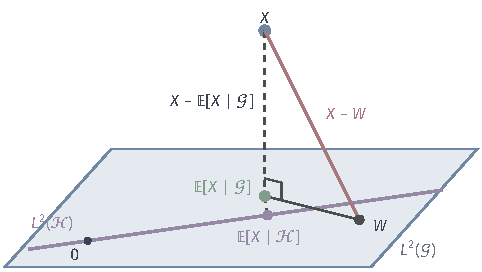
\includegraphics[width=82mm]{figures/07-probability/02-measure-theoretic-probability/tikz/cexp-projection/figure.pdf}
  \caption{条件期望是正交投影（示意）。浅蓝平面是$L^{2}(\mathcal{G})$，平面内的紫线是较小信息$\mathcal{H}\subseteq\mathcal{G}$对应的$L^{2}(\mathcal{H})$，常数（含$0$）都在其中。$X$的垂线足是$\mathbb{E}[X\mid\mathcal{G}]$（绿），残差（虚线）与平面垂直；平面中另一点$W$与$X$的距离（红）更长。再把$\mathbb{E}[X\mid\mathcal{G}]$投影到紫线上，得到$\mathbb{E}[X\mid\mathcal{H}]$。}
  \label{fig:cexp-projection}
\end{BookInlineFigure}

投影的观点也解释了塔式法则。$\mathcal{H}\subseteq\mathcal{G}$时$L^{2}(\mathcal{H})\subseteq L^{2}(\mathcal{G})$，先投影到大的子空间再投影到小的子空间，等于直接投影到小的子空间；先投影到小的子空间，结果已在大的子空间中，再投影到大的子空间不改变它。这正是式~\eqref{eq:cexp-tower}的两个等号在平方可积情形的几何含义。

\subsection{平方误差分解}
\label{sec:cexp-mse}

\paragraph{误差的勾股定理}
正交性直接给出任一预测量的误差构成。

\begin{theorem}[平方误差分解]
\label{thm:cexp-mse}
设$X\in L^{2}$，$Z=\mathbb{E}[X\mid\mathcal{G}]$。对每个$W\in L^{2}(\mathcal{G})$，
\begin{equation}
 \mathbb{E}\bigl[(X-W)^{2}\bigr]=\mathbb{E}\bigl[(X-Z)^{2}\bigr]+\mathbb{E}\bigl[(Z-W)^{2}\bigr].
 \label{eq:cexp-mse}
\end{equation}
因此$Z$在$L^{2}(\mathcal{G})$中使均方误差最小，并且使均方误差最小的$W$几乎必然等于$Z$。
\end{theorem}

\begin{proof}
把预测误差拆成两段：
\[
 X-W=(X-Z)+(Z-W).
\]
平方后取期望，交叉项是$2\,\mathbb{E}[(X-Z)(Z-W)]$。$Z-W\in L^{2}(\mathcal{G})$，由式~\eqref{eq:cexp-orthogonality}，交叉项为零，得到式~\eqref{eq:cexp-mse}。右边第二项非负，所以$\mathbb{E}[(X-W)^{2}]\geq\mathbb{E}[(X-Z)^{2}]$；等号成立当且仅当$\mathbb{E}[(Z-W)^{2}]=0$，即$W=Z$几乎必然成立。
\end{proof}

式~\eqref{eq:cexp-mse}把误差分成两部分：$\mathbb{E}[(X-Z)^{2}]$是已知信息无论如何也消除不了的部分，与$W$无关；$\mathbb{E}[(Z-W)^{2}]$是$W$偏离最佳预测而多付的代价。

用传感器表演示。取$\mathcal{G}=\sigma(X)$，再取一个较差的预测$W=\mathbb{E}[Y\mid\mathcal{H}]$，$\mathcal{H}=\sigma(\mathbf{1}_{\{X=2\}})$。它在前两行取$5/7$、第三行取$5/3$，是行常数函数，属于$L^{2}(\sigma(X))$。按行计算多付的代价：
\[
 \mathbb{E}\bigl[(Z-W)^{2}\bigr]=0.3\Bigl(\frac13-\frac57\Bigr)^{2}+0.4\Bigl(1-\frac57\Bigr)^{2}+0.3\cdot0=\frac{64}{1470}+\frac{16}{490}=\frac{8}{105}.
\]
再加上不可消除的部分$1/3$，
\[
 \mathbb{E}\bigl[(Y-W)^{2}\bigr]=\frac13+\frac{8}{105}=\frac{43}{105}\approx0.410 .
\]
直接按格子计算$(Y-W)^{2}$的加权和，也得到$43/105$。

\paragraph{信息多了，误差平均不增}
若$\mathcal{H}\subseteq\mathcal{G}$，则$\mathbb{E}[X\mid\mathcal{H}]\in L^{2}(\mathcal{H})\subseteq L^{2}(\mathcal{G})$，可以取它作为式~\eqref{eq:cexp-mse}中的$W$，得到
\begin{equation}
 \mathbb{E}\bigl[(X-\mathbb{E}[X\mid\mathcal{H}])^{2}\bigr]=\mathbb{E}\bigl[(X-\mathbb{E}[X\mid\mathcal{G}])^{2}\bigr]+\mathbb{E}\bigl[(\mathbb{E}[X\mid\mathcal{G}]-\mathbb{E}[X\mid\mathcal{H}])^{2}\bigr].
 \label{eq:cexp-information-monotone}
\end{equation}
更多的信息使最小均方误差不增，减少的量恰好是两个最佳预测之差的平方平均。上面的数值正是这一式的例子：只知道“是否偏高”时最小误差是$43/105$，知道完整的第一台读数后降到$1/3$。

这只是平均意义下的结论，不是逐个样本点的结论。图~\ref{fig:cexp-pointwise-error}比较七个正概率格子上的平方误差。格子$(0,1)$上$Y=1$，较粗的预测$5/7$误差为$4/49\approx0.08$，较细的预测$1/3$误差为$4/9\approx0.44$；格子$(1,0)$上误差也从约$0.51$增到$1$。信息变多后，这两个格子的预测变差了；但其他格子的改善更多，按概率加权后总体误差从$0.410$降到$0.333$。

\begin{BookInlineFigure}
  \centering
  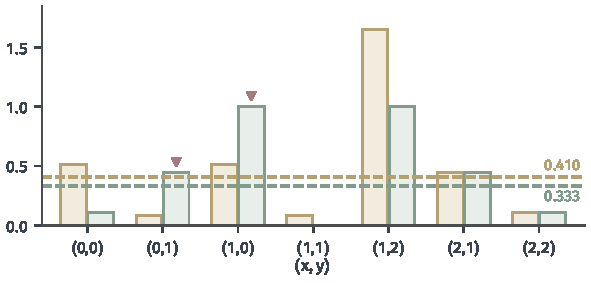
\includegraphics[width=100mm]{figures/07-probability/02-measure-theoretic-probability/matplotlib/cexp-pointwise-error/figure.pdf}
  \caption{逐格的平方误差，传感器表的七个正概率格子。黄柱：用$\mathbb{E}[Y\mid\mathcal{H}]$预测，$\mathcal{H}=\sigma(\mathbf{1}_{\{X=2\}})$；绿柱：用$\mathbb{E}[Y\mid X]$预测。红色三角标出信息增加后误差变大的格子$(0,1)$与$(1,0)$；两条虚线是按概率加权的平均误差$43/105\approx0.410$与$1/3$。}
  \label{fig:cexp-pointwise-error}
\end{BookInlineFigure}

最小化是在所有$\mathcal{G}$可测的平方可积预测量中进行的，不限于线性函数。传感器表与三角形模型中，$\mathbb{E}[Y\mid X]$恰好是$X$的线性函数，所以第~\ref{chap:random-vectors}章的最佳直线与这里的最佳预测重合。“只知绝对值”的例子中，$\mathrm{e}^{X}$的最佳预测$\cosh\lvert X\rvert$不是$\lvert X\rvert$的线性函数，最佳直线的均方误差就严格大于最佳预测的均方误差。从样本中估计这样的预测函数是统计推断的问题，可参考\BookChapterRef{chap:nonparametric-inference}{卷八第2章“非参数分布与函数推断”}。

\subsection{条件方差与全方差公式}
\label{sec:cexp-conditional-variance}

\paragraph{条件方差}
最小误差$\mathbb{E}[(X-Z)^{2}]$是一个数，它是对整个$\Omega$平均的结果。在每个已知群体内，残差平方的平均可以不同：传感器表中，第一行与第三行的条件方差是$2/9$，第二行是$1/2$。把残差平方再给定$\mathcal{G}$求条件期望，就得到随已知信息变化的波动大小。

\begin{definition}[条件方差]
\label{def:cexp-conditional-variance}
设$X\in L^{2}$，$Z=\mathbb{E}[X\mid\mathcal{G}]$。称
\begin{equation}
 \operatorname{Var}(X\mid\mathcal{G})=\mathbb{E}\bigl[(X-Z)^{2}\bigm|\mathcal{G}\bigr]
 \label{eq:cexp-conditional-variance}
\end{equation}
为$X$给定$\mathcal{G}$的条件方差。给定随机对象$Y$时取$\mathcal{G}=\sigma(Y)$，记作$\operatorname{Var}(X\mid Y)$。
\end{definition}

$(X-Z)^{2}$可积，因为$X,Z\in L^{2}$，所以定义有意义。它是$\mathcal{G}$可测的非负随机变量，只确定到零概率集。给定离散或有密度的$Y$时，第~\ref{chap:random-vectors}章的$v(y)=\operatorname{Var}(X\mid Y=y)$经过复合得到它的一个版本，理由与第~\ref{sec:cexp-given-variable}节的条件均值相同。

与不带条件的方差一样，条件方差有二阶矩的写法：
\begin{equation}
 \operatorname{Var}(X\mid\mathcal{G})=\mathbb{E}[X^{2}\mid\mathcal{G}]-\bigl(\mathbb{E}[X\mid\mathcal{G}]\bigr)^{2}.
 \label{eq:cexp-conditional-variance-moment}
\end{equation}
推导时把平方展开，$(X-Z)^{2}=X^{2}-2XZ+Z^{2}$，三项都可积，其中$XZ$的可积性由Cauchy--Schwarz不等式保证。对三项分别求条件期望，$Z$是已知量，由提取已知量，
\[
 \mathbb{E}[XZ\mid\mathcal{G}]=Z\,\mathbb{E}[X\mid\mathcal{G}]=Z^{2},\qquad \mathbb{E}[Z^{2}\mid\mathcal{G}]=Z^{2}.
\]
再由线性，
\[
 \operatorname{Var}(X\mid\mathcal{G})=\mathbb{E}[X^{2}\mid\mathcal{G}]-2Z^{2}+Z^{2}=\mathbb{E}[X^{2}\mid\mathcal{G}]-Z^{2}.
\]
由条件Jensen不等式，右边几乎必然非负，与定义一致。传感器表中，由第~\ref{sec:cexp-known}节的$\mathbb{E}[Y^{2}\mid X]$，第二行为$\tfrac32-1^{2}=\tfrac12$。

\needspace{8\baselineskip}
\paragraph{全方差公式}
有了条件方差，总方差可以拆成两部分。

\begin{theorem}[全方差公式]
\label{thm:cexp-total-variance}
设$X\in L^{2}$。则
\begin{equation}
 \operatorname{Var}(X)=\mathbb{E}\bigl[\operatorname{Var}(X\mid\mathcal{G})\bigr]+\operatorname{Var}\bigl(\mathbb{E}[X\mid\mathcal{G}]\bigr).
 \label{eq:cexp-total-variance}
\end{equation}
\end{theorem}

\begin{proof}
记$Z=\mathbb{E}[X\mid\mathcal{G}]$。常数$\mathbb{E}[X]$属于$L^{2}(\mathcal{G})$，在式~\eqref{eq:cexp-mse}中取$W=\mathbb{E}[X]$，
\[
 \mathbb{E}\bigl[(X-\mathbb{E}[X])^{2}\bigr]=\mathbb{E}\bigl[(X-Z)^{2}\bigr]+\mathbb{E}\bigl[(Z-\mathbb{E}[X])^{2}\bigr].
\]
左边是$\operatorname{Var}(X)$。右边第一项由全期望公式与式~\eqref{eq:cexp-conditional-variance}，
\[
 \mathbb{E}\bigl[(X-Z)^{2}\bigr]=\mathbb{E}\Bigl[\mathbb{E}\bigl[(X-Z)^{2}\bigm|\mathcal{G}\bigr]\Bigr]=\mathbb{E}\bigl[\operatorname{Var}(X\mid\mathcal{G})\bigr].
\]
由全期望公式$\mathbb{E}[Z]=\mathbb{E}[X]$，所以第二项是$\operatorname{Var}(Z)$。
\end{proof}

第一项是组内波动的平均，第二项是各组平均之间的波动。第~\ref{chap:random-vectors}章对概率表和联合密度分别证明过这个公式，现在它对任何信息都成立，证明只用到正交分解。

\paragraph{信息怎样重新分配方差}
总方差是固定的，信息只是在两项之间重新分配。图~\ref{fig:cexp-information-variance}(a)对传感器表的四层信息
\[
 \{\emptyset,\Omega\}\subseteq\mathcal{H}\subseteq\sigma(X)\subseteq\sigma(X,Y)
\]
画出这一分配。什么也不知道时，全部$0.6$都是组内波动；知道“是否偏高”时拆成$\tfrac{43}{105}+\tfrac{4}{21}$；知道第一台读数时拆成$\tfrac13+\tfrac{4}{15}$；知道两台读数时$Y$已知，全部是组间波动。由式~\eqref{eq:cexp-information-monotone}，组内波动的平均随信息增加而不增。$\mathcal{H}$这一层的组间部分可以直接算：$\mathbb{E}[Y\mid\mathcal{H}]$以概率$0.7,0.3$取$5/7,5/3$，均值为$1$，
\[
 \operatorname{Var}\bigl(\mathbb{E}[Y\mid\mathcal{H}]\bigr)=0.7\Bigl(\frac57-1\Bigr)^{2}+0.3\Bigl(\frac53-1\Bigr)^{2}=\frac{2}{35}+\frac{2}{15}=\frac{4}{21}.
\]

\begin{BookInlineFigure}
  \centering
  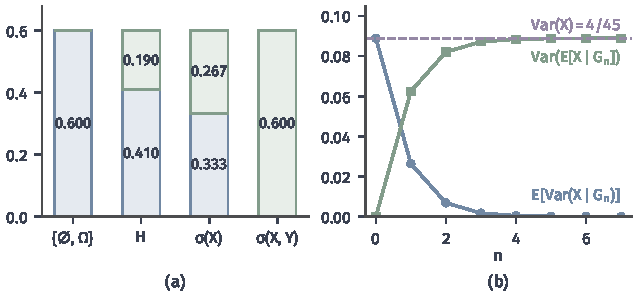
\includegraphics[width=108mm]{figures/07-probability/02-measure-theoretic-probability/matplotlib/cexp-information-variance/figure.pdf}
  \caption{全方差公式在信息增加时的分配。浅蓝或蓝色表示$\mathbb{E}[\operatorname{Var}(\cdot\mid\mathcal{G})]$，浅绿或绿色表示$\operatorname{Var}(\mathbb{E}[\cdot\mid\mathcal{G}])$。(a)传感器表中$Y$的方差$0.6$在四层信息下的拆分，$\mathcal{H}=\sigma(\mathbf{1}_{\{X=2\}})$。(b)$\Omega=[0,1)$，$X(\omega)=\omega^{2}$，$\mathcal{G}_n$为$2^{n}$等分，两部分之和恒为$\operatorname{Var}(X)=4/45$（紫色虚线）。}
  \label{fig:cexp-information-variance}
\end{BookInlineFigure}

逐次等分的例子给出一个连续的版本，见图~\ref{fig:cexp-information-variance}(b)。这里$X$的二阶矩是$\int_0^1\omega^{4}\,\mathrm{d}\omega=\tfrac15$，均值是$\tfrac13$，方差为$\tfrac15-\tfrac19=\tfrac4{45}$。$n=1$时，$\mathbb{E}[X\mid\mathcal{G}_1]$以各$\tfrac12$的概率取$\tfrac1{12}$与$\tfrac7{12}$，与均值$\tfrac13$各差$\tfrac14$，所以
\[
 \operatorname{Var}\bigl(\mathbb{E}[X\mid\mathcal{G}_1]\bigr)=\frac1{16},\qquad
 \mathbb{E}\bigl[\operatorname{Var}(X\mid\mathcal{G}_1)\bigr]=\frac4{45}-\frac1{16}=\frac{19}{720}\approx0.0264 .
\]
随着$n$增大，组间部分逐渐占据几乎全部方差，组内部分趋于零：分得越细，每段内$\omega^{2}$的变化越小。

\paragraph{平均下降，个别组可以上升}
与误差一样，“组内波动不增”只对平均成立。按读数之差$D$分组时，$\{D=0\}$组内$Y$等可能取$0,1,2$，
\[
 \operatorname{Var}(Y\mid D=0)=\frac{0+1+4}{3}-1^{2}=\frac23>0.6=\operatorname{Var}(Y).
\]
知道两台读数一致以后，第二台读数的波动反而比不加条件时更大；这一组的波动由另外两组较小的波动平衡，平均条件方差仍不超过$0.6$。


\section{本章小结}
\label{sec:cexp-summary}

本章从一个现有公式算不出的问题出发：只知道$\lvert X\rvert$时，$X^{+}$的平均是多少。每个条件事件的概率都是零，没有概率表也没有联合密度，组内平均无从相除。解决的办法是换一种描述：不再除以组的概率，而是要求条件平均只用已知信息，并在每个已知事件上保留原变量的累计期望。有限分组时，这两条要求恰好刻画了组内平均；一般信息下，它们就是条件期望的定义，“只知绝对值”的答案$\lvert X\rvert/2$由它直接验证。

这个定义总有解，而且解只确定到零概率集。存在性来自Radon--Nikodym定理：把$A\mapsto\mathbb{E}[X\mathbf{1}_{A}]$看作已知事件上的测度，条件期望就是它相对于$\mathbb{P}$、并且只用已知信息的密度。唯一性只用到积分定义在足够多的事件上成立。给定观测$Y$时，条件期望可以写成$m(Y)$，但函数$m$只在$Y$的分布下几乎处处确定；单个零概率观测值上的条件平均不由定义决定，要在第~\ref{chap:conditional-distributions}章借助额外的结构处理。

所有运算规则都从积分定义核验，并且都按几乎必然理解。表~\ref{tab:cexp-summary}按传感器表汇总了这些规则、它们需要的条件和例中的数值。

\begin{BookInlineTable}
  \centering
  \caption{条件期望的规则（传感器表，$m(X)=\mathbb{E}[Y\mid X]$）}
  \label{tab:cexp-summary}
  \begin{tabular}{lll}
    \toprule
    规则 & 条件 & 例中的数值 \\
    \midrule
    线性与保序 & 各变量可积 & $\mathbb{E}[2Y-1\mid X]=2m(X)-1$ \\
    提取已知量 & $H$已知，$X$与$HX$可积 & $\mathbb{E}[XY\mid X=2]=\tfrac{10}{3}$ \\
    独立的信息 & $X$与$\mathcal{G}$独立 & $\mathbb{E}[\operatorname{sgn}X\mid\lvert X\rvert]=0$ \\
    全期望公式 & $X$可积 & $0.3\cdot\tfrac13+0.4+0.3\cdot\tfrac53=1$ \\
    塔式法则 & $\mathcal{H}\subseteq\mathcal{G}$ & $\{X\leq1\}$上为$\tfrac57$ \\
    条件Jensen & $\varphi$凸，$X$与$\varphi(X)$可积 & $1\leq\mathbb{E}[Y^{2}\mid X=1]=\tfrac32$ \\
    $L^{p}$收缩 & $X\in L^{p}$，$1\leq p<\infty$ & 范数不增，逐点可增 \\
    最小均方预测 & $X\in L^{2}$ & 最小误差$\tfrac13<\tfrac{43}{105}$ \\
    全方差公式 & $X\in L^{2}$ & $0.6=\tfrac13+\tfrac{4}{15}$ \\
    \bottomrule
  \end{tabular}
\end{BookInlineTable}

规则的边界同样重要。只有已知的乘子能提到条件期望之外。条件平均为常数不能推出独立，它只约束一个平均值，不约束整个条件规律。迭代条件期望只有在两份信息有包含关系时才能化简，结果总是较粗的那一层；互不包含时两种顺序的结果不同，也不等于共同信息上的平均。凸性决定Jensen不等式的方向，证明中只能使用可数条支撑线，以便合并例外的零概率集。

条件期望的条件有两个层次。积分定义、存在唯一性、运算规则、迭代和Jensen不等式只要求可积；最小均方预测、正交投影、条件方差和全方差公式要求平方可积。在平方可积的情形，条件期望是$L^{2}$中到已知信息子空间的正交投影，塔式法则是逐次投影，全方差公式是勾股定理。信息越多，最小均方误差与平均条件方差越小，但这只是平均意义下的结论，个别样本点上的误差和个别组的条件方差都可能变大。

本章只为每个可积变量求条件平均。对每个事件$\{X\in B\}$的示性函数求条件期望，得到一族条件概率；把这一族组织成对每个观测值都是概率分布的对象，就是第~\ref{chap:conditional-distributions}章的条件分布，那里再说明条件期望怎样写成对条件分布的积分。信息随时间逐步增加、一列条件期望怎样演化，则属于随机过程的研究。


\chapter{条件分布}
\label{chap:conditional-distributions}

点$(X,Y)$在三角形$\{0\leq y\leq x\leq 1\}$上均匀分布。第~\ref{chap:random-vectors}章已经算出：读到$Y=0.3$以后，$X$在$[0.3,1]$上均匀分布。这个答案用的是密度之比，而事件$\{Y=0.3\}$的概率为零，普通的条件概率公式在这里无法相除。如果$X$与$Y$恰好相等，联合规律压在一条对角线上，没有联合密度；如果$Y$是离散的状态、$X$是连续的读数，概率表和密度又各管一半。在这些情形下，“给定$Y=y$时$X$的分布”应当是什么？

第~\ref{chap:conditional-expectation}章给出了一个部分的回答：对每个目标事件$\{X\in A\}$，指示函数的条件期望就是给定$Y$时该事件的条件概率。可是这个条件概率只在一个零概率集之外确定，并且零概率集随$A$改变。事件有不可数多个，逐个挑出的版本未必能在同一个$y$处拼成一个概率分布。我们需要的是一个对象，它对每个观测值$y$给出$X$的一个完整的分布，并且与联合规律相容。

本章依次回答下面几个问题。第一节把逐事件的条件概率组织成概率核，定义正则条件分布，并说明它怎样与概率表、条件密度相容。第二节集中处理存在性与版本：取值空间满足什么条件时正则条件分布存在，它在什么意义下唯一，零概率观测值上的取值又该怎样理解。第三节把条件分布当作测度来积分，得到函数的条件期望和条件矩。第四节反过来用条件分布和观测的边缘分布恢复联合规律，得到全概率公式、混合分布和多个随机对象的链式分解。第五节研究给定信息后两个随机对象何时可以拆开，以及这种条件独立怎样简化上一节的分解。

全章用三个模型贯穿：两台传感器的概率表与三角形上的均匀分布来自第~\ref{chap:random-vectors}章，分别代表离散和连续的情形；另一个是正面概率本身随机的硬币，用来说明混合、链式分解与条件独立。

\section{条件分布的定义}
\label{sec:cdis-definition}

第~\ref{chap:random-vectors}章用两种具体表示计算条件分布。有概率表时，取出$Y=y$对应的一列（或一行），除以它的和；有联合密度时，取出$Y=y$处的切片，除以边缘密度$f_Y(y)$。两种做法都对每个观测值$y$给出$X$的一个分布。没有概率表也没有密度时，这件事怎样做？本节先把单个事件的条件概率写成条件期望，再引入一个对象，同时记录所有目标事件的条件概率，最后要求它与原来的联合规律相容。

全章的设定如下。$(\Omega,\mathcal{F},\mathbb{P})$是概率空间，$X$是取值于可测空间$(\mathcal{X},\mathcal{F}_{\mathcal{X}})$的随机对象，$Y$是取值于$(\mathcal{Y},\mathcal{F}_{\mathcal{Y}})$的随机对象，$\mathcal{G}\subseteq\mathcal{F}$是一个子$\sigma$代数，代表已知的信息。$X$是我们想了解的目标，$Y$或$\mathcal{G}$是已经掌握的条件。

\subsection{给定信息的条件概率}
\label{sec:cdis-conditional-probability}

事件的概率是指示函数的期望：
\[
 \mathbb{P}(X\in A)=\mathbb{E}\bigl[\mathbf{1}_{\{X\in A\}}\bigr].
\]
第~\ref{chap:conditional-expectation}章对任意可积随机变量定义了给定$\mathcal{G}$的条件期望，指示函数有界，当然可积。于是条件概率可以直接借用条件期望来定义。

\begin{definition}[给定信息的条件概率]
\label{def:cdis-conditional-probability}
对$A\in\mathcal{F}_{\mathcal{X}}$，称
\begin{equation}
 \mathbb{P}(X\in A\mid\mathcal{G})=\mathbb{E}\bigl[\mathbf{1}_{\{X\in A\}}\bigm|\mathcal{G}\bigr]
 \label{eq:cdis-conditional-probability}
\end{equation}
为给定$\mathcal{G}$时事件$\{X\in A\}$的条件概率。给定随机对象$Y$时取$\mathcal{G}=\sigma(Y)$，记作$\mathbb{P}(X\in A\mid Y)$。
\end{definition}

条件概率是一个随机变量，不是一个数。它的取值随样本点$\omega$改变，但只能通过$\mathcal{G}$所能区分的信息改变；它在已知的每个事件$G\in\mathcal{G}$上保留原来的累计概率：
\[
 \mathbb{E}\bigl[\mathbf{1}_{G}\,\mathbb{P}(X\in A\mid\mathcal{G})\bigr]=\mathbb{P}(\{X\in A\}\cap G).
\]
按第~\ref{chap:conditional-expectation}章的结论，它只在零概率集之外确定；满足定义的任何一个随机变量都称为它的一个版本。

\paragraph{有限分组中的条件概率}
先看两台传感器。联合概率表关于对角线对称，两台读数的边缘都是$(0.3,0.4,0.3)$。取目标事件$\{X=2\}$、条件$Y$。$\sigma(Y)$把样本空间分成三组$\{Y=0\},\{Y=1\},\{Y=2\}$，每组概率为正，组内的条件概率就是组内的比例：
\[
 \frac{0}{0.3}=0,\qquad \frac{0.10}{0.4}=\frac14,\qquad \frac{0.20}{0.3}=\frac23.
\]
所以$\mathbb{P}(X=2\mid Y)$是一个随机变量，它在$Y=0,1,2$时分别取$0,\tfrac14,\tfrac23$，相应的概率是$0.3,0.4,0.3$。

再按组的概率加权平均，得到
\[
 \mathbb{E}\bigl[\mathbb{P}(X=2\mid Y)\bigr]=0.3\cdot0+0.4\cdot\tfrac14+0.3\cdot\tfrac23=0.3=\mathbb{P}(X=2).
\]
这就是在已知事件$G=\Omega$上保留累计概率。三组的值各不相同，说明知道第二台的读数会改变我们对“第一台读偏高”的判断。

\paragraph{给定观测的函数表示}
给定$Y$时，第~\ref{chap:conditional-expectation}章说明$\sigma(Y)$可测的随机变量都能写成$Y$的可测函数。对每个$A$，存在可测函数$h_A:\mathcal{Y}\to[0,1]$，使
\begin{equation}
 \mathbb{P}(X\in A\mid Y)=h_A(Y)\quad\text{几乎必然}.
 \label{eq:cdis-function-representation}
\end{equation}
代入观测值，记$\mathbb{P}(X\in A\mid Y=y)=h_A(y)$。这个函数只在$Y$的分布$P_Y$下几乎处处确定：在一个$P_Y$零测集上改动$h_A$，式~\eqref{eq:cdis-function-representation}仍然成立。

三角形模型中，第~\ref{chap:random-vectors}章已经求出给定$Y=y$（$0\leq y<1$）时$X$在$[y,1]$上均匀分布。取$A=[\tfrac34,1]$，区间$[y,1]$中落在$A$内的长度占比就是$h_A(y)$：
\[
 h_A(y)=\begin{cases}
 \dfrac{1}{4(1-y)}, & 0\leq y\leq\tfrac34,\\
 1, & \tfrac34<y<1.
 \end{cases}
\]
它随$y$增大而增大：较小的读数越大，较大的读数越有可能落在$[\tfrac34,1]$中；$y>\tfrac34$时，$X\geq Y$已经保证$X\in A$。

图~\ref{fig:cdis-event-function}把这个随机变量画在样本空间上。(a)中三角形内每一点$(x,y)$的颜色是$h_A(y)$，颜色只随纵坐标改变，同一条水平线上颜色相同：条件概率只用到$Y$所携带的信息。(b)是函数$h_A$本身。

\begin{BookInlineFigure}
  \centering
  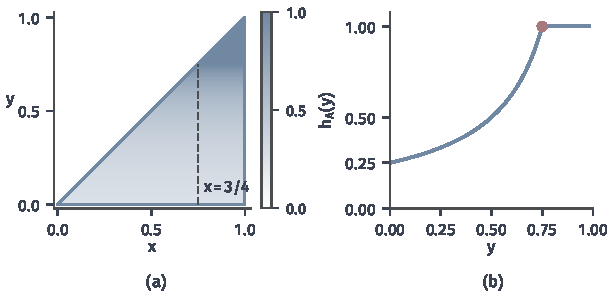
\includegraphics[width=104mm]{figures/07-probability/02-measure-theoretic-probability/matplotlib/cdis-event-function/figure.pdf}
  \caption{三角形模型中的条件概率$\mathbb{P}(X\in A\mid Y)$，$A=[\tfrac34,1]$。(a)三角形内一点$(x,y)$的颜色深浅表示$h_A(y)$，由白到蓝逐渐增大；颜色只随$y$变化，虚线$x=\tfrac34$左侧的点不在事件$\{X\in A\}$中，却与右侧同一水平线上的点取相同的值。(b)蓝线是$h_A(y)$，红点标出$y=\tfrac34$，此后$h_A=1$。}
  \label{fig:cdis-event-function}
\end{BookInlineFigure}

\paragraph{逐事件的概率规则}
条件概率是否像概率一样运算？非负、总量为一可以从条件期望的保序与线性直接得到；可数可加涉及无穷和，需要一个与积分的单调收敛定理对应的结论。

\begin{lemma}[条件单调收敛]
\label{lem:cdis-conditional-monotone}
设$0\leq Z_1\leq Z_2\leq\cdots$，$Z_n\to Z$，且$\mathbb{E}[Z]<\infty$。则$\mathbb{E}[Z_n\mid\mathcal{G}]$几乎必然递增地收敛到$\mathbb{E}[Z\mid\mathcal{G}]$。
\end{lemma}

\begin{proof}
由条件期望的保序性，对每个$n$，几乎必然有
\[
 0\leq\mathbb{E}[Z_n\mid\mathcal{G}]\leq\mathbb{E}[Z_{n+1}\mid\mathcal{G}]\leq\mathbb{E}[Z\mid\mathcal{G}].
\]
这是可数多个关系，例外集的并$N$仍是零概率集，并且$N\in\mathcal{G}$，因为它由$\mathcal{G}$可测的函数之间的比较定义。

在$N$之外令$W=\lim_n\mathbb{E}[Z_n\mid\mathcal{G}]$，在$N$上令$W=0$。$W$是$\mathcal{G}$可测函数的极限，因而$\mathcal{G}$可测，并且$0\leq W\leq\mathbb{E}[Z\mid\mathcal{G}]$几乎必然，所以可积。任取$G\in\mathcal{G}$，对递增的非负列两次使用单调收敛定理，得到
\[
 \mathbb{E}[\mathbf{1}_{G}W]=\lim_{n\to\infty}\mathbb{E}\bigl[\mathbf{1}_{G}\,\mathbb{E}[Z_n\mid\mathcal{G}]\bigr]=\lim_{n\to\infty}\mathbb{E}[\mathbf{1}_{G}Z_n]=\mathbb{E}[\mathbf{1}_{G}Z].
\]
中间的等号是条件期望在$G$上的积分恒等式。$W$满足条件期望的定义，由唯一性，$W=\mathbb{E}[Z\mid\mathcal{G}]$几乎必然。
\end{proof}

\begin{lemma}[逐事件的条件概率规则]
\label{lem:cdis-eventwise-rules}
对任意$A\in\mathcal{F}_{\mathcal{X}}$，几乎必然有$0\leq\mathbb{P}(X\in A\mid\mathcal{G})\leq1$，且$\mathbb{P}(X\in\mathcal{X}\mid\mathcal{G})=1$。对任意一列两两不交的$A_1,A_2,\ldots\in\mathcal{F}_{\mathcal{X}}$，几乎必然有
\begin{equation}
 \mathbb{P}\Bigl(X\in\bigcup_{n}A_n\Bigm|\mathcal{G}\Bigr)=\sum_{n}\mathbb{P}(X\in A_n\mid\mathcal{G}).
 \label{eq:cdis-eventwise-additivity}
\end{equation}
\end{lemma}

\begin{proof}
$0\leq\mathbf{1}_{\{X\in A\}}\leq1$，由保序性得到第一条；$\mathbf{1}_{\{X\in\mathcal{X}\}}=1$是常数，常数的条件期望是它自己。对不交的$A_n$，部分和$\sum_{k\leq n}\mathbf{1}_{\{X\in A_k\}}$递增地收敛到$\mathbf{1}_{\{X\in\cup_kA_k\}}$。由线性，部分和的条件期望是各项条件期望之和；再由引理~\ref{lem:cdis-conditional-monotone}取极限，得到式~\eqref{eq:cdis-eventwise-additivity}。
\end{proof}

引理中的“几乎必然”有一个容易忽略的限定：例外集依赖于所取的事件或事件列。对每个固定的$A$，总可以在一个零概率集之外谈论$\mathbb{P}(X\in A\mid Y=y)$；可是事件有不可数多个，不同事件的例外集合并起来可能不再是零概率集。于是出现一个问题：能否为每个$A$选定一个版本$h_A$，使对每个（或几乎每个）观测值$y$，映射$A\mapsto h_A(y)$都是$\mathcal{X}$上的一个概率分布？下面先给这样的对象一个名称。

\subsection{概率核}
\label{sec:cdis-kernel}

概率表给出了最简单的模型。传感器表按列$y$取出、除以列和，得到三个条件分布；把它们排成矩阵，每一行对应一个观测值，每行非负且和为$1$。这样的矩阵同时记录了所有目标事件的条件概率：给定$Y=y$时$X\in A$的概率，就是第$y$行在$A$中的元素之和。

\begin{BookInlineFigure}
  \centering
  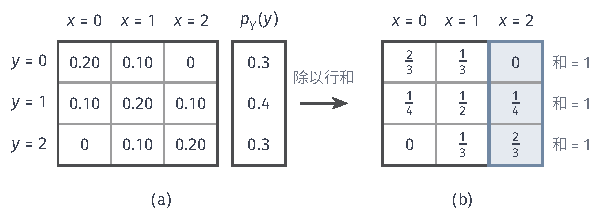
\includegraphics[width=102mm]{figures/07-probability/02-measure-theoretic-probability/tikz/cdis-table-kernel/figure.pdf}
  \caption{由传感器的联合概率表得到概率核。(a)联合概率表，行是第二台读数$y$，列是第一台读数$x$，右侧是行和$p_Y(y)$。(b)每行除以行和得到的矩阵$K(y,\{x\})$，每行是一个概率分布；浅蓝格子组成事件$\{X=2\}$所在的列，它的各行元素就是$\mathbb{P}(X=2\mid Y=y)$。}
  \label{fig:cdis-table-kernel}
\end{BookInlineFigure}

图~\ref{fig:cdis-table-kernel}画出这一步。对$A=\{2\}$，(b)中浅蓝一列给出$0,\tfrac14,\tfrac23$，正是上一小节逐个算出的条件概率；对其他事件，只要换成对应的列求和。一般情形要求的就是这样一个按观测值排列的分布族。

\begin{definition}[概率核]
\label{def:cdis-kernel}
设映射$K$对每个$y\in\mathcal{Y}$与$A\in\mathcal{F}_{\mathcal{X}}$给出一个数$K(y,A)\in[0,1]$。若
\begin{enumerate}
 \item 对每个$y\in\mathcal{Y}$，$A\mapsto K(y,A)$是$(\mathcal{X},\mathcal{F}_{\mathcal{X}})$上的概率测度；
 \item 对每个$A\in\mathcal{F}_{\mathcal{X}}$，$y\mapsto K(y,A)$是$\mathcal{F}_{\mathcal{Y}}$可测函数，
\end{enumerate}
则称$K$为从$(\mathcal{Y},\mathcal{F}_{\mathcal{Y}})$到$(\mathcal{X},\mathcal{F}_{\mathcal{X}})$的\term{概率核}（probability kernel），也称转移核。按测度的写法，$K(y,A)$也写成
\begin{equation}
 K(y,A)=\int_{A}K(y,\mathrm{d}x).
 \label{eq:cdis-kernel-notation}
\end{equation}
\end{definition}

两项要求各有用处。第一项是概率表“每行归一”的推广：固定观测值，得到一个完整的分布，事件之间的可加性对这个$y$处处成立，不再附带依赖事件的例外集。第二项保证固定事件$A$后，$K(\cdot,A)$是$\mathcal{Y}$上的可测函数，因而可以按$Y$的分布积分，例如计算$\int_{B}K(y,A)\,P_Y(\mathrm{d}y)$。$\mathcal{Y}$有限且每个子集都可测时，第二项自动成立，所以在概率表中只看得到第一项。

第二项并非多余。设$S\subseteq[0,1]$不是Borel集，令$y\in S$时$K(y,\cdot)$是$\{1\}$上的单点分布，其余$y$时是$\{0\}$上的单点分布。每个$K(y,\cdot)$都是概率测度，但$y\mapsto K(y,\{1\})=\mathbf{1}_{S}(y)$不可测，积分$\int K(y,\{1\})\,P_Y(\mathrm{d}y)$没有意义。这样的$K$无法用来“按观测加权”，也就谈不上与联合规律相容。

\paragraph{三角形模型的核}
三角形模型中，对$0\leq y<1$令$K(y,\cdot)$为$[y,1]$上的均匀分布，记$\lambda$为长度，则
\[
 K(y,A)=\frac{\lambda(A\cap[y,1])}{1-y},\qquad 0\leq y<1,
\]
在$y=1$等其余点令$K(y,\cdot)$为$\{1\}$上的单点分布。固定$y$，这是一个概率测度。固定$A$，函数$y\mapsto\lambda(A\cap[y,1])$连续，因而$K(\cdot,A)$在$[0,1)$上可测，补上可测的余下部分后整体可测。

图~\ref{fig:cdis-kernel-views}从两个方向看同一个核。(a)固定观测值，曲线是分布函数$t\mapsto K(y,[0,t])$：每个$y$对应一个完整的分布。(b)固定事件，曲线是观测值的函数$y\mapsto K(y,A)$：每个事件对应一个可测函数。概率核的定义就是要求这两个方向同时成立。

\begin{BookInlineFigure}
  \centering
  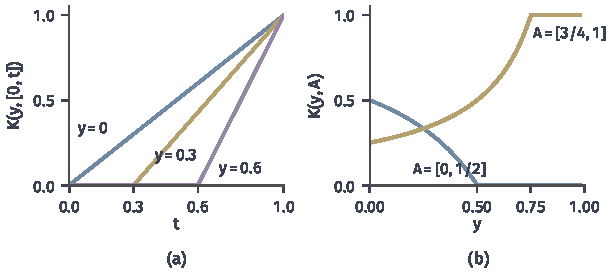
\includegraphics[width=104mm]{figures/07-probability/02-measure-theoretic-probability/matplotlib/cdis-kernel-views/figure.pdf}
  \caption{三角形模型的概率核$K(y,\cdot)=\operatorname{Unif}(y,1)$的两种读法。(a)固定$y=0,0.3,0.6$（蓝、黄、紫），横轴为$t$，曲线为$K(y,[0,t])$，每条都是一个分布函数。(b)固定事件$A=[0,\tfrac12]$（蓝）与$A=[\tfrac34,1]$（黄），曲线为$y\mapsto K(y,A)$。}
  \label{fig:cdis-kernel-views}
\end{BookInlineFigure}

\paragraph{核对函数与对测度的作用}
概率表的核是行和为一的非负矩阵，它可以从右边乘列向量，也可以从左边乘行向量。一般的核同样有这两种作用。对有界可测函数$g$，令$(Kg)(y)=\int g(x)\,K(y,\mathrm{d}x)$，这是“观测为$y$时$g$的平均”；对$\mathcal{Y}$上的概率测度$\mu$，令$(\mu K)(A)=\int K(y,A)\,\mu(\mathrm{d}y)$，这是“先按$\mu$抽观测值、再按核抽目标”时目标的分布。第~\ref{sec:cdis-integration}节与第~\ref{sec:cdis-joint}节分别研究这两种作用；概率表中它们就是矩阵乘列向量与行向量乘矩阵。

\subsection{正则条件分布}
\label{sec:cdis-regular}

概率核本身只是一族按观测值排列的分布，与$X$、$Y$的联合规律还没有关系。任意一个核都满足定义~\ref{def:cdis-kernel}，例如对所有$y$都取同一个分布。要让它成为“给定$Y$时$X$的分布”，必须要求它在每个事件上给出的值就是条件概率。

\begin{definition}[正则条件分布]
\label{def:cdis-regular}
从$\mathcal{Y}$到$\mathcal{X}$的概率核$K$若对每个$A\in\mathcal{F}_{\mathcal{X}}$满足
\begin{equation}
 K(Y,A)=\mathbb{P}(X\in A\mid Y)\quad\text{几乎必然},
 \label{eq:cdis-regular}
\end{equation}
则称$K$为给定$Y$时$X$的\term{正则条件分布}（regular conditional distribution），也记作$P_{X\mid Y}(A\mid y)=K(y,A)$。
\end{definition}

式~\eqref{eq:cdis-regular}中的例外集仍然可以随$A$改变，这一点与逐事件的条件概率相同。差别在于，核对每个$y$都是概率测度：正则条件分布是从条件概率的众多版本中挑出的一组，使得在每个观测值处都拼成一个分布。“正则”指的就是这种可以拼合的性质。给定一般的信息$\mathcal{G}$时，把$\mathcal{Y}$换成$(\Omega,\mathcal{G})$、$Y$换成恒等映射，同样可以定义给定$\mathcal{G}$的正则条件分布，本章主要讨论给定随机对象$Y$的情形。

验证一个核是否满足式~\eqref{eq:cdis-regular}，按条件期望的定义需要检查$\sigma(Y)$中的每个事件。$\sigma(Y)$的事件都形如$\{Y\in B\}$，把这一检查写成$\mathcal{Y}$上的积分，得到一个便于计算的判别。

\begin{lemma}[正则条件分布的积分判别]
\label{lem:cdis-regular-criterion}
概率核$K$是给定$Y$时$X$的正则条件分布，当且仅当对一切$A\in\mathcal{F}_{\mathcal{X}}$、$B\in\mathcal{F}_{\mathcal{Y}}$，
\begin{equation}
 \mathbb{P}(X\in A,\ Y\in B)=\int_{B}K(y,A)\,P_Y(\mathrm{d}y).
 \label{eq:cdis-regular-criterion}
\end{equation}
\end{lemma}

\begin{proof}
固定$A$。$K(\cdot,A)$可测且取值于$[0,1]$，所以$K(Y,A)$是$\sigma(Y)$可测的有界随机变量。按条件期望的定义，式~\eqref{eq:cdis-regular}成立当且仅当对每个$\{Y\in B\}\in\sigma(Y)$，
\[
 \mathbb{E}\bigl[\mathbf{1}_{\{Y\in B\}}K(Y,A)\bigr]=\mathbb{E}\bigl[\mathbf{1}_{\{Y\in B\}}\mathbf{1}_{\{X\in A\}}\bigr].
\]
右边是$\mathbb{P}(X\in A,\ Y\in B)$。左边的被积函数是$Y$的函数$\mathbf{1}_{B}(y)K(y,A)$，由分布的积分公式（第~\ref{chap:probability-spaces}章），它等于$\int_{B}K(y,A)\,P_Y(\mathrm{d}y)$。两边相等就是式~\eqref{eq:cdis-regular-criterion}。
\end{proof}

式~\eqref{eq:cdis-regular-criterion}说的是：按观测的分布把各个$y$处的条件概率加权累计，必须回到联合概率。这正是“条件化是缩小样本范围再重新归一”的反向检验：把各组重新归一的结果乘回组的质量，应当恢复原来的质量分配。

\paragraph{与概率表和条件密度相容}
有概率表时，取$K(y,\{x\})=p_{X,Y}(x,y)/p_Y(y)$（$p_Y(y)>0$），$p_Y(y)=0$的$y$上任取一个分布。代入式~\eqref{eq:cdis-regular-criterion}的右边，零概率的$y$不贡献，于是
\[
 \sum_{y\in B}p_Y(y)\sum_{x\in A}\frac{p_{X,Y}(x,y)}{p_Y(y)}=\sum_{y\in B}\sum_{x\in A}p_{X,Y}(x,y)=\mathbb{P}(X\in A,\ Y\in B).
\]
第~\ref{chap:random-vectors}章的条件质量函数确实给出正则条件分布。

三角形模型中，$P_Y$有密度$f_Y(y)=2(1-y)$。代入上一小节的核，对$y<1$，$K(y,A)f_Y(y)=2\lambda(A\cap[y,1])$，所以
\[
 \int_{B}K(y,A)\,f_Y(y)\,\mathrm{d}y=\int_{B}\int_{A}2\cdot\mathbf{1}_{\{x\geq y\}}\,\mathrm{d}x\,\mathrm{d}y=\mathbb{P}(X\in A,\ Y\in B).
\]
最后一步是联合密度在$A\times B$上的积分，交换次序的依据是Tonelli定理。一般的条件密度公式在第~\ref{sec:cdis-zero-probability}小节用同样的方法验证。

\paragraph{没有联合密度的情形}
密度比并不是正则条件分布的必要形式。设$Y\sim\operatorname{Unif}(0,1)$，$X=Y$。$(X,Y)$的全部质量落在对角线上，对角线的面积为零，联合密度不存在。直觉上，知道$Y=y$就知道$X=y$，所以应取$K(y,\cdot)=\delta_y$，即$\{y\}$上的单点分布。核对式~\eqref{eq:cdis-regular-criterion}：
\[
 \int_{B}\delta_y(A)\,P_Y(\mathrm{d}y)=P_Y(A\cap B)=\mathbb{P}(Y\in A,\ Y\in B)=\mathbb{P}(X\in A,\ Y\in B).
\]
式~\eqref{eq:cdis-regular-criterion}成立。核$\delta_y$可测：$y\mapsto\delta_y(A)=\mathbf{1}_{A}(y)$对Borel集$A$是可测函数。这个例子说明，正则条件分布的定义不依赖密度，只依赖联合规律本身。


\section{存在性与版本}
\label{sec:cdis-existence}

正则条件分布要求一个概率核同时给出所有事件的条件概率。逐事件的条件概率总是存在，但每个都只在各自的零概率集之外唯一，拼合时可能出问题。这一节先用一个例子说明随意挑选版本会怎样失败，再给出正则条件分布存在的条件，然后说明它在什么意义下唯一，最后讨论单个零概率观测值上的取值。

\subsection{存在条件}
\label{sec:cdis-existence-conditions}

\paragraph{随意挑选版本的失败}
仍取$Y\sim\operatorname{Unif}(0,1)$、$X=Y$。对每个单点$a\in[0,1]$，事件$\{X=a\}$的概率为零，指示函数几乎必然为零，所以常数$0$是$\mathbb{P}(X=a\mid Y)$的一个合法版本，即可以取$h_{\{a\}}\equiv0$。对每个区间$I$，取$h_{I}(y)=\mathbf{1}_{I}(y)$，这也是合法版本。

现在固定任意一个观测值$y$，看这些版本能否在$y$处拼成一个分布。若概率测度$\mu$在所有区间上满足$\mu(I)=\mathbf{1}_{I}(y)$，则$\mu$与$\delta_y$在区间上相同；区间对有限交封闭并生成Borel集，由测度在生成$\pi$系统上的唯一性，$\mu=\delta_y$，于是$\mu(\{y\})=1$。可是挑出的版本给单点$\{y\}$的值是$0$。这组版本在\emph{每一个}$y$处都拼不成分布，见图~\ref{fig:cdis-version-collapse}。

\begin{BookInlineFigure}
  \centering
  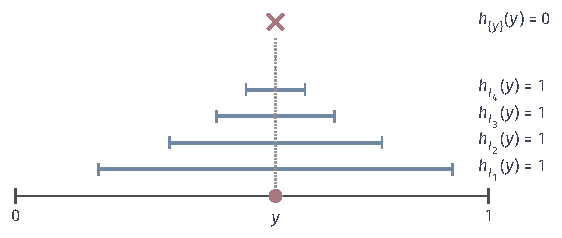
\includegraphics[width=95mm]{figures/07-probability/02-measure-theoretic-probability/tikz/cdis-version-collapse/figure.pdf}
  \caption{随意挑选版本的失败，$X=Y\sim\operatorname{Unif}(0,1)$。固定观测值$y$（红点），包含$y$的区间（蓝线）逐个缩小，所选版本都给出$1$；单点$\{y\}$所选的版本是$0$（红叉）。可数可加性要求区间上的值递减到单点上的值，二者矛盾。}
  \label{fig:cdis-version-collapse}
\end{BookInlineFigure}

每个单点事件的版本只在零概率集$\{Y=a\}$上“出错”，单独看都没有问题；不可数多个这样的零概率集合并起来却覆盖了整个$[0,1]$。补救的思路是：只对可数个事件选版本，可数个零概率集的并仍是零概率集；再用这可数个事件把整个分布确定下来。在实轴上，有理数处的分布函数值就足够确定一个分布。

\paragraph{实值目标}
先处理$X$取实数值的情形。观测$Y$的取值空间不需要任何结构。

\begin{theorem}[实值随机变量的正则条件分布]
\label{thm:cdis-existence-real}
设$X$是实随机变量，$Y$取值于任意可测空间$(\mathcal{Y},\mathcal{F}_{\mathcal{Y}})$。则存在给定$Y$时$X$的正则条件分布，即存在从$\mathcal{Y}$到$(\mathbb{R},\mathcal{B}(\mathbb{R}))$的概率核$K$，使对每个Borel集$A$，$K(Y,A)=\mathbb{P}(X\in A\mid Y)$几乎必然成立。
\end{theorem}

\begin{proof}
证明分四步：在有理数上选版本，收集可数个关系，修正成分布函数，最后核对可测性与版本性质。

第一步，选版本。对每个有理数$q$，由式~\eqref{eq:cdis-function-representation}取可测函数$G_q:\mathcal{Y}\to[0,1]$，使$G_q(Y)=\mathbb{P}(X\leq q\mid Y)$几乎必然。

第二步，收集关系。下面每条都由一个已知结论保证几乎必然成立：
\begin{enumerate}
 \item 对有理数$q<r$，$G_q(Y)\leq G_r(Y)$，由条件期望的保序性；
 \item 对每个有理数$q$，$G_{q+1/n}(Y)\to G_q(Y)$（$n\to\infty$），对递增到$\mathbf{1}_{\{X>q\}}$的$\mathbf{1}_{\{X>q+1/n\}}$用引理~\ref{lem:cdis-conditional-monotone}，再用线性；
 \item $G_{-n}(Y)\to0$，$G_{n}(Y)\to1$（$n\to\infty$），理由同上。
\end{enumerate}
令$N$为使上述某条关系不成立的$y$的全体。每条关系不成立的$y$构成$\mathcal{F}_{\mathcal{Y}}$中的可测集，因为它们由可数个可测函数$G_q$定义；关系几乎必然成立，说明这个集合的$P_Y$测度为零。关系一共可数条，所以$N$可测，并且$P_Y(N)=0$。

第三步，修正。对$y\notin N$，令
\[
 F(t\mid y)=\inf\{G_q(y):q\in\mathbb{Q},\ q>t\},\qquad t\in\mathbb{R}.
\]
由第1条，$F(\cdot\mid y)$不减；作为$q>t$上的下确界，它右连续。由第1、2条，在有理数$q$处$F(q\mid y)=\lim_nG_{q+1/n}(y)=G_q(y)$。由第3条，$t\to-\infty$时$F\to0$，$t\to+\infty$时$F\to1$。所以$F(\cdot\mid y)$是一个分布函数，对应$\mathbb{R}$上唯一的概率测度，记为$K(y,\cdot)$。对$y\in N$，令$K(y,\cdot)=\delta_0$。

第四步，核对。先看可测性。对实数$t$，取有理数$q_n\downarrow t$，则
\[
 K(y,(-\infty,t])=\mathbf{1}_{N^{\mathrm{c}}}(y)\lim_{n\to\infty}G_{q_n}(y)+\mathbf{1}_{N}(y)\,\mathbf{1}_{\{t\geq0\}},
\]
是可测函数的极限与组合，所以可测。使$y\mapsto K(y,A)$可测的Borel集$A$的全体对补集（$K(y,A^{\mathrm{c}})=1-K(y,A)$）和不交可数并（可测函数之和）封闭，含$\mathbb{R}$，是$\lambda$系统；它包含对有限交封闭的半直线族，由$\pi$--$\lambda$定理包含全部Borel集。

再看版本性质。对有理数$q$，在$\{Y\notin N\}$上$K(Y,(-\infty,q])=G_q(Y)$，所以$K(Y,(-\infty,q])=\mathbb{P}(X\leq q\mid Y)$几乎必然。对实数$t$与$q_n\downarrow t$，左边由测度的连续性收敛到$K(Y,(-\infty,t])$，右边由第二步的同一论证几乎必然收敛到$\mathbb{P}(X\leq t\mid Y)$，两者几乎必然相等。使$K(Y,A)=\mathbb{P}(X\in A\mid Y)$几乎必然成立的$A$的全体，由线性与引理~\ref{lem:cdis-eventwise-rules}对补集和不交可数并封闭，同样是含半直线族的$\lambda$系统，于是包含全部Borel集。
\end{proof}

证明的关键在第二步：所有要求都写成可数条，例外集只并了可数次。第三步的下确界把“只在有理数上知道的值”补成右连续的分布函数，在例外集$N$上则直接换成一个固定的分布。图~\ref{fig:cdis-rational-thresholds}用三角形模型画出这两种情形。

\begin{BookInlineFigure}
  \centering
  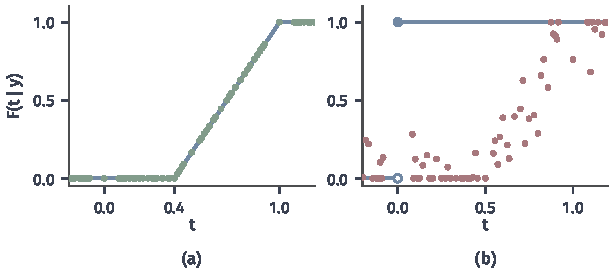
\includegraphics[width=104mm]{figures/07-probability/02-measure-theoretic-probability/matplotlib/cdis-rational-thresholds/figure.pdf}
  \caption{由有理阈值构造条件分布函数（三角形模型）。(a)$y=0.4$不在例外集中：绿点是分母不超过$12$的有理数$q$处的值$G_q(y)$，蓝线是由下确界得到的$F(t\mid y)$，即$[0.4,1]$上均匀分布的分布函数。(b)在一个零概率的观测值上，若所选版本的值（红点）不单调，该点划入例外集，改用固定的分布$\delta_0$（蓝线）。}
  \label{fig:cdis-rational-thresholds}
\end{BookInlineFigure}

\paragraph{标准Borel空间}
证明只用到实轴的两个性质：有一列可数的事件生成全部Borel集，并且在这列事件上相容的值能补成一个测度。许多取值空间可以搬到实轴上而保留这些性质。

\begin{definition}[标准Borel空间]
\label{def:cdis-standard-borel}
可测空间$(\mathcal{X},\mathcal{F}_{\mathcal{X}})$若存在Borel集$S\subseteq\mathbb{R}$与双射$\varphi:\mathcal{X}\to S$，使$\varphi$与$\varphi^{-1}$都可测（$S$取相对Borel $\sigma$代数），则称它为\term{标准Borel空间}（standard Borel space），$\varphi$称为\term{Borel同构}（Borel isomorphism）。
\end{definition}

有限集与可数集（每个子集都可测）满足定义：把元素依次编号为$1,2,\dots$，编号映射与它的逆都可测。更一般地，带Borel $\sigma$代数的完备可分度量空间都是标准Borel空间，其中包括$\mathbb{R}^{d}$、矩阵空间、它们的Borel子集，以及标准Borel空间的可数乘积。这一结论的证明需要用到描述集合论中关于Borel集像的定理，篇幅较长，读者可查阅~\scite{math-kallenberg2021probability}。

它的含义可以从$[0,1)^{2}$看出。把两个坐标写成二进制小数，再把两串数字交替排成一串，就得到$[0,1)$中的一个数，见图~\ref{fig:cdis-digit-interleave}。这个映射把平面上的点一对一地编成一个实数，前$2k$位数字只依赖两个坐标的前$k$位，所以它和它的逆都可测。证明中需要额外处理的只是二进制展开不唯一的那些点，它们构成一个可数集。

\begin{BookInlineFigure}
  \centering
  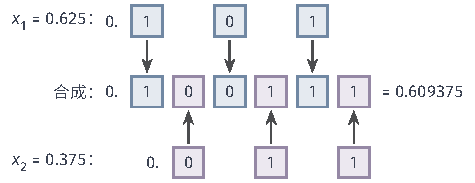
\includegraphics[width=80mm]{figures/07-probability/02-measure-theoretic-probability/tikz/cdis-digit-interleave/figure.pdf}
  \caption{交替排列二进制数字，把$[0,1)^{2}$中的点$(x_1,x_2)$编成$[0,1)$中的一个数。蓝色数字是$x_1=0.625$的二进制位，紫色数字是$x_2=0.375$的二进制位，两串数字$101$与$011$交替排成$100111$，合成的二进制小数$0.100111$等于$0.609375$。}
  \label{fig:cdis-digit-interleave}
\end{BookInlineFigure}

\begin{theorem}[正则条件分布的存在性]
\label{thm:cdis-existence}
设$X$取值于标准Borel空间$(\mathcal{X},\mathcal{F}_{\mathcal{X}})$，$Y$取值于任意可测空间$(\mathcal{Y},\mathcal{F}_{\mathcal{Y}})$，特别地，$\mathcal{Y}$可以是标准Borel空间。则给定$Y$时$X$的正则条件分布存在。
\end{theorem}

\begin{proof}
取Borel同构$\varphi:\mathcal{X}\to S$，令$X'=\varphi(X)$，它是实随机变量。由定理~\ref{thm:cdis-existence-real}，存在给定$Y$时$X'$的正则条件分布$K'$。因为$X'\in S$必然成立，$K'(Y,S)=\mathbb{P}(X'\in S\mid Y)=1$几乎必然，于是集合$N=\{y:K'(y,S)<1\}$可测且$P_Y(N)=0$。

固定一点$x_0\in\mathcal{X}$，令
\[
 K(y,A)=\begin{cases}K'\bigl(y,\varphi(A)\bigr), & y\notin N,\\ \delta_{x_0}(A), & y\in N.\end{cases}
\]
$\varphi(A)=(\varphi^{-1})^{-1}(A)$是$S$的Borel子集，所以右边有意义。$y\notin N$时，$K'(y,\cdot)$的质量全在$S$上，$\varphi$又是双射，$A\mapsto K'(y,\varphi(A))$就是$K'(y,\cdot)$在$S$上的部分经$\varphi^{-1}$推前得到的概率测度。可测性由$K'$继承。最后，$\{X\in A\}=\{X'\in\varphi(A)\}$，所以
\[
 \begin{aligned}
 K(Y,A)&=K'\bigl(Y,\varphi(A)\bigr)=\mathbb{P}\bigl(X'\in\varphi(A)\bigm|Y\bigr)\\
 &=\mathbb{P}(X\in A\mid Y)\quad\text{几乎必然}.
 \end{aligned}\qedhere
\]
\end{proof}

比较一下两种存在性。对单个可积随机变量，条件期望总是存在，第~\ref{chap:conditional-expectation}章用Radon--Nikodym定理构造它，不要求取值空间有任何结构。正则条件分布要把不可数多个条件概率拼在一起，需要目标空间提供一列可数的生成事件以及从这些事件上的值恢复测度的能力；标准Borel条件同时提供了这两点。在没有这类结构的一般可测空间上，可以构造出正则条件分布不存在的例子，构造要用到不可测集，篇幅较长。本卷遇到的取值空间（实数、向量、矩阵、有限或可数的符号集，以及它们的有限或可数乘积）都是标准Borel空间，以后把这一条件作为默认设定，在需要时说明。

\subsection{几乎处处唯一性}
\label{sec:cdis-uniqueness}

正则条件分布找到了一个，是否还有别的？在一个$P_Y$零测集上改动核，积分判别~\eqref{eq:cdis-regular-criterion}察觉不到，问题是除此之外还有没有更大的自由。

\begin{theorem}[正则条件分布的几乎处处唯一性]
\label{thm:cdis-uniqueness}
设$X$取值于标准Borel空间，$K$与$K'$都是给定$Y$时$X$的正则条件分布。则存在$N\in\mathcal{F}_{\mathcal{Y}}$，$P_Y(N)=0$，使对一切$y\notin N$，$K(y,\cdot)=K'(y,\cdot)$。
\end{theorem}

\begin{proof}
先取一个可数且对有限交封闭的事件族$\mathcal{P}$，它生成$\mathcal{F}_{\mathcal{X}}$。$\mathcal{X}=\mathbb{R}$时取$\{(-\infty,q]:q\in\mathbb{Q}\}$；一般情形取Borel同构$\varphi$，令$\mathcal{P}$为这些半直线的原像$\varphi^{-1}((-\infty,q])$的全体，$q\in\mathbb{Q}$。

对每个$P\in\mathcal{P}$，两个核都是$\mathbb{P}(X\in P\mid Y)$的版本，所以$K(Y,P)=K'(Y,P)$几乎必然，即集合$N_P=\{y:K(y,P)\neq K'(y,P)\}$满足$P_Y(N_P)=0$。令$N=\bigcup_{P\in\mathcal{P}}N_P$，它是可数个零测集的并，$P_Y(N)=0$。对$y\notin N$，两个概率测度$K(y,\cdot)$与$K'(y,\cdot)$在生成$\pi$系统$\mathcal{P}$上取值相同，由测度在生成$\pi$系统上的唯一性（可参考\BookChapterRef{chap:measure}{卷四第5章“测度”}），它们在$\mathcal{F}_{\mathcal{X}}$上相同。
\end{proof}

与存在性的证明一样，关键是把比较压缩到可数个事件上，使例外集只并可数次。结论中的例外集用观测的分布$P_Y$来衡量，而不是用$\mathcal{Y}$上的某种“体积”。

\paragraph{单个观测值上的取值}
定理~\ref{thm:cdis-uniqueness}的反面同样重要：联合规律只决定核的$P_Y$等价类，不决定它在某个特定零测点上的值。三角形模型中，把$y=\tfrac12$处的分布换成$\delta_0$，得到核$K'$。$P_Y(\{\tfrac12\})=0$，式~\eqref{eq:cdis-regular-criterion}中积分不受影响，$K'$仍是正则条件分布；可是$K'(\tfrac12,\cdot)$说“给定$Y=\tfrac12$时$X=0$”，而$X\geq Y$本应必然成立。同样可以在所有有理数$y$上改动，甚至在零测的Cantor集上改动。

改动不能扩大到正测度的观测集上。若在$y\in[\tfrac14,\tfrac12]$上把核换成$\operatorname{Unif}(0,1)$，取$A=[0,\tfrac18]$、$B=[\tfrac14,\tfrac12]$。三角形中$X\geq Y\geq\tfrac14$，所以$\mathbb{P}(X\in A,\ Y\in B)=0$，而改动后的核给出
\[
 \int_{1/4}^{1/2}\frac18\cdot2(1-y)\,\mathrm{d}y=\frac14\int_{1/4}^{1/2}(1-y)\,\mathrm{d}y=\frac14\cdot\frac{5}{32}=\frac{5}{128}>0 ,
\]
式~\eqref{eq:cdis-regular-criterion}不成立。图~\ref{fig:cdis-two-versions}对照了两种改动。

\begin{BookInlineFigure}
  \centering
  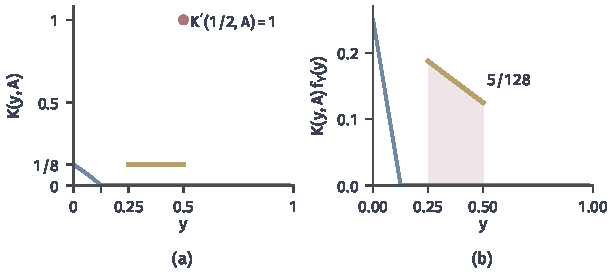
\includegraphics[width=104mm]{figures/07-probability/02-measure-theoretic-probability/matplotlib/cdis-two-versions/figure.pdf}
  \caption{三角形模型中$A=[0,\tfrac18]$时核的几种取法。(a)蓝线是由密度比得到的$y\mapsto K(y,A)$，在$y\geq\tfrac18$时为零；红点是只在$y=\tfrac12$一个点上的改动，它仍给出正则条件分布；黄线把$[\tfrac14,\tfrac12]$整段改成$\tfrac18$。(b)式~\eqref{eq:cdis-regular-criterion}中的被积函数$K(y,A)f_Y(y)$：单点改动不影响积分，黄线的改动多出浅红区域的质量$\tfrac{5}{128}$，不再是正则条件分布。}
  \label{fig:cdis-two-versions}
\end{BookInlineFigure}

若某个观测值本身有正概率，$P_Y(\{y_0\})>0$，它不可能落在零测例外集中，$K(y_0,\cdot)$就被唯一确定，并且由式~\eqref{eq:cdis-regular-criterion}取$B=\{y_0\}$，
\[
 K(y_0,A)=\frac{\mathbb{P}(X\in A,\ Y=y_0)}{\mathbb{P}(Y=y_0)},
\]
这正是第~\ref{chap:classical-probability}章的条件概率。正则条件分布在有正概率的观测值上与初等条件概率一致，额外的自由只出现在零概率的观测值上。

\subsection{零概率条件}
\label{sec:cdis-zero-probability}

$Y$连续时，每个单点的概率都是零，$\mathbb{P}(X\in A\mid Y=y)$不能写成两个事件概率之比。正则条件分布给这个记号一个意义：它就是$K(y,A)$，作为$y$的函数在$P_Y$几乎处处的意义下由联合规律确定。下面先说明密度公式给出一个版本，再讨论单个零概率观测值上附加的选择。

\paragraph{密度公式给出的版本}
设$\alpha,\beta$分别是$\mathcal{X},\mathcal{Y}$上的$\sigma$有限测度，例如Lebesgue测度或计数测度，$(X,Y)$关于乘积测度$\alpha\otimes\beta$有联合密度$f$。记$f_Y(y)=\int f(x,y)\,\alpha(\mathrm{d}x)$为$Y$关于$\beta$的密度。

\begin{theorem}[条件密度给出的正则条件分布]
\label{thm:cdis-density-version}
在上述设定下，任取$\mathcal{X}$上的概率测度$\nu_0$，令
\begin{equation}
 K(y,A)=\begin{cases}
 \dfrac{1}{f_Y(y)}\displaystyle\int_{A}f(x,y)\,\alpha(\mathrm{d}x), & 0<f_Y(y)<\infty,\\
 \nu_0(A), & \text{其他}.
 \end{cases}
 \label{eq:cdis-density-version}
\end{equation}
则$K$是给定$Y$时$X$的正则条件分布。
\end{theorem}

\begin{proof}
对$0<f_Y(y)<\infty$的$y$，$K(y,\cdot)$是非负函数$f(\cdot,y)/f_Y(y)$关于$\alpha$的不定积分，总量为$1$，是概率测度；其余$y$处是$\nu_0$。由Tonelli定理，$y\mapsto\int_{A}f(x,y)\,\alpha(\mathrm{d}x)$与$f_Y$都可测，集合$\{0<f_Y<\infty\}$可测，所以$K(\cdot,A)$可测，$K$是概率核。

再核对式~\eqref{eq:cdis-regular-criterion}。$\int f_Y\,\mathrm{d}\beta=1$，所以$\{f_Y=\infty\}$是$\beta$零测集；$\{f_Y=0\}$上被积函数含因子$f_Y=0$。于是这两部分都不贡献，
\[
 \begin{aligned}
 \int_{B}K(y,A)\,f_Y(y)\,\beta(\mathrm{d}y)&=\int_{B}\int_{A}f(x,y)\,\alpha(\mathrm{d}x)\,\beta(\mathrm{d}y)\\
 &=\mathbb{P}(X\in A,\ Y\in B).
 \end{aligned}
\]
由引理~\ref{lem:cdis-regular-criterion}，$K$是正则条件分布。
\end{proof}

定理同时涵盖了概率表（$\alpha,\beta$都取计数测度）、条件密度（都取Lebesgue测度），以及离散状态与连续读数的混合模型（一个取计数测度，一个取Lebesgue测度）。证明没有用到标准Borel条件：有了联合密度，核可以直接写出来。

公式~\eqref{eq:cdis-density-version}在每个$y$处都给出一个值，但这个值依赖所选的密度$f$。联合密度只在$\alpha\otimes\beta$零测集之外确定；在直线$\{y=y_0\}$上任意改动$f$，联合规律不变，$K(y_0,\cdot)$却变了。单个零概率观测值上的条件分布需要额外的要求来选定。

\paragraph{连续性的要求}
常用的要求是连续性。第~\ref{chap:random-vectors}章证明：若联合密度在$y_0$附近连续且$f_Y(y_0)>0$，窄带$\{y_0\leq Y\leq y_0+h\}$上的条件概率在$h\to0$时趋于密度比。这个极限选出了一个特定的值。设$\mathcal{Y}=\mathbb{R}$。若两个版本对定理~\ref{thm:cdis-uniqueness}证明中可数生成族的每个事件$P$，$y\mapsto K(y,P)$都在$y_0$处连续，并且$y_0$的每个邻域都有正的$P_Y$质量，那么两个版本在$y_0$处相同：它们在一个$P_Y$零测集之外相等，每个邻域里都有这样的点，取极限即得两者在每个$P$上的值相同，再由生成$\pi$系统上的唯一性得到$K(y_0,\cdot)$相同。

这种选择有两个限度。其一，满足要求的版本未必存在。设$Y\sim\operatorname{Unif}(-1,1)$，$X=\mathbf{1}_{\{Y>0\}}$。正则条件分布在$y<0$时是$\delta_0$，在$y>0$时是$\delta_1$（几乎处处唯一），$y=0$处无论取什么，$y\mapsto K(y,\{1\})$都不连续，见图~\ref{fig:cdis-no-continuous}。连续性在这里无法选出$K(0,\cdot)$，这一点的值只能另作约定。

\begin{BookInlineFigure}
  \centering
  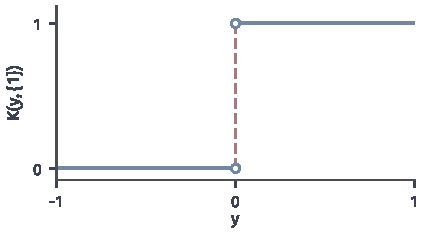
\includegraphics[width=72mm]{figures/07-probability/02-measure-theoretic-probability/matplotlib/cdis-no-continuous/figure.pdf}
  \caption{$Y\sim\operatorname{Unif}(-1,1)$、$X=\mathbf{1}_{\{Y>0\}}$时的$y\mapsto K(y,\{1\})$。蓝线在$y<0$时为$0$，在$y>0$时为$1$；$y=0$处（红色虚线上的任何值）怎样取都不能使它连续。}
  \label{fig:cdis-no-continuous}
\end{BookInlineFigure}

其二，选出的值依赖用哪个观测量逼近同一个零概率事件。设$(X,Y)$在单位正方形上均匀分布，问“给定$X=Y$时$X$的分布”。事件$\{X=Y\}$可以写成$\{D=0\}$，其中$D=Y-X$；也可以写成$\{R=1\}$，其中$R=Y/X$。两种写法描述同一条对角线，给出的条件分布却不同。

\paragraph{两种逼近的计算}
先用$D$。由换元$(x,y)\mapsto(x,d)=(x,y-x)$，Jacobian行列式为$1$，$(X,D)$的联合密度是
\[
 f_{X,D}(x,d)=1,\qquad 0<x<1,\ 0<x+d<1 .
\]
在$d=0$处它对$x\in(0,1)$恒为$1$，边缘$f_D(0)=1$，由式~\eqref{eq:cdis-density-version}，给定$D=0$时$X$的条件密度是$1$，即$X\sim\operatorname{Unif}(0,1)$。

再用$R$。由换元$(x,y)\mapsto(x,r)=(x,y/x)$，逆变换$y=rx$的Jacobian行列式为$x$，$(X,R)$的联合密度是
\[
 f_{X,R}(x,r)=x,\qquad 0<x<1,\ 0<rx<1 .
\]
在$r=1$处它是$x$，边缘$f_R(1)=\int_0^1x\,\mathrm{d}x=\tfrac12$，所以给定$R=1$时$X$的条件密度是$2x$。两个结果都由连续的联合密度得到，都是各自观测量下“连续性选出的”版本，却互不相同。

图~\ref{fig:cdis-borel-kolmogorov}说明差别从哪里来。$\{\lvert D\rvert\leq h\}$是沿对角线等宽的带子，各处收进同样多的质量；$\{\lvert R-1\rvert\leq h\}$是从原点张开的楔形，离原点越远越宽，收进的质量与$x$成正比。两种窄化在极限下落在同一条线上，但沿线分配质量的权重不同。这一现象称为\term{Borel--Kolmogorov悖论}（Borel--Kolmogorov paradox）。

\begin{BookInlineFigure}
  \centering
  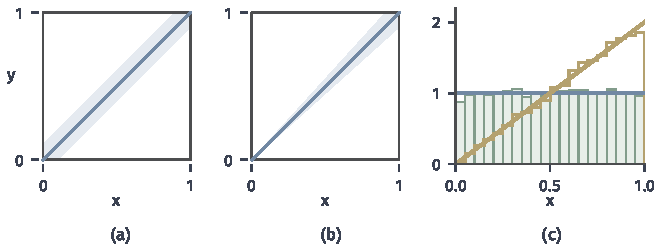
\includegraphics[width=112mm]{figures/07-probability/02-measure-theoretic-probability/matplotlib/cdis-borel-kolmogorov/figure.pdf}
  \caption{同一条对角线的两种逼近，$(X,Y)$在单位正方形上均匀分布。(a)浅蓝带子$\{\lvert Y-X\rvert\leq h\}$，$h=0.1$。(b)浅蓝楔形$\{\lvert Y/X-1\rvert\leq h\}$，$h=0.1$。(c)固定种子$7$模拟$4\times10^{5}$个点，取$h=0.02$：落在带子中的点的$X$坐标直方图为浅绿柱，落在楔形中的为黄色阶梯线；蓝线与黄线是极限密度$1$与$2x$。}
  \label{fig:cdis-borel-kolmogorov}
\end{BookInlineFigure}

悖论并不说明理论有矛盾。条件分布总是“给定某个观测量$Y$”的分布，它是$\mathcal{Y}$上的一个核，只在$P_Y$几乎处处的意义下确定。$D$与$R$是两个不同的观测量，生成不同的信息，给定$D$与给定$R$的条件分布是两个不同的核；它们在各自零概率点$d=0$、$r=1$上的值，分别依赖各自的选择方式。脱离观测量单独说“给定零概率事件$\{X=Y\}$”，没有确定的意义。在零概率观测值上用连续性等要求选值时，必须指明观测量，核对满足要求的版本存在，并清楚所得的值是一种约定，而不是由联合规律推出的结论。


\section{条件分布的积分}
\label{sec:cdis-integration}

固定观测值$y$，$K(y,\cdot)$是一个普通的概率测度，可以对它积分。这样得到的$\int g(x)\,K(y,\mathrm{d}x)$是“观测为$y$时$g(X)$的平均”。它与第~\ref{chap:conditional-expectation}章的条件期望$\mathbb{E}[g(X)\mid Y]$是什么关系？这一节证明，在可积条件下两者几乎必然相等，再用这个表示计算条件矩。

条件期望仍以第~\ref{chap:conditional-expectation}章的积分刻画为定义，它对任何可积随机变量都存在；下面的表示只在正则条件分布存在时才可用，它提供的是一个计算方法和一个对每个$y$都有定义的版本。

\subsection{条件期望的积分表示}
\label{sec:cdis-integral-representation}

\begin{theorem}[条件期望的积分表示]
\label{thm:cdis-integral-representation}
设$K$是给定$Y$时$X$的正则条件分布，$g:\mathcal{X}\to\mathbb{R}$可测，$\mathbb{E}\lvert g(X)\rvert<\infty$。则对$P_Y$几乎每个$y$，$\int\lvert g(x)\rvert\,K(y,\mathrm{d}x)<\infty$，并且
\begin{equation}
 \mathbb{E}[g(X)\mid Y]=\int g(x)\,K(Y,\mathrm{d}x)\quad\text{几乎必然}.
 \label{eq:cdis-integral-representation}
\end{equation}
在使积分不收敛的$P_Y$零测集上，右边可以取任意常数，例如$0$。
\end{theorem}

证明沿着积分本身的构造进行：先对指示函数，再对简单函数，然后用单调极限处理非负函数，最后拆成正负两部分。两边的每一步分别用测度积分的性质与条件期望的性质。

\begin{proof}
记$(Kg)(y)=\int g(x)\,K(y,\mathrm{d}x)$。

第一步，$g=\mathbf{1}_{A}$。此时$(Kg)(Y)=K(Y,A)$，式~\eqref{eq:cdis-integral-representation}就是正则条件分布的定义~\eqref{eq:cdis-regular}。

第二步，$g=\sum_{i=1}^{m}c_i\mathbf{1}_{A_i}$是简单函数。左边由条件期望的线性，右边由积分的线性，都拆成各项之和，各项由第一步相等。

第三步，$g\geq0$。取简单函数$g_n=\min\{n,\ 2^{-n}\lfloor2^{n}g\rfloor\}$，它们非负、递增地收敛到$g$。对每个固定的$y$，由单调收敛定理（对测度$K(y,\cdot)$），
\[
 (Kg_n)(y)\uparrow(Kg)(y)\in[0,\infty],
\]
所以$Kg$作为可测函数的极限是可测的。另一方面$g(X)$可积，由引理~\ref{lem:cdis-conditional-monotone}，$\mathbb{E}[g_n(X)\mid Y]\uparrow\mathbb{E}[g(X)\mid Y]$几乎必然。由第二步两列的每一项几乎必然相等，极限也几乎必然相等，这就是式~\eqref{eq:cdis-integral-representation}。

再看有限性。对$(Kg_n)(Y)$取期望，用全期望公式与第二步，$\mathbb{E}[(Kg_n)(Y)]=\mathbb{E}[g_n(X)]$；两边对$n$用单调收敛定理，得到
\[
 \int(Kg)(y)\,P_Y(\mathrm{d}y)=\mathbb{E}[g(X)]<\infty .
\]
非负函数的积分有限，它就只能在一个$P_Y$零测集上取$+\infty$。

第四步，一般的可积$g$。写$g=g^{+}-g^{-}$，两部分都非负且$g^{\pm}(X)$可积。由第三步，$Kg^{+}$与$Kg^{-}$在一个共同的$P_Y$零测集之外都有限，在这个零测集之外，$\lvert g\rvert$关于$K(y,\cdot)$的积分是$(Kg^{+})(y)+(Kg^{-})(y)<\infty$，并且$(Kg)(y)=(Kg^{+})(y)-(Kg^{-})(y)$。再由条件期望的线性，
\[
 \mathbb{E}[g(X)\mid Y]=\mathbb{E}[g^{+}(X)\mid Y]-\mathbb{E}[g^{-}(X)\mid Y]=(Kg)(Y)\quad\text{几乎必然}. \qedhere
\]
\end{proof}

第三步的单调逼近可以具体地看。三角形模型中取$y=0.4$，$K(0.4,\cdot)$是$[0.4,1]$上的均匀分布，取$g(x)=x^{2}$。精确值是
\[
 \int x^{2}\,K(0.4,\mathrm{d}x)=\frac{1}{0.6}\int_{0.4}^{1}x^{2}\,\mathrm{d}x=\frac{1-0.064}{1.8}=0.52 .
\]
$g$不超过$1$，所以$g_n=2^{-n}\lfloor2^{n}g\rfloor$，它是$2^{n}$级的阶梯。$n=1,2,3,4$时，阶梯函数在$K(0.4,\cdot)$下的积分依次约为
\[
 0.244,\qquad 0.386,\qquad 0.456,\qquad 0.488,
\]
递增地逼近$0.52$，见图~\ref{fig:cdis-simple-approx}。

\begin{BookInlineFigure}
  \centering
  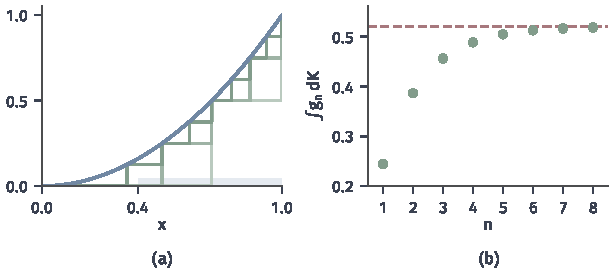
\includegraphics[width=104mm]{figures/07-probability/02-measure-theoretic-probability/matplotlib/cdis-simple-approx/figure.pdf}
  \caption{用简单函数逼近条件分布下的积分，三角形模型，$y=0.4$。(a)蓝线是$g(x)=x^{2}$，绿色阶梯是$g_n=2^{-n}\lfloor2^{n}g\rfloor$（$n=1,2,3$，颜色由浅到深），浅蓝区间$[0.4,1]$是$K(0.4,\cdot)$的支撑。(b)绿点是$\int g_n\,\mathrm{d}K(0.4,\cdot)$，$n=1,\dots,8$，红色虚线是极限$0.52$。}
  \label{fig:cdis-simple-approx}
\end{BookInlineFigure}

\paragraph{离散与密度的情形}
把定理~\ref{thm:cdis-integral-representation}用于前面的两类模型，就得到熟悉的公式。有概率表时，对$p_Y(y)>0$，
\[
 \mathbb{E}[g(X)\mid Y=y]=\sum_{x}g(x)\,\frac{p_{X,Y}(x,y)}{p_Y(y)} ;
\]
有联合密度时，由定理~\ref{thm:cdis-density-version}，对$0<f_Y(y)<\infty$，
\[
 \mathbb{E}[g(X)\mid Y=y]=\int g(x)\,\frac{f_{X,Y}(x,y)}{f_Y(y)}\,\mathrm{d}x .
\]
第~\ref{chap:random-vectors}章按这两个公式计算条件均值，当时它们只是“组内平均”的计算规则；现在可以说，它们给出的函数代入$Y$后正是条件期望的一个版本，第~\ref{chap:conditional-expectation}章关于条件期望的全部性质都可以用于它们。

三角形模型中，对$0\leq y<1$，
\[
 \mathbb{E}[g(X)\mid Y=y]=\frac{1}{1-y}\int_{y}^{1}g(x)\,\mathrm{d}x ,
\]
即$[y,1]$上$g$的平均值。取$g(x)=x$得到$(1+y)/2$，与第~\ref{chap:random-vectors}章的结果一致。

\subsection{条件矩的计算}
\label{sec:cdis-conditional-moments}

设$X$是实随机变量。取$g(x)=x^{k}$或$g(x)=\lvert x\rvert^{p}$，在相应的矩存在时，定理~\ref{thm:cdis-integral-representation}给出条件矩的积分公式：若$\mathbb{E}\lvert X\rvert^{p}<\infty$，$p>0$，则
\begin{equation}
 \mathbb{E}\bigl[\lvert X\rvert^{p}\bigm|Y\bigr]=\int\lvert x\rvert^{p}\,K(Y,\mathrm{d}x)<\infty\quad\text{几乎必然},
 \label{eq:cdis-conditional-abs-moment}
\end{equation}
若$k\leq p$是正整数，则几乎必然
\[
 \mathbb{E}[X^{k}\mid Y]=\int x^{k}\,K(Y,\mathrm{d}x),
\]
其中$\lvert x\rvert^{k}\leq1+\lvert x\rvert^{p}$保证$X^{k}$可积。这些量称为给定$Y$的\term{条件矩}（conditional moment）。

\paragraph{条件方差}
第~\ref{chap:conditional-expectation}章对$\mathbb{E}[X^{2}]<\infty$定义了条件方差
\[
 \operatorname{Var}(X\mid Y)=\mathbb{E}\bigl[(X-\mathbb{E}[X\mid Y])^{2}\bigm|Y\bigr].
\]
记$m(y)=\int x\,K(y,\mathrm{d}x)$，它在$P_Y$几乎每个$y$处有限，并且$m(Y)=\mathbb{E}[X\mid Y]$几乎必然。条件方差可以写成条件分布的方差。

\begin{theorem}[条件方差的积分表示]
\label{thm:cdis-conditional-variance}
设$\mathbb{E}[X^{2}]<\infty$，$K$是给定$Y$时$X$的正则条件分布。则几乎必然
\begin{equation}
 \operatorname{Var}(X\mid Y)=\int\bigl(x-m(Y)\bigr)^{2}\,K(Y,\mathrm{d}x)=\int x^{2}\,K(Y,\mathrm{d}x)-m(Y)^{2}.
 \label{eq:cdis-conditional-variance}
\end{equation}
\end{theorem}

\begin{proof}
由式~\eqref{eq:cdis-conditional-abs-moment}，存在$P_Y$零测集$N$，使$y\notin N$时$\int x^{2}\,K(y,\mathrm{d}x)<\infty$，从而$m(y)$有限。对这样的$y$，$K(y,\cdot)$是二阶矩有限的分布，展开平方得到
\[
 \begin{aligned}
 \int\bigl(x-m(y)\bigr)^{2}K(y,\mathrm{d}x)&=\int x^{2}K(y,\mathrm{d}x)-2m(y)^{2}+m(y)^{2}\\
 &=\int x^{2}K(y,\mathrm{d}x)-m(y)^{2}.
 \end{aligned}
\]
这是式~\eqref{eq:cdis-conditional-variance}的第二个等号。

另一方面，展开条件方差的定义。$m(Y)$与$X$都平方可积，由Cauchy--Schwarz不等式$m(Y)X$可积，于是可以用线性和提取已知量：
\[
 \begin{aligned}
 \operatorname{Var}(X\mid Y)&=\mathbb{E}[X^{2}\mid Y]-2m(Y)\,\mathbb{E}[X\mid Y]+m(Y)^{2}\\
 &=\mathbb{E}[X^{2}\mid Y]-m(Y)^{2}.
 \end{aligned}
\]
由式~\eqref{eq:cdis-conditional-abs-moment}取$p=2$，右边第一项$\mathbb{E}[X^{2}\mid Y]$几乎必然等于$\int x^{2}K(Y,\mathrm{d}x)$，两式相同。
\end{proof}

式~\eqref{eq:cdis-conditional-variance}就是“方差等于二阶矩减均值平方”对每个条件分布分别使用。它把条件方差从一个由积分刻画定义的随机变量，变成了每个观测值处一个具体分布的方差。

\paragraph{正面概率随机的硬币}
设$U\sim\operatorname{Unif}(0,1)$，给定$U=u$时把一枚正面概率为$u$的硬币独立地抛$n$次，$N$是正面次数。这句话本身就是用概率核描述的模型：
\[
 K(u,\{k\})=\binom{n}{k}u^{k}(1-u)^{n-k},\qquad k=0,1,\dots,n ,
\]
即给定$U=u$时$N\sim\operatorname{Bin}(n,u)$。联合规律由$U$的分布和这个核共同确定，第~\ref{sec:cdis-joint}节说明为什么这样确定的联合规律唯一，并且这个核就是它的正则条件分布。

二项分布的均值与方差在第~\ref{chap:common-distributions}章已经算出，代入式~\eqref{eq:cdis-integral-representation}与式~\eqref{eq:cdis-conditional-variance}，
\[
 \mathbb{E}[N\mid U]=nU,\qquad \operatorname{Var}(N\mid U)=nU(1-U).
\]
条件均值随$U$线性增长，条件方差在$U=\tfrac12$处最大，在两端趋于零。

由全方差公式，总方差是条件方差的平均加上条件均值的方差。用$\mathbb{E}[U]=\tfrac12$、$\mathbb{E}[U^{2}]=\tfrac13$、$\operatorname{Var}(U)=\tfrac1{12}$，
\[
 \mathbb{E}\bigl[nU(1-U)\bigr]=n\Bigl(\frac12-\frac13\Bigr)=\frac n6,\qquad \operatorname{Var}(nU)=\frac{n^{2}}{12}.
\]
于是
\[
 \operatorname{Var}(N)=\frac n6+\frac{n^{2}}{12}=\frac{n(n+2)}{12}.
\]
$n=10$时组内部分为$\tfrac53\approx1.67$，组间部分为$\tfrac{25}{3}\approx8.33$，总方差为$10$。组间部分随$n^{2}$增长，占了大头：抛得越多，正面次数的波动主要来自硬币本身的不确定，而不是给定硬币后的随机性。图~\ref{fig:cdis-coin-moments}画出这两部分。第~\ref{sec:cdis-mixture}小节将看到$N$在$\{0,1,\dots,n\}$上均匀分布，其方差$\bigl((n+1)^{2}-1\bigr)/12$与这里的结果相同。

\begin{BookInlineFigure}
  \centering
  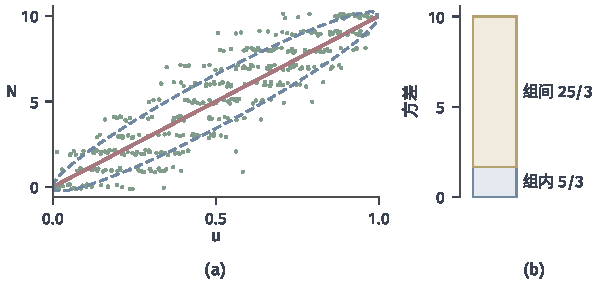
\includegraphics[width=104mm]{figures/07-probability/02-measure-theoretic-probability/matplotlib/cdis-coin-moments/figure.pdf}
  \caption{正面概率随机的硬币，$n=10$。(a)绿点是固定种子$3$模拟的$400$对$(U,N)$，纵向略加抖动以便看清；红线是条件均值$10u$，蓝色虚线是条件均值加减一个条件标准差$\sqrt{10u(1-u)}$。(b)总方差$10$的分解：浅蓝为组内部分$\tfrac53$，浅黄为组间部分$\tfrac{25}{3}$。}
  \label{fig:cdis-coin-moments}
\end{BookInlineFigure}

\paragraph{有限性只在几乎处处的意义下成立}
式~\eqref{eq:cdis-conditional-abs-moment}说整体矩有限保证条件矩\emph{几乎处处}有限，不能加强为对每个观测值有限。三角形模型中，把$y=\tfrac12$处的分布换成标准Cauchy分布，由第~\ref{sec:cdis-uniqueness}小节，所得的核仍是正则条件分布；可是Cauchy分布的绝对一阶矩是无穷，$\lvert x\rvert$关于$K'(\tfrac12,\cdot)$的积分发散，尽管$X$有界。哪个零测点上的条件矩有限，联合规律管不着。

反方向同样不成立：每个观测值上的条件矩有限，不能推出整体矩有限。设$Y\sim\operatorname{Unif}(0,1)$，给定$Y=y$时$X\sim\operatorname{Exp}(y)$，即率参数为$y$的指数分布。对每个$y\in(0,1)$，条件均值有限，
\[
 \int x\,K(y,\mathrm{d}x)=\frac1y<\infty .
\]
可是定理~\ref{thm:cdis-integral-representation}证明第三步中关于有限性的论证只用到简单函数与单调收敛，对任何非负$g$都成立，结果允许取$+\infty$：$\int(Kg)\,\mathrm{d}P_Y=\mathbb{E}[g(X)]$。取$g(x)=x$，
\[
 \mathbb{E}[X]=\int_0^1\frac1y\,\mathrm{d}y=+\infty .
\]
条件均值$1/y$在$y\to0$附近增长得太快，加权平均发散，见图~\ref{fig:cdis-moment-directions}。此时$X$不可积，第~\ref{chap:conditional-expectation}章的条件期望没有定义，只能说核的积分$1/y$是一个逐点有限的函数。

\begin{BookInlineFigure}
  \centering
  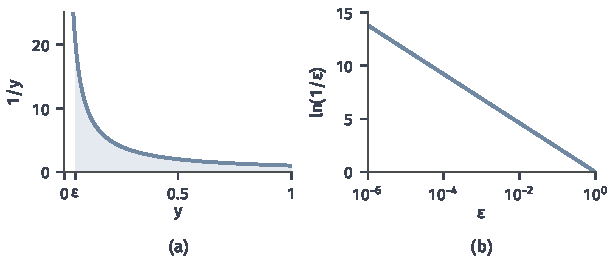
\includegraphics[width=104mm]{figures/07-probability/02-measure-theoretic-probability/matplotlib/cdis-moment-directions/figure.pdf}
  \caption{逐点有限的条件均值不保证整体可积。$Y\sim\operatorname{Unif}(0,1)$，给定$Y=y$时$X\sim\operatorname{Exp}(y)$。(a)蓝线是条件均值$1/y$，浅蓝区域是$[\varepsilon,1]$上的面积，$\varepsilon=0.05$。(b)蓝线是截断积分$\int_{\varepsilon}^{1}y^{-1}\,\mathrm{d}y=\ln(1/\varepsilon)$，横轴按对数刻度，$\varepsilon\to0$时无界增长。}
  \label{fig:cdis-moment-directions}
\end{BookInlineFigure}


\section{联合分布的分解}
\label{sec:cdis-joint}

上一节固定观测值，对条件分布积分。现在把观测值也放开，按观测的边缘分布再积分一次。概率表中，这相当于把条件分布的每一行乘回行的质量，恢复整张表；对列求和得到目标的边缘；逐个变量重复这一步，就能从头构造多个随机对象的联合规律。这一节依次落实这三件事，并说明每一步保留哪些条件变量。

\subsection{联合分布的恢复}
\label{sec:cdis-recovery}

引理~\ref{lem:cdis-regular-criterion}已经说明，矩形事件的联合概率可以由核与边缘恢复：
\[
 \mathbb{P}(X\in A,\ Y\in B)=\int_{B}K(y,A)\,P_Y(\mathrm{d}y).
\]
三角形模型中取$A=[\tfrac34,1]$、$B=[0,\tfrac12]$。对$y\leq\tfrac12$，$K(y,A)=\tfrac{1}{4(1-y)}$，乘以$f_Y(y)=2(1-y)$得到常数$\tfrac12$，所以
\[
 \mathbb{P}\bigl(X\geq\tfrac34,\ Y\leq\tfrac12\bigr)=\int_0^{1/2}\frac12\,\mathrm{d}y=\frac14 .
\]
直接计算，事件对应边长为$\tfrac14$与$\tfrac12$的矩形，它整个落在三角形内，面积$\tfrac18$乘以密度$2$也是$\tfrac14$，见图~\ref{fig:cdis-joint-recovery}。

\begin{BookInlineFigure}
  \centering
  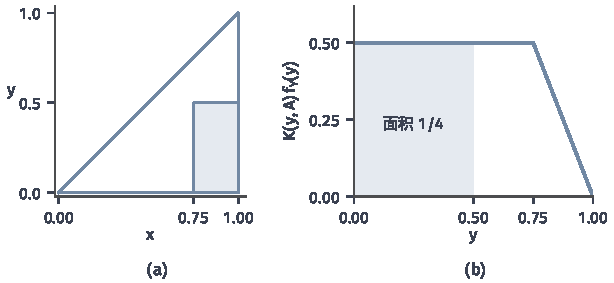
\includegraphics[width=104mm]{figures/07-probability/02-measure-theoretic-probability/matplotlib/cdis-joint-recovery/figure.pdf}
  \caption{由核与边缘恢复矩形事件的联合概率，三角形模型。(a)浅蓝矩形是事件$\{X\geq\tfrac34,\ Y\leq\tfrac12\}$，蓝线围成三角形。(b)蓝线是$y\mapsto K(y,A)f_Y(y)$，$A=[\tfrac34,1]$；它在$y\leq\tfrac34$时等于$\tfrac12$，此后等于$2(1-y)$。浅蓝区域是$[0,\tfrac12]$上的积分，面积为$\tfrac14$。}
  \label{fig:cdis-joint-recovery}
\end{BookInlineFigure}

矩形之外的事件，例如$\{X+Y\leq1\}$，以及一般的期望$\mathbb{E}[f(X,Y)]$，怎样由核与边缘算出？对乘积空间中的集合$E$，记它在$y$处的截面为$E^{y}=\{x:(x,y)\in E\}$。自然的猜测是先在每个$y$处按$K(y,\cdot)$量出截面，再按$Y$的分布累计。下面的定理说明这个猜测正确，并且由此定义的测度唯一。

\begin{theorem}[由核与边缘确定联合规律]
\label{thm:cdis-kernel-product}
设$\mu$是$\mathcal{Y}$上的概率测度，$K$是从$\mathcal{Y}$到$\mathcal{X}$的概率核。
\begin{enumerate}
 \item 对每个$E\in\mathcal{F}_{\mathcal{X}}\otimes\mathcal{F}_{\mathcal{Y}}$，$y\mapsto K(y,E^{y})$可测，并且
 \begin{equation}
  (\mu\otimes K)(E)=\int K(y,E^{y})\,\mu(\mathrm{d}y)
  \label{eq:cdis-kernel-product}
 \end{equation}
 是乘积空间上的概率测度。它是在每个可测矩形$A\times B$上取值$\int_{B}K(y,A)\,\mu(\mathrm{d}y)$的唯一概率测度。
 \item 对非负可测函数$f$，$y\mapsto\int f(x,y)\,K(y,\mathrm{d}x)$可测，并且
 \begin{equation}
  \int f\,\mathrm{d}(\mu\otimes K)=\int\!\!\int f(x,y)\,K(y,\mathrm{d}x)\,\mu(\mathrm{d}y).
  \label{eq:cdis-kernel-product-integral}
 \end{equation}
 若$f$关于$\mu\otimes K$可积，内层积分对$\mu$几乎每个$y$绝对收敛，式~\eqref{eq:cdis-kernel-product-integral}仍成立。
 \item 若$K$是给定$Y$时$X$的正则条件分布，则$P_Y\otimes K$就是$(X,Y)$的联合分布，从而对非负可测或使$f(X,Y)$可积的$f$，
 \begin{equation}
  \mathbb{E}[f(X,Y)]=\int\!\!\int f(x,y)\,K(y,\mathrm{d}x)\,P_Y(\mathrm{d}y).
  \label{eq:cdis-joint-recovery}
 \end{equation}
\end{enumerate}
\end{theorem}

\begin{proof}
第1条，先证可测性。令$\mathcal{D}$为使$y\mapsto K(y,E^{y})$可测的$E$的全体。对可测矩形，$(A\times B)^{y}$在$y\in B$时是$A$，否则是空集，所以$K(y,(A\times B)^{y})=K(y,A)\mathbf{1}_{B}(y)$可测，矩形属于$\mathcal{D}$。整个空间属于$\mathcal{D}$；补集的截面是截面的补集，$K(y,(E^{\mathrm{c}})^{y})=1-K(y,E^{y})$；两两不交的集合，截面也两两不交，$K(y,\cdot)$可数可加，所得的函数是可测函数之和。所以$\mathcal{D}$是$\lambda$系统。可测矩形对有限交封闭并生成乘积$\sigma$代数，由$\pi$--$\lambda$定理，$\mathcal{D}$包含全部可测集。

再证式~\eqref{eq:cdis-kernel-product}定义了概率测度。空集的截面都是空集，全空间的截面都是$\mathcal{X}$，所以测度分别为$0$和$1$。对两两不交的$E_n$，截面两两不交，
\[
 (\mu\otimes K)\Bigl(\bigcup_nE_n\Bigr)=\int\sum_{n}K(y,E_n^{y})\,\mu(\mathrm{d}y)=\sum_{n}(\mu\otimes K)(E_n),
\]
逐项积分的依据是单调收敛定理。取$E=A\times B$，式~\eqref{eq:cdis-kernel-product}给出$\int_{B}K(y,A)\,\mu(\mathrm{d}y)$。两个概率测度若在可测矩形上相同，由生成$\pi$系统上的唯一性，它们相同。

第2条，按积分的构造进行。$f=\mathbf{1}_{E}$时，内层积分是$K(y,E^{y})$，结论就是第1条。简单函数由线性得到。非负可测$f$取简单函数$f_n\uparrow f$：每个$y$处内层积分由单调收敛定理递增收敛，极限可测；外层再用一次单调收敛定理。$f$可积时，分别处理$f^{+}$与$f^{-}$；由非负情形，$\int\!\int\lvert f\rvert\,K(y,\mathrm{d}x)\,\mu(\mathrm{d}y)<\infty$，所以内层的$\int\lvert f(x,y)\rvert\,K(y,\mathrm{d}x)$只在$\mu$零测集上为无穷。

第3条，由引理~\ref{lem:cdis-regular-criterion}，$(X,Y)$的联合分布在每个可测矩形上的取值与$P_Y\otimes K$相同，由第1条的唯一性两者相同。式~\eqref{eq:cdis-joint-recovery}是第2条对联合分布的改写，其左边由分布的积分公式写成期望。
\end{proof}

定理与卷四的Tonelli、Fubini定理结构相同，可参考\BookChapterRef{chap:integration}{卷四第6章“积分”}。乘积测度是$K(y,\cdot)$不随$y$改变的特例：此时$\mu\otimes K$就是两个测度的乘积，$X$与$Y$独立。一般的核让截面的“量法”随$y$改变，这正是依赖关系的来源。

\paragraph{一个非矩形的例子}
用式~\eqref{eq:cdis-joint-recovery}计算三角形模型中的$\mathbb{E}[XY]$。内层对$x$积分时把$y$当作常数，由第~\ref{sec:cdis-integral-representation}小节，$\int x\,K(y,\mathrm{d}x)=(1+y)/2$，于是
\[
 \int x y\,K(y,\mathrm{d}x)=\frac{y(1+y)}{2}.
\]
再按$f_Y(y)=2(1-y)$积分，
\[
 \mathbb{E}[XY]=\int_0^1\frac{y(1+y)}{2}\cdot2(1-y)\,\mathrm{d}y=\int_0^1(y-y^{3})\,\mathrm{d}y=\frac14 .
\]
直接用联合密度计算，结果相同：
\[
 \int_0^1\int_0^{x}2xy\,\mathrm{d}y\,\mathrm{d}x=\int_0^1x^{3}\,\mathrm{d}x=\frac14 .
\]

\paragraph{给定观测时代入观测值}
定理~\ref{thm:cdis-kernel-product}还给出了一个常用的计算规则：求$f(X,Y)$给定$Y$的条件期望时，可以把$Y$的观测值代入，只对$X$按条件分布积分。设$\mathbb{E}\lvert f(X,Y)\rvert<\infty$，则
\begin{equation}
 \mathbb{E}[f(X,Y)\mid Y]=\int f(x,Y)\,K(Y,\mathrm{d}x)\quad\text{几乎必然}.
 \label{eq:cdis-substitution}
\end{equation}
右边由第2条是$Y$的可测函数。对$B\in\mathcal{F}_{\mathcal{Y}}$，把式~\eqref{eq:cdis-joint-recovery}用于$\mathbf{1}_{B}(y)f(x,y)$，得到右边在$\{Y\in B\}$上的积分等于$\mathbb{E}[\mathbf{1}_{\{Y\in B\}}f(X,Y)]$，这正是条件期望的积分刻画。例如$\mathbb{E}[XY\mid Y]=Y\,\mathbb{E}[X\mid Y]$，与提取已知量的规则一致。

\paragraph{不只是密度的乘法}
有联合密度时，式~\eqref{eq:cdis-joint-recovery}就是在$f_Y(y)>0$处把$f_{X,Y}$写成$f_Y(y)f_{X\mid Y}(x\mid y)$再作累次积分。定理本身不需要密度。图~\ref{fig:cdis-non-density}给出两个没有平面联合密度的例子。

\begin{BookInlineFigure}
  \centering
  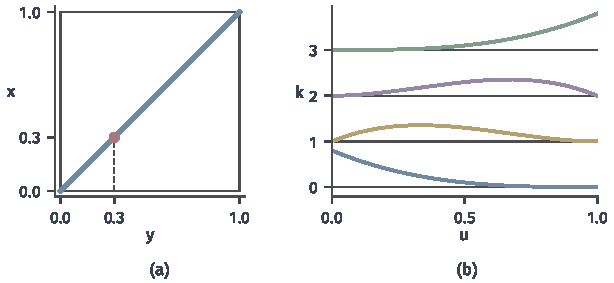
\includegraphics[width=104mm]{figures/07-probability/02-measure-theoretic-probability/matplotlib/cdis-non-density/figure.pdf}
  \caption{由核与边缘确定、但没有平面联合密度的联合规律。(a)$X=Y\sim\operatorname{Unif}(0,1)$：全部质量在蓝色对角线上，核$K(y,\cdot)=\delta_y$把$y=0.3$处的质量放在红点。(b)正面概率随机的硬币，$n=3$：$(U,N)$的质量分布在四条水平线$N=k$上，曲线是每条线上的密度$\binom{3}{k}u^{k}(1-u)^{3-k}$，$k=0,1,2,3$（蓝、黄、紫、绿）。}
  \label{fig:cdis-non-density}
\end{BookInlineFigure}

第一个例子是$X=Y\sim\operatorname{Unif}(0,1)$，核为$K(y,\cdot)=\delta_y$。由式~\eqref{eq:cdis-kernel-product}，$E^{y}$在$\delta_y$下的测度是$\mathbf{1}_{E}(y,y)$，所以
\[
 P_{(X,Y)}(E)=\int_0^1\mathbf{1}_{E}(y,y)\,\mathrm{d}y ,
\]
即质量沿对角线均匀分布。例如取$f(x,y)=(x-y)^{2}$，内层积分在每个$y$处都是$0$，所以$\mathbb{E}[(X-Y)^{2}]=0$。

第二个例子是硬币模型$(U,N)$，一个分量连续、一个分量离散。$N=k$的那条水平线上，质量关于$u$的密度是$\binom nk u^{k}(1-u)^{n-k}$；所有线上的密度对$u$积分再对$k$求和等于$1$。这两种联合规律都不是平面上的密度，却都由“边缘乘以核”唯一确定。

\subsection{全概率公式与混合分布}
\label{sec:cdis-mixture}

联合恢复公式中取$B=\mathcal{Y}$，即保留$X$的事件、对全部观测值积分，得到$X$的边缘分布：
\begin{equation}
 P_X(A)=\int K(y,A)\,P_Y(\mathrm{d}y),\qquad A\in\mathcal{F}_{\mathcal{X}} .
 \label{eq:cdis-total-probability}
\end{equation}
这是全概率公式的一般形式。第~\ref{chap:classical-probability}章的全概率公式把样本空间分成有限个正概率的组，再按组加权；这里的“组”是观测值$y$，可以有不可数多个，每组的概率可以为零，按$P_Y$加权的求和换成了积分。对函数，同样有$\mathbb{E}[g(X)]=\int(Kg)(y)\,P_Y(\mathrm{d}y)$，只要$g$非负或$g(X)$可积。

式~\eqref{eq:cdis-total-probability}也可以从另一个方向读：给定一族分布$\{K(y,\cdot)\}$和一个加权分布$\mu$，$\mu K$是一个新分布，称为这族分布按$\mu$的混合。$\mu$称为混合分布的权重，取值$y$称为混合变量。第~\ref{chap:random-vectors}章的房间温度模型就是两个分量的离散混合：$Y$表示房间状态，$\mu$给两种状态的概率$0.8$与$0.2$，$K$给出两个高斯分布，混合结果的密度是$0.8\,\phi(x-20)+0.2\,\phi(x-23)$。

\paragraph{连续混合：随机硬币的正面次数}
混合变量可以连续。硬币模型中，$U$的分布是$[0,1]$上的Lebesgue测度，代入式~\eqref{eq:cdis-total-probability}，
\[
 \mathbb{P}(N=k)=\int_0^1\binom nk u^{k}(1-u)^{n-k}\,\mathrm{d}u .
\]
由第~\ref{chap:common-distributions}章的Beta积分，对非负整数$a,b$，
\[
 \int_0^1u^{a}(1-u)^{b}\,\mathrm{d}u=\frac{a!\,b!}{(a+b+1)!},
\]
代入得到
\[
 \mathbb{P}(N=k)=\frac{n!}{k!\,(n-k)!}\cdot\frac{k!\,(n-k)!}{(n+1)!}=\frac{1}{n+1},\qquad k=0,1,\dots,n .
\]
正面次数在$\{0,1,\dots,n\}$上均匀分布。每个分量$\operatorname{Bin}(n,u)$都集中在$nu$附近，$u$均匀地扫过$[0,1]$，峰的位置也均匀地扫过$0$到$n$，叠加起来恰好铺平，见图~\ref{fig:cdis-mixtures}(a)。

\paragraph{连续混合：正态尺度混合}
第~\ref{chap:multivariate-distributions}章的多元t分布是另一个连续混合。那里$U\sim\chi^{2}_{\nu}$，给定$U=u$时$\bm{X}\sim\mathcal{N}\bigl(\bm{\mu},(\nu/u)\bm{\Sigma}\bigr)$，即核$K(u,\cdot)$是一族尺度不同的高斯分布。式~\eqref{eq:cdis-total-probability}给出
\[
 P_{\bm{X}}(S)=\int_0^{\infty}K(u,S)\,P_U(\mathrm{d}u),
\]
再对每个$K(u,\cdot)$的密度$g_u$用Tonelli定理交换积分，就得到那一章的混合密度：$\bm{X}$的密度是各分量密度$g_u(\bm{x})$按$P_U$的加权积分。这里的推导不需要$U$有密度：把尺度的分布换成任何$(0,\infty)$上的分布，例如只取两个值，混合仍有密度，只要每个分量有密度且$u\mapsto g_u(\bm{x})$可测。

\begin{BookInlineFigure}
  \centering
  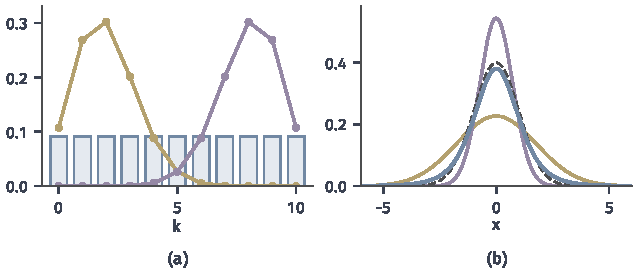
\includegraphics[width=108mm]{figures/07-probability/02-measure-theoretic-probability/matplotlib/cdis-mixtures/figure.pdf}
  \caption{两个连续混合。(a)$n=10$时的两个分量$\operatorname{Bin}(10,u)$，$u=0.2$（黄）与$u=0.8$（紫），以及对$u\in[0,1]$均匀混合后的分布，各点概率都是$1/11$（浅蓝柱）。(b)一元t分布作为正态尺度混合，$\nu=5$：黄、紫线是$U$取$\chi^{2}_{5}$的$10\%$与$90\%$分位数时的分量$\mathcal{N}(0,5/u)$，蓝线是混合得到的t密度，灰色虚线是$\mathcal{N}(0,1)$。}
  \label{fig:cdis-mixtures}
\end{BookInlineFigure}

图~\ref{fig:cdis-mixtures}(b)中，$u$较小的分量又宽又矮，$u$较大的分量窄而高；混合后的t密度中心比标准高斯略低，尾部明显更厚，厚尾来自那些尺度很大的分量。混合分布的矩也按条件矩加权：均值是条件均值的平均，方差由全方差公式分成组内与组间两部分，第~\ref{sec:cdis-conditional-moments}小节的硬币例子就是一次具体的计算。

\subsection{链式分解}
\label{sec:cdis-chain}

两个随机对象的联合规律可以分成“先$Y$、再给定$Y$的$X$”两步。有$n$个随机对象$X_1,\dots,X_n$时，可以依次进行：先定$X_1$，再给定$X_1$定$X_2$，再给定$(X_1,X_2)$定$X_3$，如此下去。每一步需要一个正则条件分布，它的存在由定理~\ref{thm:cdis-existence}保证，这里要求每个$X_k$取值于标准Borel空间$\mathcal{X}_k$。

记$\bm{x}_{1:k}=(x_1,\dots,x_k)$，$X_{1:k}=(X_1,\dots,X_k)$。下面的定理用到一个事实：标准Borel空间的有限乘积仍是标准Borel空间，这是第~\ref{sec:cdis-existence-conditions}小节所述可数乘积结论的特例。

\begin{theorem}[链式分解]
\label{thm:cdis-chain}
设$X_1,\dots,X_n$分别取值于标准Borel空间$\mathcal{X}_1,\dots,\mathcal{X}_n$。则存在概率核$K_k$（$k=2,\dots,n$），$K_k$从$\mathcal{X}_1\times\cdots\times\mathcal{X}_{k-1}$到$\mathcal{X}_k$，是给定$X_{1:k-1}$时$X_k$的正则条件分布；并且对非负可测函数$f$，
\begin{equation}
 \mathbb{E}[f(X_{1:n})]=\int P_{X_1}(\mathrm{d}x_1)\int K_2(x_1,\mathrm{d}x_2)\cdots\int K_n(\bm{x}_{1:n-1},\mathrm{d}x_n)\,f(\bm{x}_{1:n}).
 \label{eq:cdis-chain}
\end{equation}
反过来，任给$\mathcal{X}_1$上的概率测度$P_1$和这样的一列概率核$K_2,\dots,K_n$，式~\eqref{eq:cdis-chain}的右边（取$f$为指示函数）定义了乘积空间上唯一的概率测度；在这个测度下，坐标$X_1$的分布是$P_1$，$K_k$是给定$X_{1:k-1}$时$X_k$的正则条件分布。
\end{theorem}

\begin{proof}
对$n$归纳。$n=1$时式~\eqref{eq:cdis-chain}是分布的积分公式。设结论对$n-1$成立。$X_{1:n-1}$取值于标准Borel空间$\mathcal{X}_1\times\cdots\times\mathcal{X}_{n-1}$，由定理~\ref{thm:cdis-existence}，给定$X_{1:n-1}$时$X_n$的正则条件分布$K_n$存在。由定理~\ref{thm:cdis-kernel-product}第3条，取$Y=X_{1:n-1}$、$X=X_n$，
\[
 \mathbb{E}[f(X_{1:n})]=\int\Bigl(\int f(\bm{x}_{1:n-1},x_n)\,K_n(\bm{x}_{1:n-1},\mathrm{d}x_n)\Bigr)P_{X_{1:n-1}}(\mathrm{d}\bm{x}_{1:n-1}).
\]
括号内是$\bm{x}_{1:n-1}$的非负可测函数，对它用归纳假设展开外层积分，就得到式~\eqref{eq:cdis-chain}。

反方向同样归纳：由$P_1$与$K_2$，定理~\ref{thm:cdis-kernel-product}第1条给出$\mathcal{X}_1\times\mathcal{X}_2$上唯一的测度$\mu_2=P_1\otimes K_2$；再由$\mu_2$与$K_3$得到$\mu_3=\mu_2\otimes K_3$，依此类推。每一步的唯一性来自第1条。在$\mu_k$下，由第1条中的矩形公式与引理~\ref{lem:cdis-regular-criterion}，$K_k$是给定前$k-1$个坐标时第$k$个坐标的正则条件分布；后面各步只在前$k$个坐标之外添加新坐标，不改变前$k$个坐标的联合分布。
\end{proof}

正向的结论说，任何有限个标准Borel随机对象的联合规律都能逐次分解；反向的结论说，可以用起始分布和一列核逐步构造联合规律：先按$P_1$抽$x_1$，再按$K_2(x_1,\cdot)$抽$x_2$，再按$K_3(x_1,x_2,\cdot)$抽$x_3$。每一步的核都可以依赖已经得到的\emph{全部}取值。按这种方式实际产生样本的方法在第~\ref{chap:sample-generation}章研究。有联合密度时，式~\eqref{eq:cdis-chain}就是密度的连乘分解
\[
 f(\bm{x}_{1:n})=f_{X_1}(x_1)\,f_{X_2\mid X_1}(x_2\mid x_1)\cdots f_{X_n\mid X_{1:n-1}}(x_n\mid\bm{x}_{1:n-1}),
\]
在各边缘密度为正的范围内成立。

\paragraph{随机硬币的逐次抛掷}
回到正面概率为$U\sim\operatorname{Unif}(0,1)$的硬币，记第$k$次的结果为$X_k\in\{0,1\}$，$1$表示正面，给定$U=u$时各次独立且$\mathbb{P}(X_k=1\mid U=u)=u$。前$m$次中正面有$s$次的某个具体结果序列，概率是
\[
 \mathbb{P}(X_{1:m}=\bm{x}_{1:m})=\int_0^1u^{s}(1-u)^{m-s}\,\mathrm{d}u=\frac{s!\,(m-s)!}{(m+1)!}.
\]
它只依赖正面次数$s$，与正反面出现的次序无关。

给定前$k-1$次的结果，其中正面$s$次，第$k$次为正面的条件概率是两个这样的概率之比，取$m=k-1$：
\begin{equation}
 \mathbb{P}(X_k=1\mid X_{1:k-1}=\bm{x}_{1:k-1})=\frac{(s+1)!\,(k-1-s)!/(k+1)!}{s!\,(k-1-s)!/k!}=\frac{s+1}{k+1}.
 \label{eq:cdis-succession}
\end{equation}
这称为\term{Laplace继承法则}（Laplace's rule of succession）。先看到的正面越多，下一次越可能是正面：抛掷结果在不断透露$U$的信息。由于每个$\bm{x}_{1:k-1}$的概率为正，这里的核由初等条件概率唯一确定。

用链式分解计算$\mathbb{P}(X_1=1,X_2=1,X_3=0)$。三个因子依次由式~\eqref{eq:cdis-succession}取$k=1,2,3$得到：
\[
 \begin{gathered}
 \mathbb{P}(X_1=1)=\frac12,\qquad \mathbb{P}(X_2=1\mid X_1=1)=\frac23,\\
 \mathbb{P}(X_3=0\mid X_1=1,X_2=1)=1-\frac34=\frac14 .
 \end{gathered}
\]
相乘得到$\tfrac1{12}$，与直接积分的结果相同：
\[
 \int_0^1u^{2}(1-u)\,\mathrm{d}u=\frac13-\frac14=\frac1{12}.
\]
图~\ref{fig:cdis-succession-tree}画出全部八条路径。

\begin{BookInlineFigure}
  \centering
  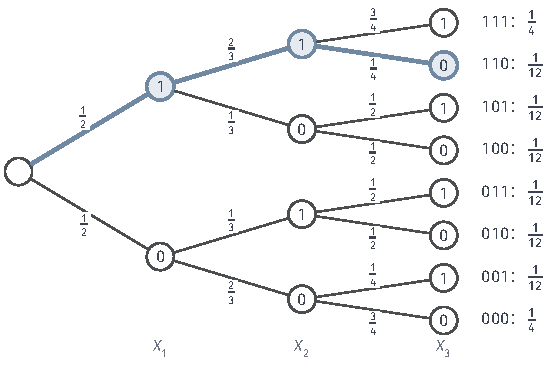
\includegraphics[width=94mm]{figures/07-probability/02-measure-theoretic-probability/tikz/cdis-succession-tree/figure.pdf}
  \caption{随机硬币前三次抛掷的链式分解。每条边上是由Laplace继承法则得到的条件概率，右侧是八个结果序列的概率；蓝色路径是$(1,1,0)$，概率为$\tfrac12\cdot\tfrac23\cdot\tfrac14=\tfrac1{12}$。}
  \label{fig:cdis-succession-tree}
\end{BookInlineFigure}

\paragraph{省去条件变量的后果}
式~\eqref{eq:cdis-chain}中每个核都给定了此前的全部变量。若为了简便，第三步只用$X_2$而忽略$X_1$，计算会出错。三次抛掷的联合规律在交换次序后不变，所以$(X_2,X_3)$与$(X_1,X_2)$同分布，
\[
 \mathbb{P}(X_3=0\mid X_2=1)=\mathbb{P}(X_2=0\mid X_1=1)=\frac13 ,
\]
于是“省略版”给出
\[
 \frac12\cdot\frac23\cdot\frac13=\frac19\neq\frac1{12}.
\]
差别的来源是：$X_1=1$与$X_2=1$合起来比单独的$X_2=1$透露了更多关于$U$的信息，使下一次出现反面的可能更小。图~\ref{fig:cdis-chain-omit}比较了八个序列在两种算法下的概率。省略版仍然给出一个总和为$1$的分布，所以无法从归一性看出错误。

\begin{BookInlineFigure}
  \centering
  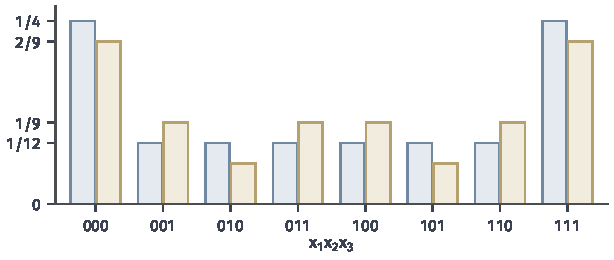
\includegraphics[width=104mm]{figures/07-probability/02-measure-theoretic-probability/matplotlib/cdis-chain-omit/figure.pdf}
  \caption{随机硬币三次抛掷的八个结果序列。蓝柱是由完整链式分解得到的真实概率，黄柱是第三步只给定$X_2$时的“省略版”概率；两组各自的和都是$1$，但在每个序列上都不相同。}
  \label{fig:cdis-chain-omit}
\end{BookInlineFigure}

一般地，把$K_k(\bm{x}_{1:k-1},\cdot)$换成只依赖其中一部分变量的核，是一个需要证明的断言：给定那部分变量以后，被省去的变量对$X_k$不再提供信息。这正是下一节的条件独立。


\section{条件独立}
\label{sec:cdis-conditional-independence}

上一节的硬币例子里，三次抛掷互不独立，可是一旦知道$U$，它们就是独立的抛掷：给定$U$以后，联合规律拆成了各次条件分布的乘积。什么时候给定一份信息以后，两个随机对象的联合规律可以这样拆开？拆开以后，链式分解中哪些条件变量可以省去？这一节先给出定义和判别，再看改变条件信息会怎样影响独立关系，最后用条件独立化简核的复合。

设$X,Z$分别取值于$(\mathcal{X},\mathcal{F}_{\mathcal{X}})$与$(\mathcal{Z},\mathcal{F}_{\mathcal{Z}})$，$\mathcal{G}$是子$\sigma$代数。

\subsection{定义与乘积分解}
\label{sec:cdis-ci-definition}

独立可以写成期望的乘积分解：对有界可测的$f,g$，
\[
 \mathbb{E}[f(X)g(Z)]=\mathbb{E}[f(X)]\,\mathbb{E}[g(Z)].
\]
把期望换成给定$\mathcal{G}$的条件期望，就得到给定信息后的版本。

\begin{definition}[条件独立]
\label{def:cdis-conditional-independence}
若对任意有界可测函数$f:\mathcal{X}\to\mathbb{R}$与$g:\mathcal{Z}\to\mathbb{R}$，
\begin{equation}
 \mathbb{E}[f(X)g(Z)\mid\mathcal{G}]=\mathbb{E}[f(X)\mid\mathcal{G}]\,\mathbb{E}[g(Z)\mid\mathcal{G}]\quad\text{几乎必然},
 \label{eq:cdis-conditional-independence}
\end{equation}
则称$X$与$Z$在给定$\mathcal{G}$时\term{条件独立}（conditionally independent），记作$X\perp\!\!\!\perp Z\mid\mathcal{G}$。$\mathcal{G}=\sigma(Y)$时记作$X\perp\!\!\!\perp Z\mid Y$。
\end{definition}

取$f=\mathbf{1}_{A}$、$g=\mathbf{1}_{C}$，定义包含了事件形式
\[
 \mathbb{P}(X\in A,\ Z\in C\mid\mathcal{G})=\mathbb{P}(X\in A\mid\mathcal{G})\,\mathbb{P}(Z\in C\mid\mathcal{G})\quad\text{几乎必然}.
\]
反过来，事件形式对一切$A,C$成立时，两边对$f,g$都是线性的，所以对简单函数成立；有界可测函数是简单函数的一致极限，而有界函数$h$的条件期望的绝对值几乎必然不超过$\sup\lvert h\rvert$，取极限即得式~\eqref{eq:cdis-conditional-independence}。$\mathcal{G}$只含零概率与全概率事件时，条件期望就是期望，条件独立回到独立。

\paragraph{条件联合分布的乘积}
给定观测$Y$、且$(X,Z)$有正则条件分布时，定义可以在每个观测值处读出来。设$\mathcal{X},\mathcal{Z}$都是标准Borel空间，$K$是给定$Y$时$(X,Z)$的正则条件分布。令
\[
 K_X(y,A)=K(y,A\times\mathcal{Z}),\qquad K_Z(y,C)=K(y,\mathcal{X}\times C),
\]
它们是$K(y,\cdot)$的两个边缘，并且分别是给定$Y$时$X$与$Z$的正则条件分布。例如，几乎必然有
\[
 K_X(Y,A)=\mathbb{P}\bigl((X,Z)\in A\times\mathcal{Z}\bigm|Y\bigr)=\mathbb{P}(X\in A\mid Y).
\]

\begin{theorem}[条件独立的乘积判别]
\label{thm:cdis-ci-product}
在上述设定下，$X\perp\!\!\!\perp Z\mid Y$当且仅当对$P_Y$几乎每个$y$，
\begin{equation}
 K(y,\cdot)=K_X(y,\cdot)\otimes K_Z(y,\cdot),
 \label{eq:cdis-ci-product}
\end{equation}
即给定$Y=y$时，$(X,Z)$的条件分布是两个条件边缘的乘积测度。
\end{theorem}

\begin{proof}
设式~\eqref{eq:cdis-ci-product}在$P_Y$零测集$N$之外成立。对任意$A,C$，在$\{Y\notin N\}$上$K(Y,A\times C)=K_X(Y,A)K_Z(Y,C)$，三个核都是相应条件概率的版本，所以事件形式几乎必然成立，从而$X\perp\!\!\!\perp Z\mid Y$。

反过来设$X\perp\!\!\!\perp Z\mid Y$。如定理~\ref{thm:cdis-uniqueness}的证明，取生成$\mathcal{F}_{\mathcal{X}}$与$\mathcal{F}_{\mathcal{Z}}$的可数$\pi$系统$\mathcal{P}_X$、$\mathcal{P}_Z$。对$A\in\mathcal{P}_X$、$C\in\mathcal{P}_Z$，由事件形式，
\[
 \begin{aligned}
 K(Y,A\times C)&=\mathbb{P}(X\in A,\ Z\in C\mid Y)\\
 &=\mathbb{P}(X\in A\mid Y)\,\mathbb{P}(Z\in C\mid Y)=K_X(Y,A)\,K_Z(Y,C)
 \end{aligned}
\]
几乎必然成立。这是可数个关系，例外集的并$N$满足$P_Y(N)=0$。对$y\notin N$，两个概率测度$K(y,\cdot)$与$K_X(y,\cdot)\otimes K_Z(y,\cdot)$在矩形族$\{A\times C:A\in\mathcal{P}_X,\ C\in\mathcal{P}_Z\}$上相同；这个族可数、对有限交封闭，并生成乘积$\sigma$代数，所以两个测度相同。
\end{proof}

有概率表时，式~\eqref{eq:cdis-ci-product}就是说：对每个正概率的观测值$y$，给定$Y=y$的条件概率表$p(x,z\mid y)$是它的行和与列和之积。这是第~\ref{chap:random-vectors}章独立判别的逐层版本，每个$y$对应一层表。

\paragraph{用一个变量的条件分布判别}
链式分解需要的是另一种等价形式：已经知道$Y$以后，再知道$X$不改变$Z$的条件分布。

\begin{theorem}[条件独立与条件变量的省略]
\label{thm:cdis-ci-markov}
$X\perp\!\!\!\perp Z\mid Y$当且仅当对每个$C\in\mathcal{F}_{\mathcal{Z}}$，
\begin{equation}
 \mathbb{P}(Z\in C\mid X,Y)=\mathbb{P}(Z\in C\mid Y)\quad\text{几乎必然}.
 \label{eq:cdis-ci-markov}
\end{equation}
\end{theorem}

\begin{proof}
设$X\perp\!\!\!\perp Z\mid Y$，固定$C$，令$W=\mathbb{P}(Z\in C\mid Y)$。$W$是$\sigma(Y)$可测的，当然也是$\sigma(X,Y)$可测的。要证$W$满足给定$\sigma(X,Y)$的条件期望的积分刻画，先对形如$\{X\in A,\ Y\in B\}$的事件核对。利用全期望公式、条件独立与提取已知量，
\[
 \begin{aligned}
 &\mathbb{E}\bigl[\mathbf{1}_{\{X\in A\}}\mathbf{1}_{\{Y\in B\}}\mathbf{1}_{\{Z\in C\}}\bigr]\\
 &\qquad=\mathbb{E}\bigl[\mathbf{1}_{\{Y\in B\}}\,\mathbb{P}(X\in A,\ Z\in C\mid Y)\bigr]\\
 &\qquad=\mathbb{E}\bigl[\mathbf{1}_{\{Y\in B\}}\,\mathbb{P}(X\in A\mid Y)\,W\bigr]\\
 &\qquad=\mathbb{E}\bigl[\mathbf{1}_{\{X\in A\}}\mathbf{1}_{\{Y\in B\}}\,W\bigr].
 \end{aligned}
\]
最后一步把$\mathbf{1}_{\{Y\in B\}}W$当作已知量，对$\mathbf{1}_{\{X\in A\}}$用全期望公式反向展开。这些事件对有限交封闭并生成$\sigma(X,Y)$；使积分等式成立的事件全体对补集和不交可数并封闭，是$\lambda$系统，由$\pi$--$\lambda$定理包含$\sigma(X,Y)$。所以$W=\mathbb{P}(Z\in C\mid X,Y)$几乎必然。

反过来设式~\eqref{eq:cdis-ci-markov}成立。由塔式法则、提取已知量与式~\eqref{eq:cdis-ci-markov}，
\[
 \begin{aligned}
 \mathbb{P}(X\in A,\ Z\in C\mid Y)
 &=\mathbb{E}\bigl[\mathbf{1}_{\{X\in A\}}\,\mathbb{P}(Z\in C\mid X,Y)\bigm|Y\bigr]\\
 &=\mathbb{E}\bigl[\mathbf{1}_{\{X\in A\}}\,\mathbb{P}(Z\in C\mid Y)\bigm|Y\bigr]\\
 &=\mathbb{P}(X\in A\mid Y)\,\mathbb{P}(Z\in C\mid Y),
 \end{aligned}
\]
这是事件形式的条件独立。
\end{proof}

用核来说：若$X\perp\!\!\!\perp Z\mid Y$，给定$(X,Y)$时$Z$的正则条件分布可以取成只依赖$y$的核$K_Z(y,\cdot)$；链式分解中$Z$那一步的条件变量$X$就可以省去。上一节的硬币例子中，给定$U$时各次抛掷条件独立，所以给定$(U,X_1,X_2)$时$X_3$的条件分布只依赖$U$；可是不给$U$时，省去$X_1$并不合法。

\paragraph{条件协方差为零并不足够}
条件独立要求对所有有界函数分解，只检查条件协方差为零不够，这里条件协方差指
\[
 \operatorname{Cov}(X,Z\mid Y)=\mathbb{E}[XZ\mid Y]-\mathbb{E}[X\mid Y]\,\mathbb{E}[Z\mid Y].
\]
设$X$在$\{-1,0,1\}$上均匀分布并与$Y$独立，$Z=X^{2}$。对每个$y$，给定$Y=y$时$X$仍在$\{-1,0,1\}$上均匀，于是
\[
 \operatorname{Cov}(X,Z\mid Y)=\mathbb{E}[X^{3}]-\mathbb{E}[X]\,\mathbb{E}[X^{2}]=0-0\cdot\tfrac23=0 .
\]
可是
\[
 \mathbb{P}(X=0,\ Z=1\mid Y)=0\neq\tfrac13\cdot\tfrac23=\mathbb{P}(X=0\mid Y)\,\mathbb{P}(Z=1\mid Y),
\]
$Z$是$X$的函数，二者完全不独立。这与第~\ref{chap:random-vectors}章“不相关不推出独立”是同一件事，只是在每个观测值上分别发生。

\subsection{条件信息的影响}
\label{sec:cdis-ci-information}

独立与条件独立之间没有一般的蕴含关系，增加或减少条件信息都可能改变独立性。下面两个例子各说明一个方向。

\paragraph{独立但不条件独立}
设$X_1,X_2$是两枚独立的公平硬币，$1$表示正面，$S=X_1+X_2$。无条件时，四种结果各占$\tfrac14$，$X_1$与$X_2$独立。给定$S=1$，只剩$(1,0)$与$(0,1)$两种结果，各占一半：
\[
 \begin{gathered}
 \mathbb{P}(X_1=1,\ X_2=1\mid S=1)=0,\\
 \mathbb{P}(X_1=1\mid S=1)\,\mathbb{P}(X_2=1\mid S=1)=\tfrac12\cdot\tfrac12=\tfrac14 .
 \end{gathered}
\]
$\mathbb{P}(S=1)=\tfrac12>0$，这个失败不在零测集上，所以$X_1$与$X_2$给定$S$时不条件独立。原因在图~\ref{fig:cdis-ci-tables}(a)中可以看出：条件化取出的是一条反对角线，知道和以后，一枚硬币的结果完全确定了另一枚。

\begin{BookInlineFigure}
  \centering
  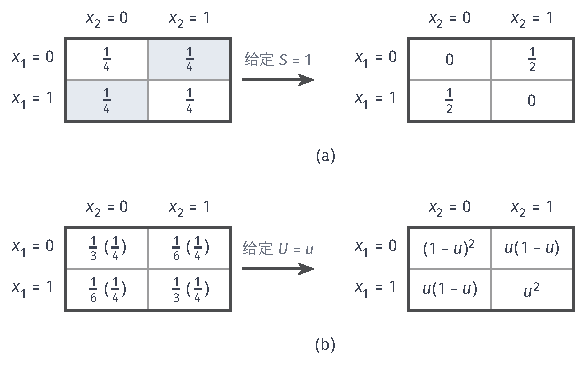
\includegraphics[width=98mm]{figures/07-probability/02-measure-theoretic-probability/tikz/cdis-ci-tables/figure.pdf}
  \caption{独立性随条件信息改变。(a)两枚独立公平硬币的联合概率表，浅蓝格子是事件$\{S=1\}$；给定$S=1$后只剩反对角线上的两格，$X_1$决定$X_2$。(b)随机硬币前两次抛掷的联合概率表，与各格边缘乘积（括号内）对照；给定$U=u$时表变为$u,1-u$的乘积表（右侧），条件独立而无条件不独立。}
  \label{fig:cdis-ci-tables}
\end{BookInlineFigure}

\paragraph{条件独立但不独立}
反方向用随机硬币。给定$U=u$时$X_1,X_2$独立，各以概率$u$为正面，所以$X_1\perp\!\!\!\perp X_2\mid U$。不给$U$时，由第~\ref{sec:cdis-chain}小节的公式，
\[
 \mathbb{P}(X_1=1,\ X_2=1)=\int_0^1u^{2}\,\mathrm{d}u=\frac13\neq\frac14=\mathbb{P}(X_1=1)\,\mathbb{P}(X_2=1).
\]
二者正相关，协方差为$\tfrac13-\tfrac14=\tfrac1{12}$，恰好是$\operatorname{Var}(U)$：两次抛掷共用同一个未知的正面概率，第一次的结果透露了$U$，于是影响对第二次的判断。

两个例子放在一起看。第一个例子中，$S$由$X_1,X_2$共同决定；把它加入条件，原本独立的两个量变得相关。第二个例子中，$U$同时影响$X_1,X_2$；把它从条件中去掉，原本条件独立的两个量变得相关。增加信息并不总是破坏独立：第二个例子中再给定$X_3$，即给定$(U,X_3)$，$X_1$与$X_2$仍然条件独立，因为给定$U$时三次抛掷相互独立。条件独立是$X$、$Z$与所给信息三者共同的性质，换了信息就要重新检查。

\paragraph{条件化与干预}
条件化回答的是“观测到$X_1=1$以后，对$X_2$的判断应当怎样修正”。随机硬币中，答案是把$\mathbb{P}(X_2=1)$从$\tfrac12$改成$\tfrac23$。另一个问题是：若有人不抛第一枚硬币，而是直接把它的记录写成正面，第二次抛掷的规律会怎样？这时硬币的正面概率$U$没有受到任何影响，第二次仍以$\tfrac12$的概率出现正面。

这两个问题的答案不同，而且第二个问题不能只靠联合分布回答。另一个模型是：第一次是公平硬币，第二次在第一次为正面时以$\tfrac23$、为反面时以$\tfrac13$出现正面。它与随机硬币的$(X_1,X_2)$有完全相同的联合分布，但在这个模型里改写第一次的记录，第二次正面的概率会变成$\tfrac23$。条件概率由联合规律决定；改变某个变量的产生方式以后会发生什么，还依赖产生数据的机制。研究这种操作的模型可参考\BookChapterRef{chap:causal-models-counterfactuals}{卷八第10章“因果模型与反事实”}。

\subsection{条件独立下的核复合}
\label{sec:cdis-composition}

设$X,Y,Z$都取值于标准Borel空间。已知给定$X$时$Y$的条件分布$K_{Y\mid X}$，以及给定$Y$时$Z$的条件分布$K_{Z\mid Y}$，能否得到给定$X$时$Z$的条件分布？一个自然的公式是先按$K_{Y\mid X}(x,\cdot)$抽出中间值$y$，再按$K_{Z\mid Y}(y,\cdot)$抽$z$，即对中间值积分。这个公式需要条件独立。

\begin{theorem}[核的复合]
\label{thm:cdis-composition}
设$X\perp\!\!\!\perp Z\mid Y$，$K_{Y\mid X}$与$K_{Z\mid Y}$分别是给定$X$时$Y$、给定$Y$时$Z$的正则条件分布。则
\begin{equation}
 L(x,C)=\int K_{Z\mid Y}(y,C)\,K_{Y\mid X}(x,\mathrm{d}y)
 \label{eq:cdis-composition}
\end{equation}
是给定$X$时$Z$的正则条件分布。
\end{theorem}

\begin{proof}
先说明$L$是概率核。固定$x$，$C\mapsto L(x,C)$非负、$L(x,\mathcal{Z})=1$；对两两不交的$C_n$，$K_{Z\mid Y}(y,\cup_nC_n)=\sum_nK_{Z\mid Y}(y,C_n)$，由单调收敛定理逐项积分，得到可数可加性。固定$C$，$y\mapsto K_{Z\mid Y}(y,C)$是有界可测函数，由定理~\ref{thm:cdis-kernel-product}第2条（被积函数只依赖$y$），$x\mapsto L(x,C)$可测。

再核对版本性质。固定$C$。依次用塔式法则（$\sigma(X)\subseteq\sigma(X,Y)$）、定理~\ref{thm:cdis-ci-markov}、正则条件分布$K_{Z\mid Y}$的定义，以及定理~\ref{thm:cdis-integral-representation}（对有界可测函数$y\mapsto K_{Z\mid Y}(y,C)$），得到
\[
 \begin{aligned}
 \mathbb{P}(Z\in C\mid X)
 &=\mathbb{E}\bigl[\mathbb{P}(Z\in C\mid X,Y)\bigm|X\bigr]
 =\mathbb{E}\bigl[\mathbb{P}(Z\in C\mid Y)\bigm|X\bigr]\\
 &=\mathbb{E}\bigl[K_{Z\mid Y}(Y,C)\bigm|X\bigr]\\
 &=\int K_{Z\mid Y}(y,C)\,K_{Y\mid X}(X,\mathrm{d}y)=L(X,C),
 \end{aligned}
\]
每个等号都几乎必然成立。
\end{proof}

式~\eqref{eq:cdis-composition}在有限状态时就是矩阵乘法。设$X$是房间的真实状态，$Y$是传感器读数，$Z$是传输到记录端的数值，都取$\{0,1\}$。读数只依据真实状态产生，记录只依据读数产生，转移矩阵为
\[
 \bm{W}_1=\begin{pmatrix}0.9&0.1\\0.2&0.8\end{pmatrix},\qquad
 \bm{W}_2=\begin{pmatrix}0.8&0.2\\0.3&0.7\end{pmatrix},
\]
第$i$行是给定上一级取值$i$时下一级的分布。

按第~\ref{sec:cdis-chain}小节的逐步构造，$Z$那一步的核只依赖$y$，所以$\mathbb{P}(Z\in C\mid X,Y)=\bm{W}_2$中第$Y$行在$C$上的和，它是$\sigma(Y)$可测的，于是也等于$\mathbb{P}(Z\in C\mid Y)$。由定理~\ref{thm:cdis-ci-markov}，$X\perp\!\!\!\perp Z\mid Y$。于是由式~\eqref{eq:cdis-composition}，给定$X$时$Z$的条件分布是
\[
 \bm{W}_1\bm{W}_2=\begin{pmatrix}0.9\cdot0.8+0.1\cdot0.3&0.9\cdot0.2+0.1\cdot0.7\\0.2\cdot0.8+0.8\cdot0.3&0.2\cdot0.2+0.8\cdot0.7\end{pmatrix}=\begin{pmatrix}0.75&0.25\\0.40&0.60\end{pmatrix}.
\]
真实状态为$0$时，记录正确的概率是$0.75$，由两条路径组成：读数正确且传输正确（$0.72$），读数错误且传输又出错（$0.03$）。图~\ref{fig:cdis-composition}(a)画出这些路径。

\begin{BookInlineFigure}
  \centering
  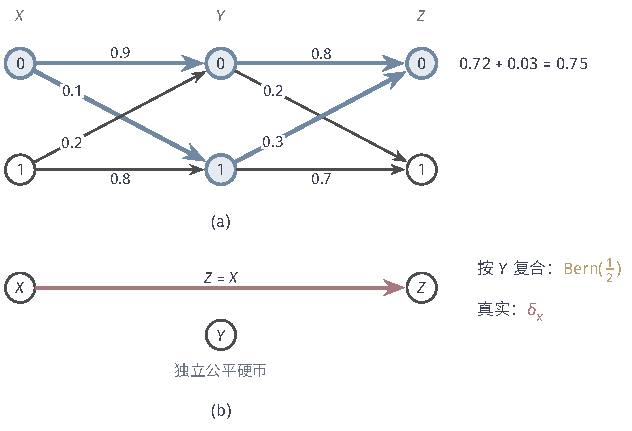
\includegraphics[width=107mm]{figures/07-probability/02-measure-theoretic-probability/tikz/cdis-composition/figure.pdf}
  \caption{核的复合。(a)$X\to Y\to Z$两级转移，边上是转移概率；从$X=0$到$Z=0$的两条路径（蓝）贡献$0.72$与$0.03$，合计$0.75$。(b)$Z=X$、$Y$为独立硬币时，按中间值$Y$复合得到$\operatorname{Bern}(\tfrac12)$（黄），而真实的条件分布是$\delta_x$（红）。}
  \label{fig:cdis-composition}
\end{BookInlineFigure}

\paragraph{条件独立不成立时}
复合公式不能直接用于任意三个随机变量。设$X,Y$是两枚独立的公平硬币，$Z=X$。给定$X$时$Y$仍是公平硬币；$Z=X$与$Y$独立，给定$Y$时$Z$也是公平硬币。按式~\eqref{eq:cdis-composition}复合，得到给定$X=x$时$Z\sim\operatorname{Bern}(\tfrac12)$；可是$Z=X$，真实的条件分布是$\delta_x$。错误在于$Z$与$X$的依赖并不经过$Y$：给定$Y$以后，$X$仍然完全决定$Z$，条件独立不成立。

复合公式对应的是一个两步构造：先有$X$，由$X$产生$Y$，再只由$Y$产生$Z$，依赖只通过中间变量传递。模型若按这种方式给出，条件独立由构造本身保证，复合可以放心使用；对已经给定的三个随机变量，必须先核对$X\perp\!\!\!\perp Z\mid Y$。


\section{本章小结}
\label{sec:cdis-summary}

本章开头问：没有概率表、没有密度，或者条件事件的概率为零时，“给定$Y=y$时$X$的分布”是什么。逐事件的条件概率，即指示函数的条件期望，总是存在，它是只依赖观测信息的随机变量，并且几乎必然满足概率的各条规则；但每条规则的例外集依赖所取的事件，不可数多个事件的版本随意挑选，可能在每个观测值处都拼不成分布。

概率核把这件事组织起来：固定观测值，它是一个概率测度；固定事件，它是观测值的可测函数。概率表中它就是行和为一的矩阵。正则条件分布是与联合规律相容的概率核，判别方法是按观测的分布把核积分回去，必须恢复每个矩形事件的联合概率。条件质量函数、条件密度以及$X=Y$时的单点分布$\delta_y$都通过这一判别。

存在性与唯一性都靠把要求压缩到可数个事件上。目标取实数值时，有理阈值上的分布函数值可数，例外集只并可数次，再用下确界补成分布函数；目标取值于标准Borel空间时，用Borel同构搬到实轴上。观测的取值空间不需要任何结构。两个正则条件分布在一个$P_Y$零测集之外相同，但联合规律不决定核在某个零概率观测值上的值。连续性等附加要求可以在零概率点上选出一个值，但满足要求的版本未必存在，选出的值还依赖用哪个观测量逼近，Borel--Kolmogorov悖论中带子与楔形给出$1$与$2x$两种答案。

表~\ref{tab:cdis-summary}对照了条件期望与条件分布。前者对任意可积随机变量存在，回答“给定信息后平均是多少”；后者要求目标空间有标准Borel结构，回答“给定信息后完整的规律是什么”，并通过积分给出前者的一个版本。

\begin{BookInlineTable}
  \centering
  \caption{条件期望与正则条件分布的对照}
  \label{tab:cdis-summary}
  \begin{tabular}{lll}
    \toprule
    & 条件期望$\mathbb{E}[g(X)\mid Y]$ & 正则条件分布$K(y,\cdot)$ \\
    \midrule
    对象 & 一个随机变量 & 每个$y$一个概率测度 \\
    定义 & 已知事件上积分相等 & 每个事件上取条件概率 \\
    存在 & $g(X)$可积即可 & 目标为标准Borel空间 \\
    唯一 & 几乎必然 & 在$P_Y$零测集之外 \\
    关系 & \multicolumn{2}{c}{$\mathbb{E}[g(X)\mid Y]=\int g(x)\,K(Y,\mathrm{d}x)$，$\mathbb{E}\lvert g(X)\rvert<\infty$} \\
    \bottomrule
  \end{tabular}
\end{BookInlineTable}

对核积分有两种方向。固定观测值、对目标积分，得到条件期望的积分表示，证明沿指示函数、简单函数、单调极限与正负分部进行；条件矩与条件方差就是条件分布的矩与方差。整体矩有限只保证条件矩几乎处处有限；反过来，每个观测值上条件矩有限也推不出整体矩有限。再按观测的分布积分，边缘与核唯一地确定联合规律，计算$f(X,Y)$的期望时可以把观测值代入、只对目标积分。对全部观测值积分得到全概率公式，从另一面看就是混合分布：随机硬币的正面次数是二项分布的均匀混合，t分布是高斯分布的尺度混合。

有限个标准Borel随机对象的联合规律总可以链式分解，每一步的核依赖此前的全部变量；反过来，起始分布和这样一列核唯一地确定一个联合规律，对应逐步的随机构造。在链式分解中省去条件变量，需要条件独立作为依据。

条件独立要求给定信息后对所有有界函数的乘积期望分解，等价于条件联合分布是条件边缘的乘积，也等价于已知条件后再知道$X$不改变$Z$的条件分布；条件协方差为零不够。独立与条件独立互不蕴含，增减条件信息都可能改变独立关系；条件化由联合规律决定，干预的效果还依赖产生数据的机制。给定中间变量条件独立时，核可以复合，有限状态下就是转移矩阵相乘；没有条件独立时复合会给出错误的答案。

这些工具在后面多处使用。给定观测后对未知量的分布作修正，是卷八统计推断的出发点，可参考\BookChapterRef{chap:parametric-statistical-inference}{卷八第1章“参数化统计推断”}。把链式分解与核复合沿时间无限地进行下去，就是随机过程中的转移结构，可参考\BookChapterRef{chap:discrete-time-stochastic-processes}{卷九第3章“离散时间随机过程”}。本卷在第~\ref{chap:sample-generation}章按核逐步产生样本，在第~\ref{chap:information-measures}章用条件分布定义条件熵与互信息。


